\clearpage
\section{Real leptons efficiencies}
\label{App:RealEfficiency}
        This appendix presents more details on the measurement of the real lepton efficiency in data selecting either $Z$ or $t\overline{t}$ events. A general description is given in Section~\ref{App:RealEff_Intro}. The methods and the obtained results are presented in Section \ref{App:RealEff_Z_TandP} ($Z$-measurement) and \ref{App:RealEff_ttbar_TandP} ($t\overline{t}$-measurement). As shown in Section~\ref{sec:RealRate_DD}, the efficiency measured in a sample enriched in $Z$ events is used as input to the matrix method; more details on the evaluation of the associated systematic uncertainties are presented in Section \ref{App:RealEff_Z_Syst}.


%%%%%%%%%%%%%%%%%%
% SUBSECTION 1 
%%%%%%%%%%%%%%%%%%
	\subsection{Description of the real lepton efficiencies}
	\label{App:RealEff_Intro}
	
	The real lepton efficiency is defined as the ratio between the number of (prompt) leptons passing the signal lepton definition and the number of (prompt) leptons passing the baseline definition. Thus, it measures the efficiency of the signal lepton definition cuts with respect to the baseline ones. Table~\ref{tab:lepton_def_appR} shows these definitions. The efficiency associated to each signal cut (given the baseline definition) is shown in Figure \ref{fig:CutEff_MC}, considering either $Z\rightarrow \ell\ell$ (top) or $t\overline{t}$ (bottom) simulated events.  
	
	
%% Definition of the baseline and signal leptons	
%%%%%%%%%%%%%%%%%%%%%%%%%%%%%%%%%%%%%%%%%%%%%%%%%%%%%%%%%%%%%
\begin{table}[htb!] 
	\begin{center}
	    \begin{tabular}{|l|c|c|}
	     \hline
	     \hline
	       & \textbf{Baseline electron} & \textbf{Baseline muon} \\
	     \hline
	     \hline
	     Acceptance     & $\pt > 10\,\mathrm{GeV}\, |\eta^\mathrm{clust}| < 2.47$  & $\pt > 10\,\mathrm{GeV}, |\eta| < 2.5$ \\
	                     &  except $1.37<|\eta^\mathrm{clust}|<1.52$       & \\
	     \hline
	     Quality & {\tt LooseLLH} & {\tt{xAOD::Muon::Medium}} \\
%      \hline
%      Impact parameter &  $|d_0/\sigma(d_0)|<$ 5.0 & - \\
         \hline
         $\ell$-jet Isolation      & $\Delta{}R(e,jet)$~$>$~0.4 & $\Delta{}R(\mu,jet)$~$>$~0.4 \\
         \hline
         Impact parameter & $|d_0/\sigma(d_0)|<5.0$  & \\
         \hline\hline
         & \textbf{Signal Electron} & \textbf{Signal Muon} \\
         \hline
         \hline
         Quality & {\tt TightLLH} & -\\
         & $|\eta|<2.0$  & -\\
         \hline
         Isolation                & $E_{\mathrm{T}}^{\mathrm{topocone20}} / \pt < 0.06$ & $\pt^{\mathrm{varcone30}} / \pt < 0.06$ \\
                                  & $\pt^{\mathrm{varcone20}} / \pt < 0.06$  & \\
         \hline
         Impact parameter & $|z_0 \cdot sin(\mathrm{\theta})|<$ 0.4 mm   & $|z_0 \cdot sin(\mathrm{\theta})|<$ 0.4 mm \\ 
                       &                                     & $|d_0/\sigma(d_0)| < 3.0$\\
         \hline
		\end{tabular}
	\end{center}
\caption{Summary of the electron and muon selection criteria. The signal
  selection requirements are applied on top of the baseline selection. The
  lepton-jet isolation requirement is applied after electron-jet overlap
  removal.}
\label{tab:lepton_def_appR}
\end{table}
%%%%%%%%%%%%%%%%%%%%%%%%%%%%%%%%%%%%%%%%%%%%%%%%%%%%%%%%%%%%	
	
	
%% Efficiencies of the differents cuts as a function of pT
%%%%%%%%%%%%%%%%%%%%%%%%%%%%%%%%%%%%%%%%%%%%%%%%%%%%%%%%%%%%	
\begin{figure}[!htb]
  \begin{center} 
	   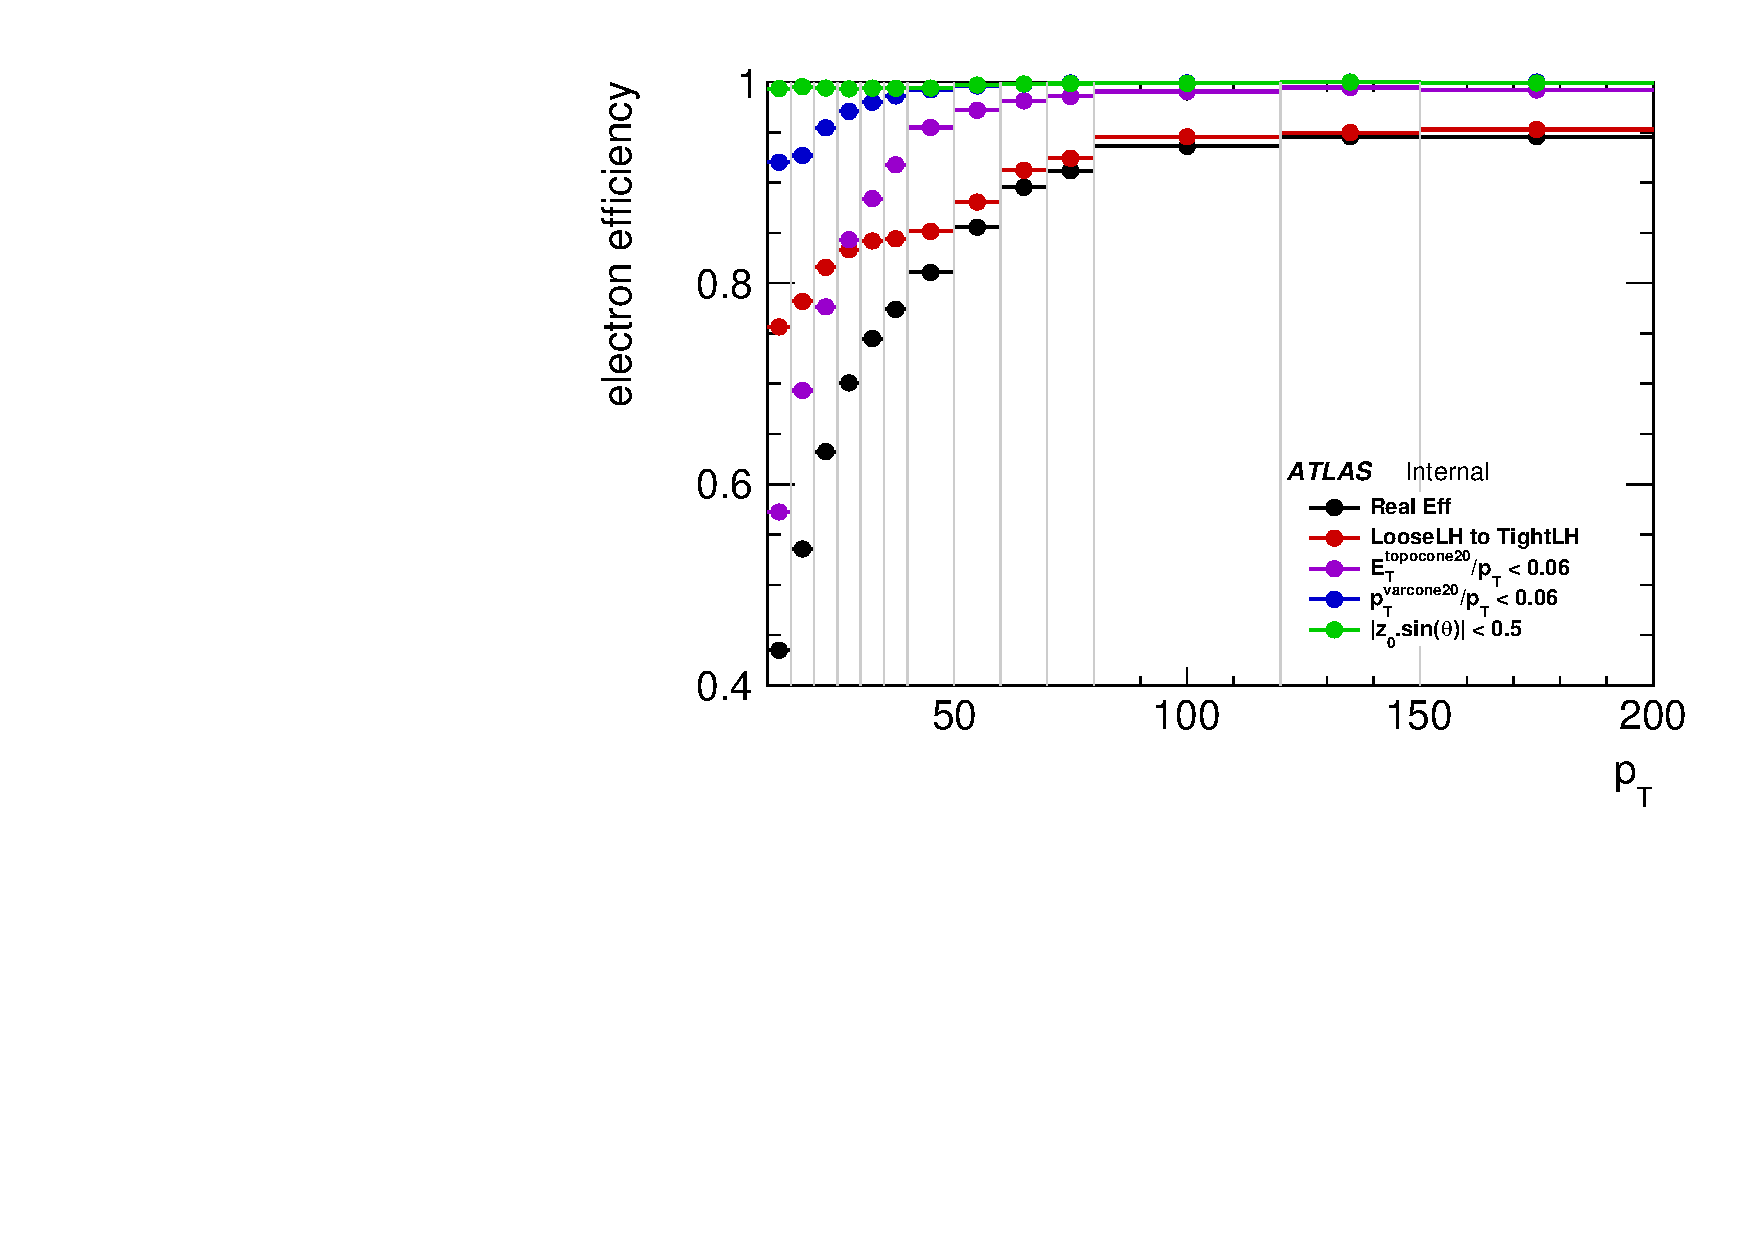
\includegraphics[width=0.45\textwidth]{BKG/realEff/CutEff/TruthMatch_Zee_electrons_CutEff_Vs_pt.pdf} 
	   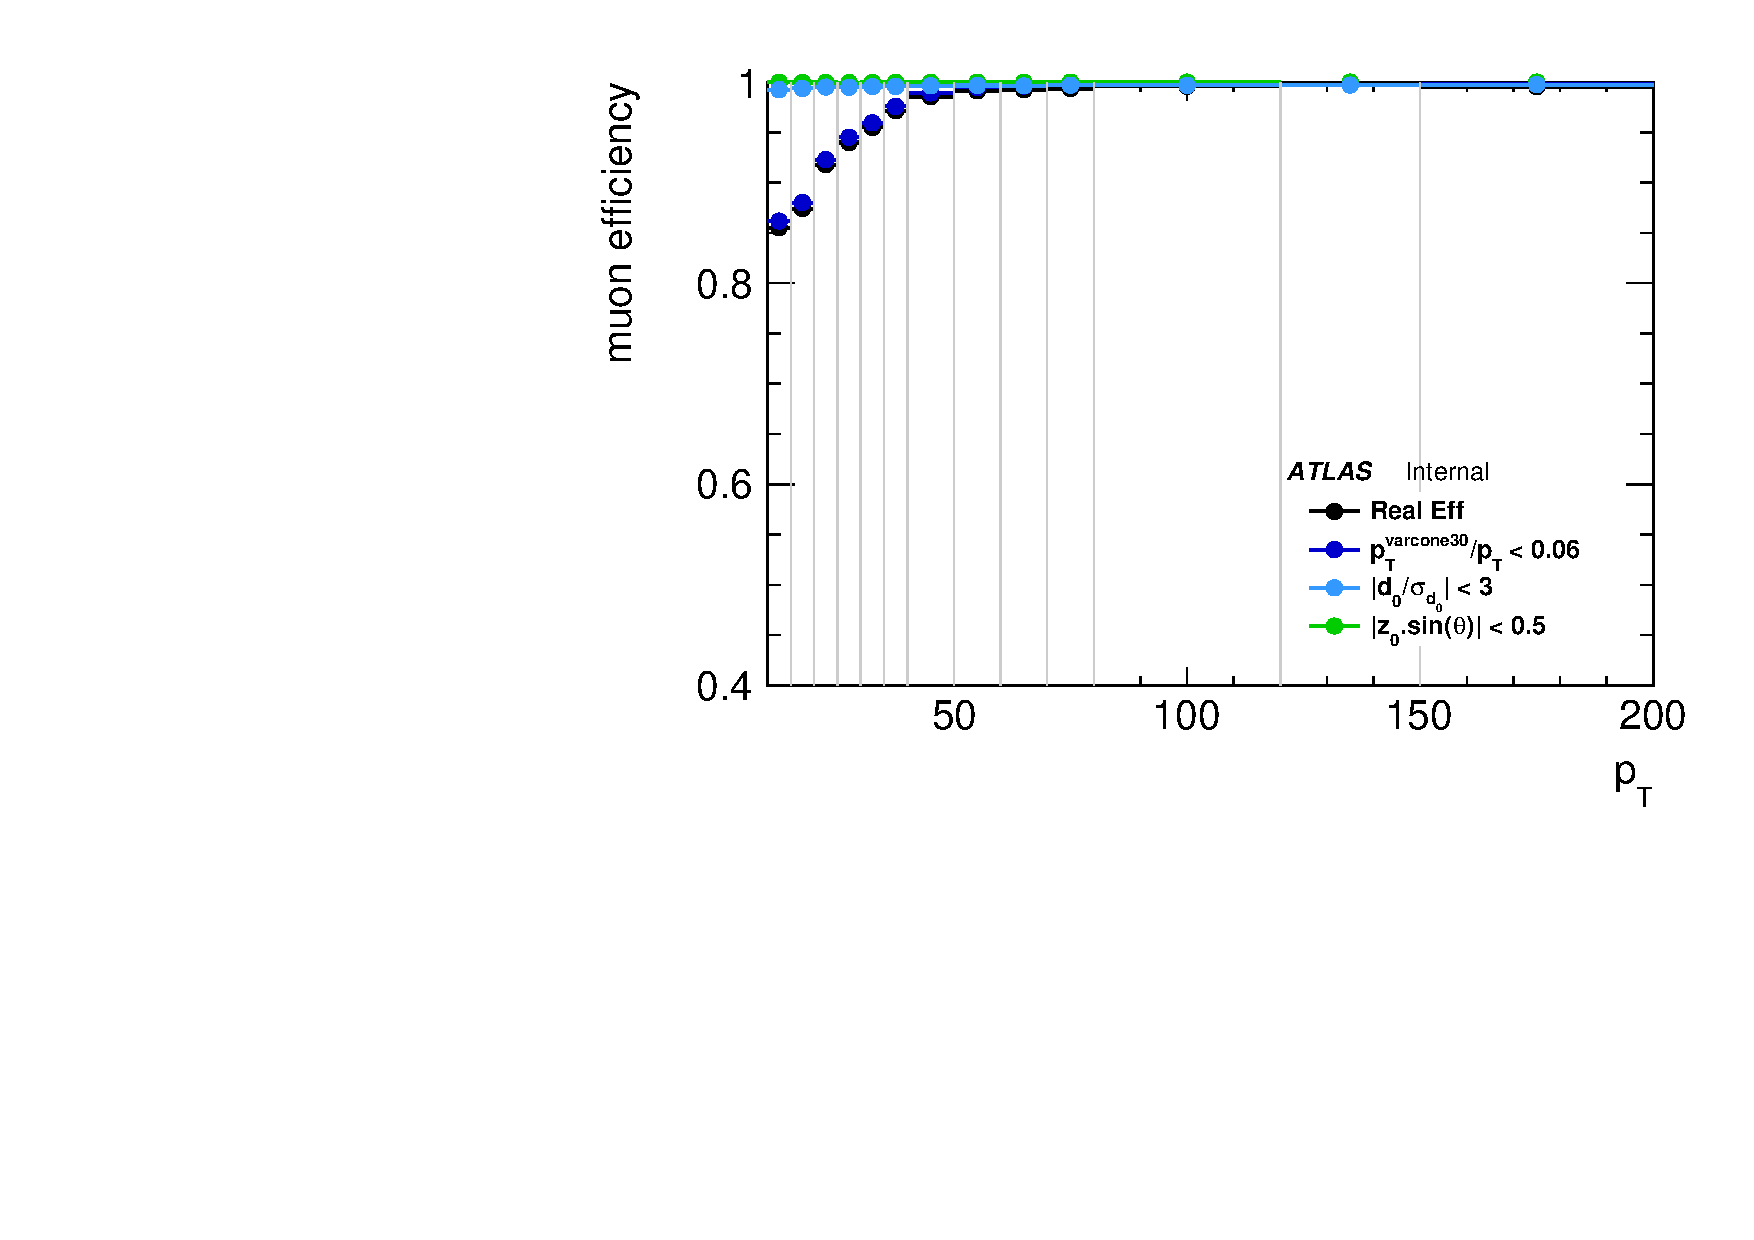
\includegraphics[width=0.45\textwidth]{BKG/realEff/CutEff/TruthMatch_Zmumu_muons_CutEff_Vs_pt.pdf} 
	   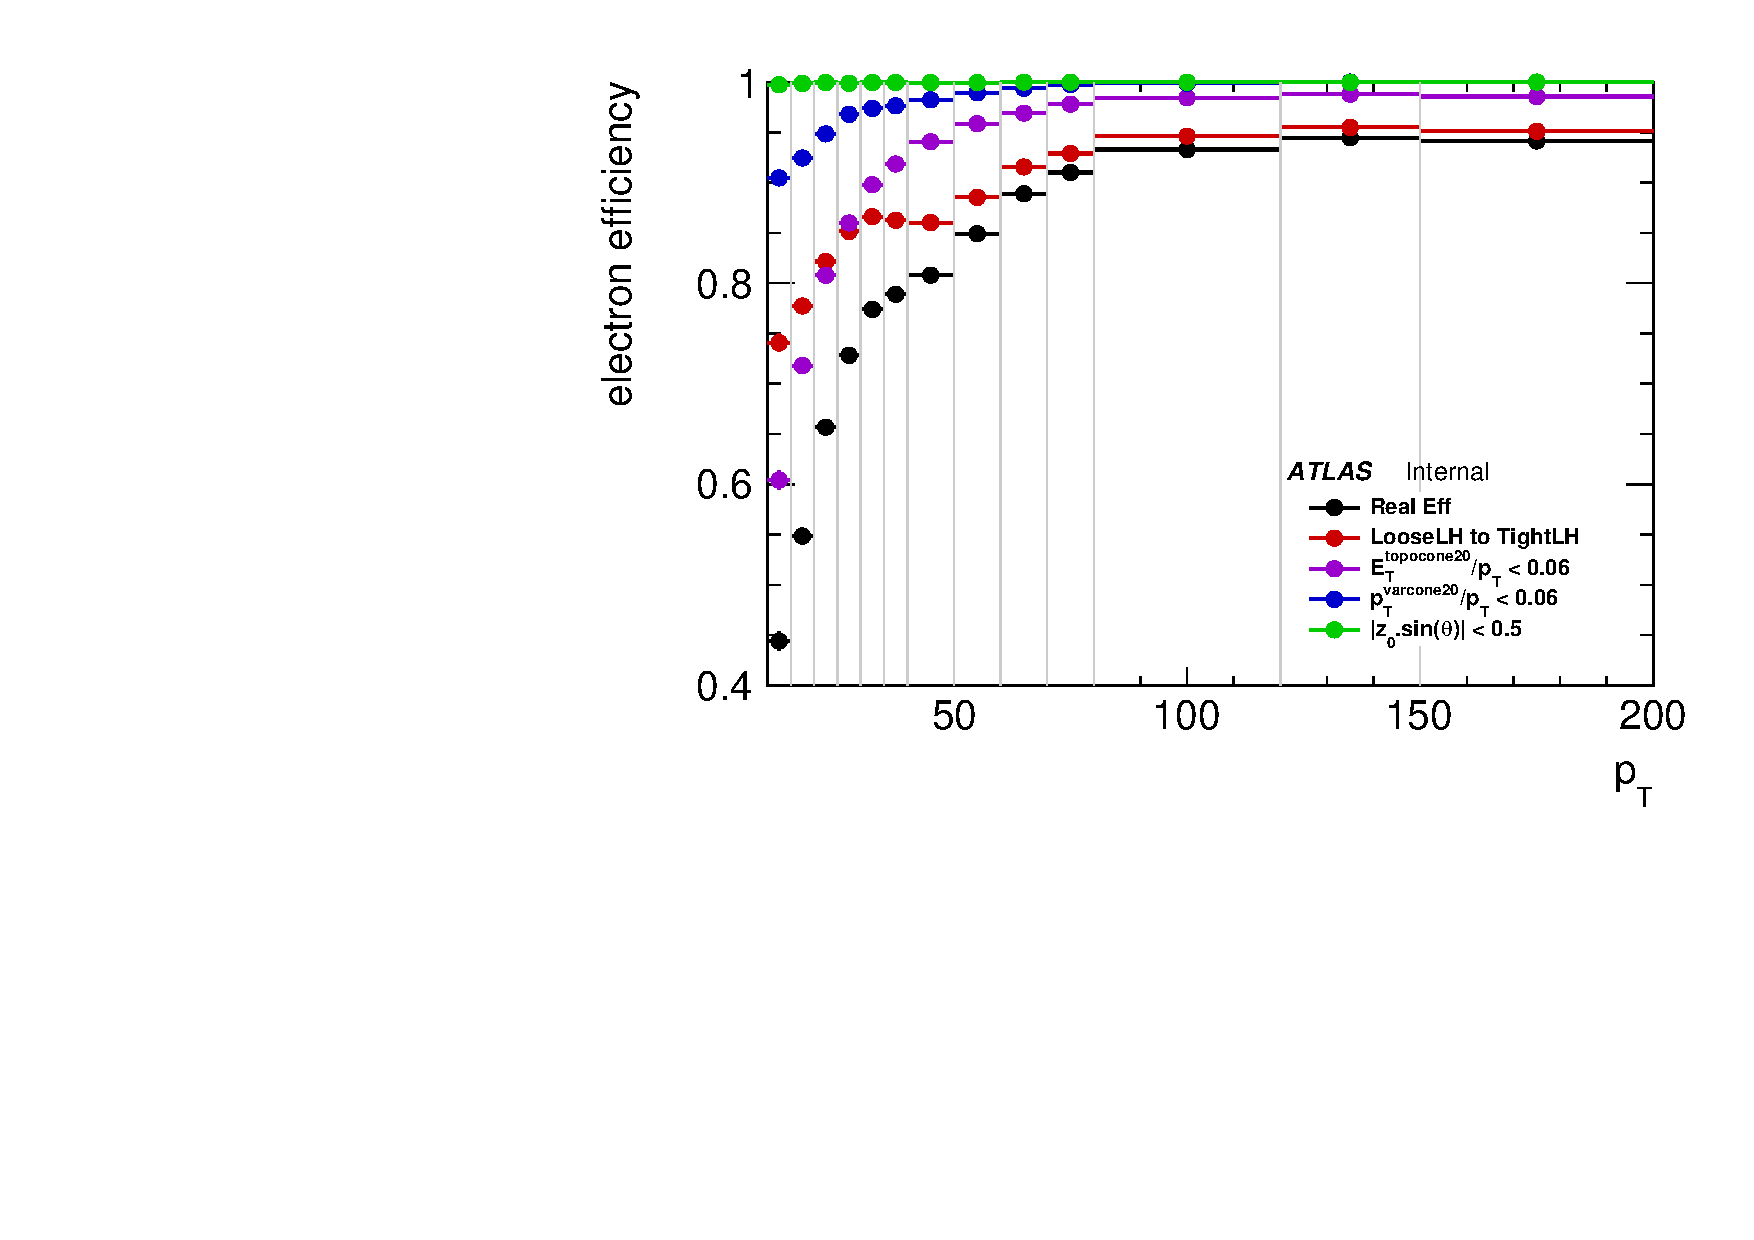
\includegraphics[width=0.45\textwidth]{BKG/realEff/CutEff/TruthMatch_ttbar_electrons_CutEff_Vs_pt.pdf} 
	   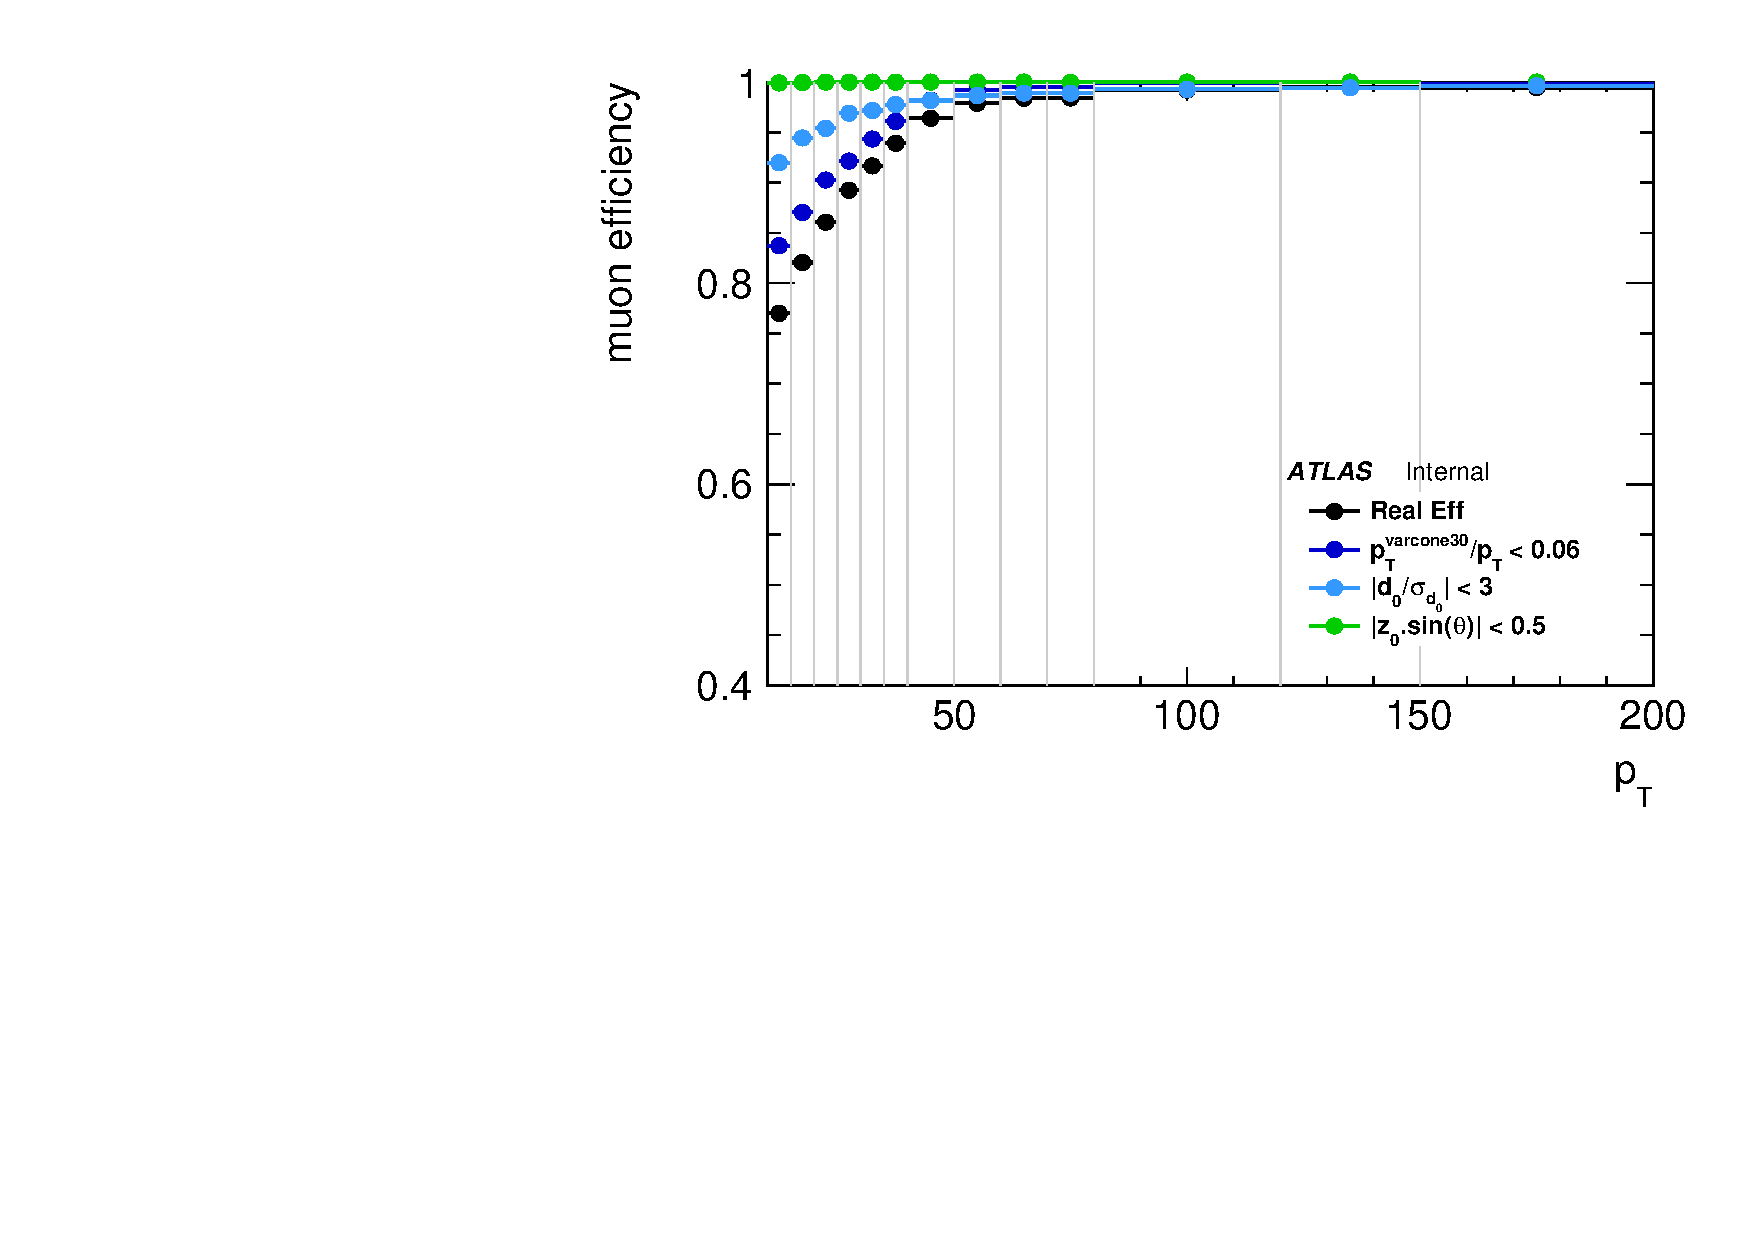
\includegraphics[width=0.45\textwidth]{BKG/realEff/CutEff/TruthMatch_ttbar_muons_CutEff_Vs_pt.pdf} 
	   \caption{\label{fig:CutEff_MC} Efficiencies of the signal electrons (left) and muons (right) definition cuts as a function of $\pt$. The leptons are selected from $Z+jets$ (top) and $t\overline{t}$ (bottom) simulated events using a loose truth match. The black points correspond to the total real lepton efficiency, the purple (dark blue) to the calorimeter (track) isolation criteria, the light blue (green) to the cut on transverse (longitudinal) impact parameter and the red points to the tight likelihood electron identification efficiency with respect to the loose likelihood electron identification.}
  \end{center}
\end{figure}				
%%%%%%%%%%%%%%%%%%%%%%%%%%%%%%%%%%%%%%%%%%%%%%%%%%%%%%%%%%%%	

	
	\par{\bf Discussion on real electron efficiency \\}
        The left plots from Figure \ref{fig:CutEff_MC} shows that the prompt electron efficiency increase from $\sim 45\%$ in the [10-25] GeV \pt range to $\sim 95\%$ when $\pt > 80$ GeV. The dominant contribution to the electron efficiency losses is the tight likelihood (LH) identification cut in the $\pt > 25$ GeV range and the calorimeter isolation requirement in the  $\pt < 25$ GeV range. The loose LH to tight LH efficiency increase form $\sim 75\%$ to $\sim 84\%$ in the [10-25] GeV \pt range to reach a plateau at $\sim 84\%$ in the [25-50] range and increase again to reach a $\sim 95\%$ efficiency plateau at 80 GeV. The calorimeter isolation cut efficiency increase form $\sim 58\%$ at low \pt to a $\sim 99\%$ plateau at $\pt > 80$ GeV for the $Z+jets$ ($t\overline{t}$) processes. The efficiency associated to the track isolation cut is $\sim 93\%$ in the [10-15] GeV \pt range and the increase up to a $\sim 100\%$ efficiency plateau at $\pt > 60$ GeV. The contribution of the longitudinal impact parameter cut to the real efficiency is negligible. Only few percent efficiencies differences are observed between $Z\rightarrow ee$ and $t\overline{t}$ electron efficiencies mostly driven by the calorimeter isolation at high \pt. 

	\par{\bf Discussion on real muon efficiency \\}
        As the same muon identification is used for the baseline and the signal definitions, the muon efficiencies are much higher than the electron ones. The associated efficiencies computed using $Z\rightarrow\mu\mu$ events increases from $\sim 85\%$ at low \pt to a $\sim 99\%$ efficiency plateau at $\pt > 60$. The dominant contribution to the muon efficiency is the track isolation cut. The associated efficiency increases from $\sim 85\%$ at low \pt up to a $\sim 99\%$ efficiency plateau at $\pt > 50$ GeV. An other difference with electrons is that a tight longitudinal impact parameter cut is used in the muons signal definition while this cut it is already used at baseline level in the electron case. The impact of this cut on muon efficiency is negligible for $Z\rightarrow\mu\mu$ events but is sizeable in $t\overline{t}$ as $b$-jets are present in the final state. The associated efficiencies for $t\overline{t}$ processes vary from $\sim 93\%$ at low \pt to $\sim 99\%$ at $\pt > 80$ GeV and become the dominant cut $\pt >$ 50 GeV. As a result, the $t\overline{t}$ efficiencies are lower than the $Z\rightarrow\mu\mu$ ones by $\sim 5\%$ at low \pt and $\sim 1\%$ for $\pt > 80$ GeV.


	
%%%%%%%%%%%%%%%%%%
% SUBSECTION 2 
%%%%%%%%%%%%%%%%%%
	\subsection{Real leptons efficiency measured using $Z$ events}  
	\label{App:RealEff_Z_TandP}
\par{\bf Presentation of the method \\}
         The leptons used for the efficiencies measurements are extracted from data using $Z\rightarrow ee/\mu\mu$ events with a tag-and-probe method. The tag lepton is imposed to pass the signal lepton requirement, $\pt > 25$ GeV and to be matched to the relevant primary single lepton trigger. In the case of the $Z\rightarrow ee$ events a additional $|\eta| < 2$ requirement is used for the tag selection. The probe lepton, used for the real efficiencies measurements, should pass the baseline lepton requirements. The invariant mass of the two leptons should satisfy 80 $ < m_{\ell\ell} < $ 100 GeV and the two leptons are requested to have opposite charge and same flavour. For each tag-and-probe lepton pairs, both leptons are alternatively considered as the possible tag to avoid any bias in the choice of the tag and to increase the statistics. Data to Monte Carlo comparison of the tag-and-probe electron pair invariant mass distributions ($m_{ll}$) shown in Figure \ref{fig:Data_Vs_MC_mll_distributions} shows that background subtraction is only needed for electron with $\pt < 20$ GeV. Similar plots dedicated to muons shows that the muon background contamination is marginal over the whole \pt range.\\


%% MC to Data distributions mll comparison
%%%%%%%%%%%%%%%%%%%%%%%%%%%%%%%%%%%%%%%%%%%%%%%%%%%%%%%%%%%%	
     \begin{figure}[!htb]
	  \begin{center} 
	   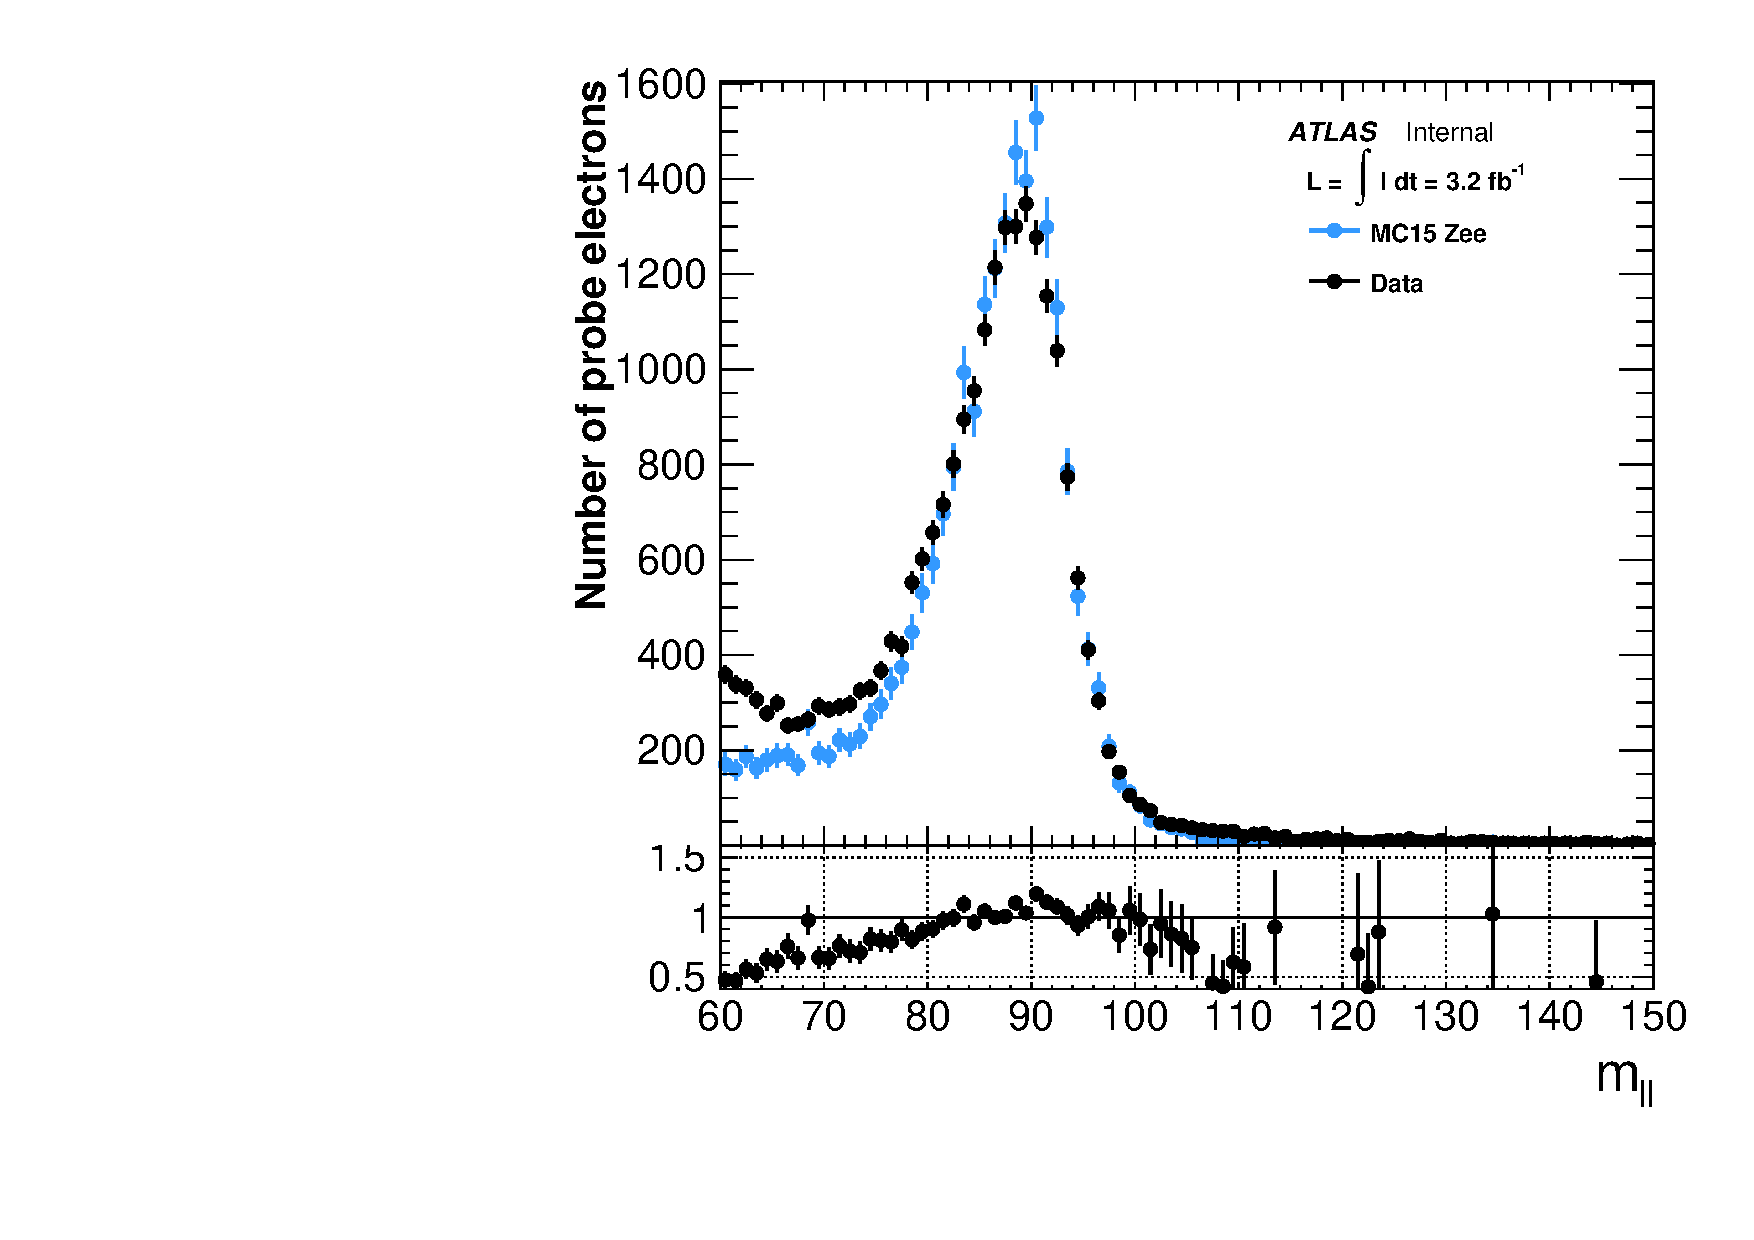
\includegraphics[width=0.4\textwidth]{BKG/realEff/Background_subtraction/DataMergedData_Vs_MC15_electrons_baseline_mll_10_15_ZTandP.pdf}
	   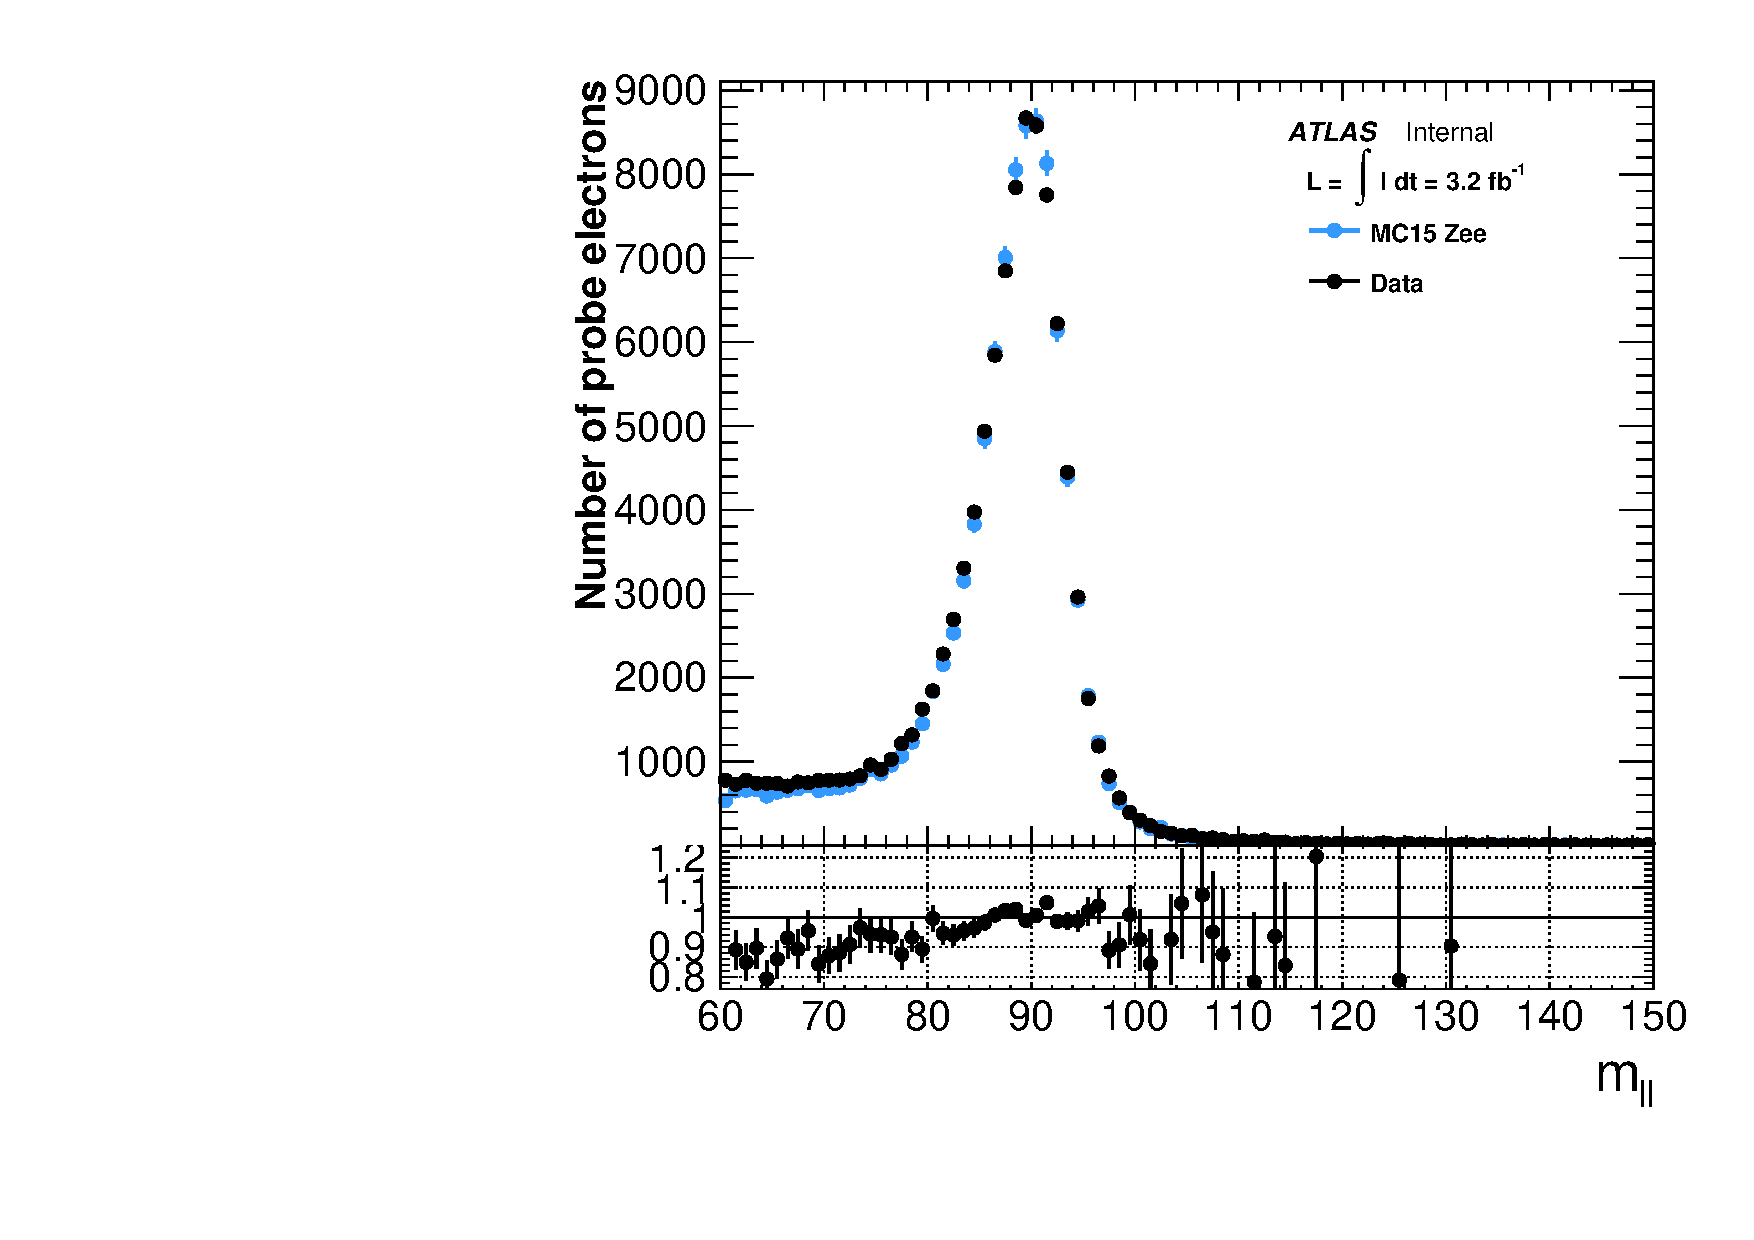
\includegraphics[width=0.4\textwidth]{BKG/realEff/Background_subtraction/DataMergedData_Vs_MC15_electrons_baseline_mll_20_25_ZTandP.pdf} 
	   \caption{\label{fig:Data_Vs_MC_mll_distributions} Distributions of the electron tag-and-probe pairs invariant mass ($m_{\ell\ell}$) computed using $Z$+$jets$ Monte Carlo simulations (light blue) and 2015 run~2 data (black points). The left (right) plot shows the $m_{\ell\ell}$ computed with probe electrons in the [10-15] ([20-25]) GeV \pt range. The Monte Carlo distributions are normalized to the data using a Gaussian fit of the Z mass peak ($85 < m_{\ell\ell} < 95$ GeV).}
	  \end{center}
	\end{figure}	
%%%%%%%%%%%%%%%%%%%%%%%%%%%%%%%%%%%%%%%%%%%%%%%%%%%%%%%%%%%%

The background contamination associated to these low \pt electrons is estimated using a background template method similar to the one used by the $e/\gamma$ performance group for their efficiency measurements~\cite{ATLAS-CONF-2014-018}. The following formula summarize the real lepton efficiencies definition computed with the number of probe electron passing the baseline ($N_{\mathrm{Baseline}}$), signal ($N_{\mathrm{Signal}}$) lepton definitions and the estimated baseline probe lepton background contamination ($N^{\mathrm{Bkg}}_{\mathrm{Baseline}}$)\footnote{As the background contamination is found to be negligible for signal electrons, no background subtraction is done for signal electrons.}.

                                    $$ \epsilon = \frac{ N_{\mathrm{Signal}} }{ N_{\mathrm{Baseline}} - N^{\mathrm{Bkg}}_{\mathrm{Basline}} } $$  
 

\par{\bf Evaluation of the background contamination\\}

        The background contamination has been evaluated on data using a background template method. A sample enriched in background is obtained by reverted loose calorimeter and track isolation cuts and requesting the electron object to fail the medium LH identification. Two variation of the background template definition has been also defined to asses a systematic on the template definition. Table \ref{tab:bkg_templates_def} summarize the background template definitions. The $m_{\ell\ell}^{\mathrm{Temp}}$ distribution associated to the template is then used to estimate the amount of background in the measurement region ($80 < m_{\ell\ell} < 100$ GeV). \\


%% Background template definitions table
%%%%%%%%%%%%%%%%%%%%%%%%%%%%%%%%%%%%%%%%%%%%%%%%%%%%%%%%%%%%
\begin{table}[htb!]
        \begin{center}
        \begin{tabular}{|l|c|c|c|}
        \hline 
        \textbf{cuts \textbackslash{} template} & \textbf{Variation 1} & \textbf{baseline} & \textbf{Variation 2}\tabularnewline
        \hline 
        \hline 
        \textbf{Identification} & - & fail $\texttt{mediumLH}$ & fail $\texttt{mediumLH}$\tabularnewline
        \hline 
        \textbf{Calorimeter Isolation} & $E_{\mathrm{T}}^{\mathrm{topocone20}}/\pt>20\%$  & $E_{\mathrm{T}}^{\mathrm{topocone20}}/\pt>15\%$ & $E_{\mathrm{T}}^{\mathrm{topocone20}}/\pt>20\%$\tabularnewline
        \hline 
        \textbf{Track Isolation} & $\pt^{\mathrm{varcone20}}/\pt>15\%$ & $\pt^{\mathrm{varcone20}}/\pt>8\%$ & $\pt^{\mathrm{varcone20}}/\pt>15\%$\tabularnewline
        \hline 
        \end{tabular}
        \caption{\label{tab:bkg_templates_def} Definitions of the the background templates cuts used to estimate the background contamination associated to the $Z$ tag-and-probe method.} 
        \end{center}
\end{table}
%%%%%%%%%%%%%%%%%%%%%%%%%%%%%%%%%%%%%%%%%%%%%%%%%%%%%%%%%%%%

 As the templates cuts also removes background objects, the templates has to be normalized to provide the correct background estimates. The $120 < m_{\ell\ell} < 150$ GeV region is used for this normalisation as less prompt electrons contribution is expected in the upper $m_{\ell\ell}$ tail. The background in the tail is estimated by integrating the baseline $m_{\ell\ell}$ distributions in this region after subtracting the prompt electron contribution. As the signal electron definitions allows to get a pure sample of prompt lepton, the prompt lepton contamination is estimated by integrating the signal $m_{\ell\ell}^{\mathrm{Sig}}$ distribution divided by the real electron efficiency computed using Monte Carlo simulation. \\
    The baseline electron selection already provides a relatively pure sample of prompt electrons. Therefore the background template suffers from low statistics in the tails. To avoid any bias in the normalisation factor due to statistical fluctuations, the template is fitted using an exponential using the following $m_{\ell\ell}^{\mathrm{Temp}}$ range : $m_{\ell\ell}^{\mathrm{Temp}} [60-80]\cup[100-120]$ GeV. The $80 < m_{\ell\ell} < 100$ range is removed from the fit to get rid of eventual prompt lepton contamination arising from $Z\rightarrow ee$ events. As the low $m_{\ell\ell}$ tail of the templates is statistically dominating, the fit is mostly driven by the $m_{\ell\ell}^{\mathrm{Temp}} [60-80]$ range. The background contamination is then :

$$ N^{\mathrm{Bkg}}_{\mathrm{Baseline}}=\int_{80}^{100}N_{\mathrm{Temp}}~dm_{\ell\ell} \cdot \frac{N_{\mathrm{Baseline}}^{\mathrm{Tail}}-N_{\mathrm{Signal}}^{\mathrm{Tail}}/\epsilon_{Z\rightarrow ee}^{\mathrm{MC}}}{N_{\mathrm{Temp}}^{\mathrm{Tail}}} $$

   The background estimates are summarized in table \ref{tab:efficiency_bkg_estimates}. The estimated background contribution in the [10-15] GeV \pt range is relatively small as it represents less than $1\%$ of the baseline statistics. Low background contamination is also observed in the central region ($|\eta| < 0.8$) with less than $1\%$ of the baseline statistics. This is expected as the electron identification is better in central region of the calorimeter and the hadronic background contribution decreases with \pt.


%% Background estimates table
%%%%%%%%%%%%%%%%%%%%%%%%%%%%%%%%%%%%%%%%%%%%%%%%%%%%%%%%%%%%
\begin{table}[htb!]
        \begin{center}
        \begin{tabular}{|l|c|c|c|} 
        \hline 
        \hline 
        \textbf{$\pt$ \textbackslash{} $|\eta|$} & \textbf{{[}0-0.8{]}} & \textbf{{[}0.8-1.37{]}} & \textbf{{[}1.52-2.0{]}}\tabularnewline
        \hline 
        \hline 
        \textbf{{[}10-15{]} GeV} & $0.9\pm0.7$ & $3.2\pm0.7$ & $4.6\pm0.5$\tabularnewline
        \hline 
        \textbf{{[}15-20{]} GeV} & $0.1\pm0.1$ & $0.7\pm0.2$ & $0.9\pm0.2$\tabularnewline
        \hline 
        \end{tabular}
        \end{center}
        \caption{\label{tab:efficiency_bkg_estimates} Background contamination (in $\%$) estimated using the template method. The \pt and $\eta$ binning corresponds to the ones used for the final measurements.}
\end{table}        
%%%%%%%%%%%%%%%%%%%%%%%%%%%%%%%%%%%%%%%%%%%%%%%%%%%%%%%%%%%%


Figure \ref{fig:bkg_templates_closure} shows the baseline $m_{\ell\ell}$ distributions before and after background template subtraction. The data after background subtraction is compared to Monte Carlo simulations and the template distribution and their corresponding fit are also shown. The simulated $m_{\ell\ell}$ distributions are normalized to the data after background subtraction using a Gaussian fit in the $85 < m_{\ell\ell} < 95$ GeV range. The top and the bottom plots corresponds to the $10 < \pt < 15$ GeV range and the $15 < \pt < 20$ GeV range respectively. The left, middle and right plots correspond to the $|\eta| < 0.8$, $0.8 < |\eta| < 1.37$ and $1.52 < |\eta| < 2.$ ranges respectively. After background subtraction, the data agree well with the Monte Carlo simulation within the statistical uncertainties and a flat data to MC ratio is observed for all the \pt and $|\eta|$ ranges. The largest improvements are observed in the $\pt[10-15] \cup |\eta|[0.8-2.0]$ range where a sizeable background contamination is subtracted.

        

%% Background estimates 'closure test'
%%%%%%%%%%%%%%%%%%%%%%%%%%%%%%%%%%%%%%%%%%%%%%%%%%%%%%%%%%%%	
\begin{figure}[!htb]
  \begin{center} 
	   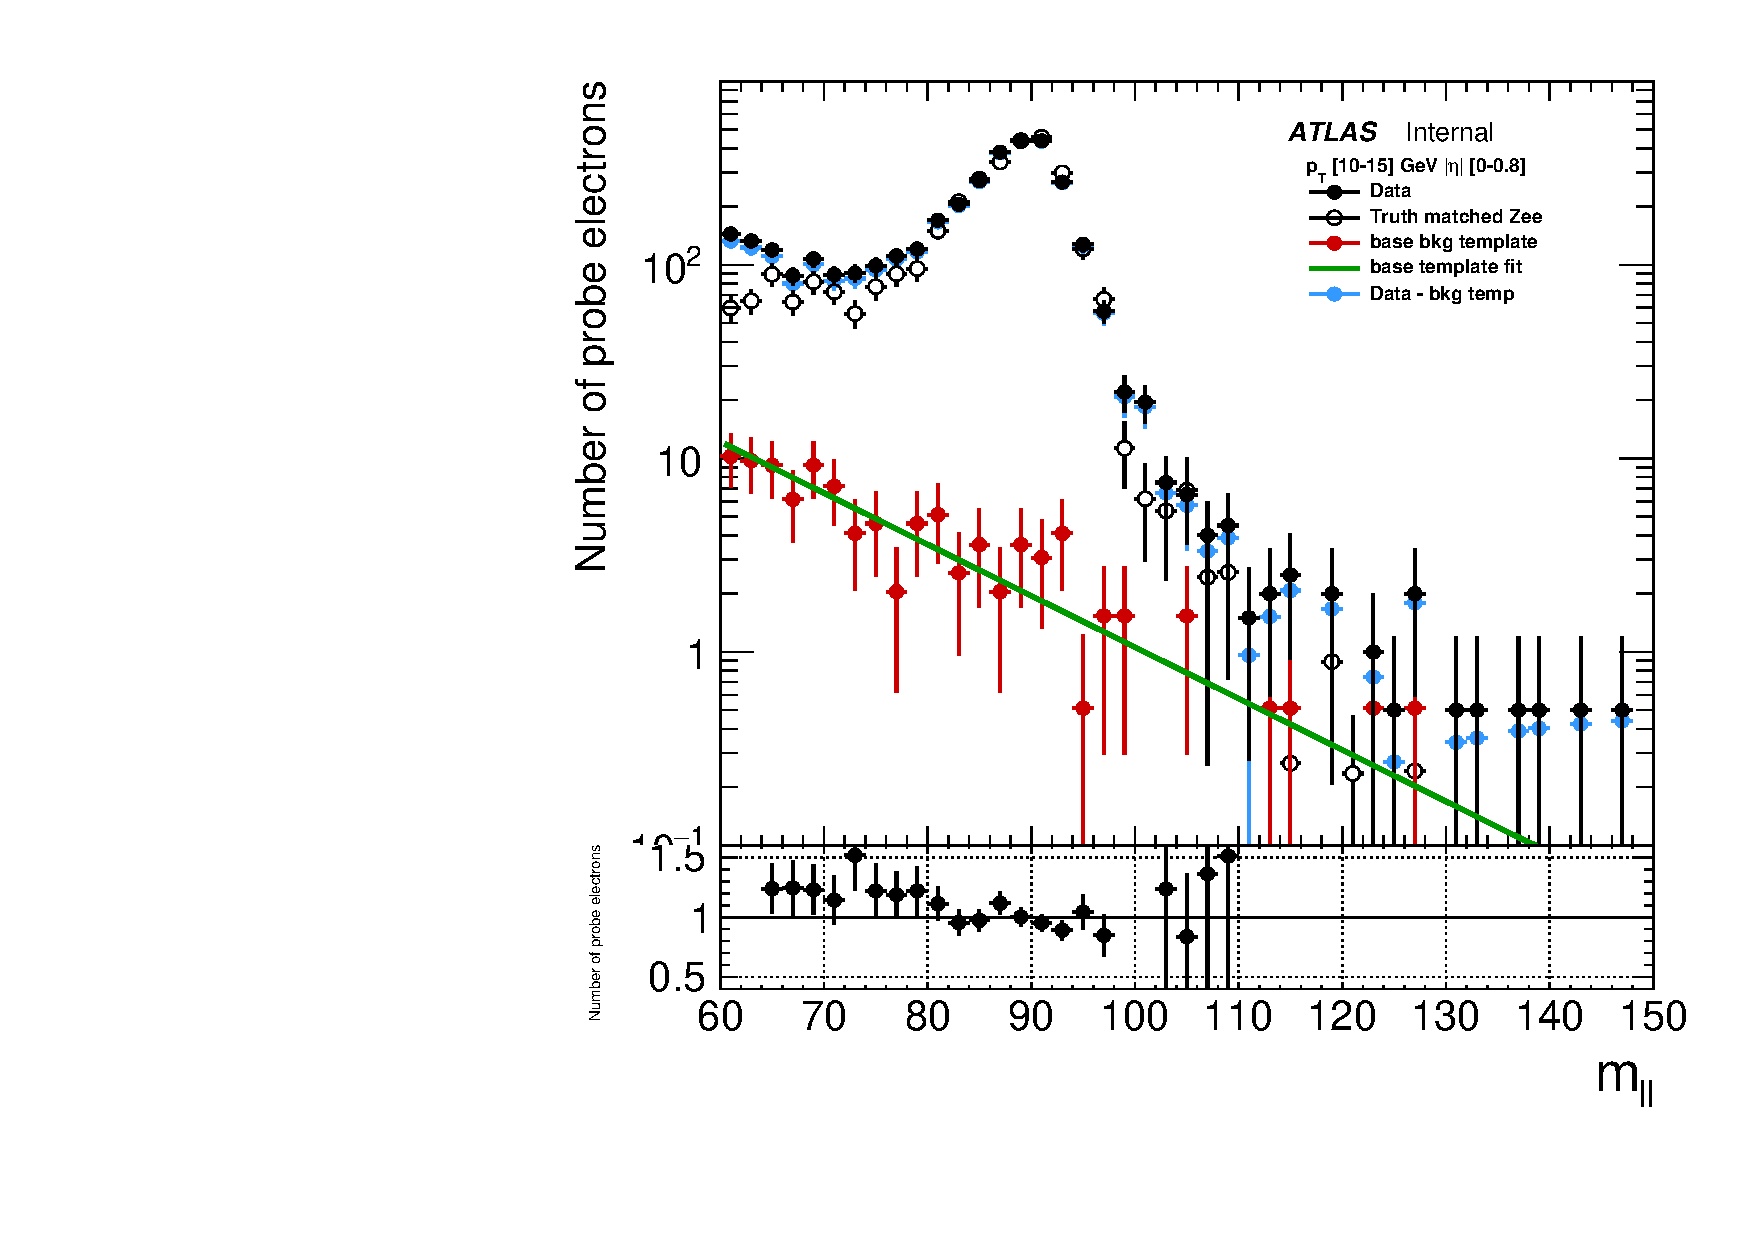
\includegraphics[width=0.30\textwidth]{BKG/realEff/Background_subtraction/Data_background_template_electrons_ZTandP_logScale_10_15_00_08_closure_test.pdf} 
	   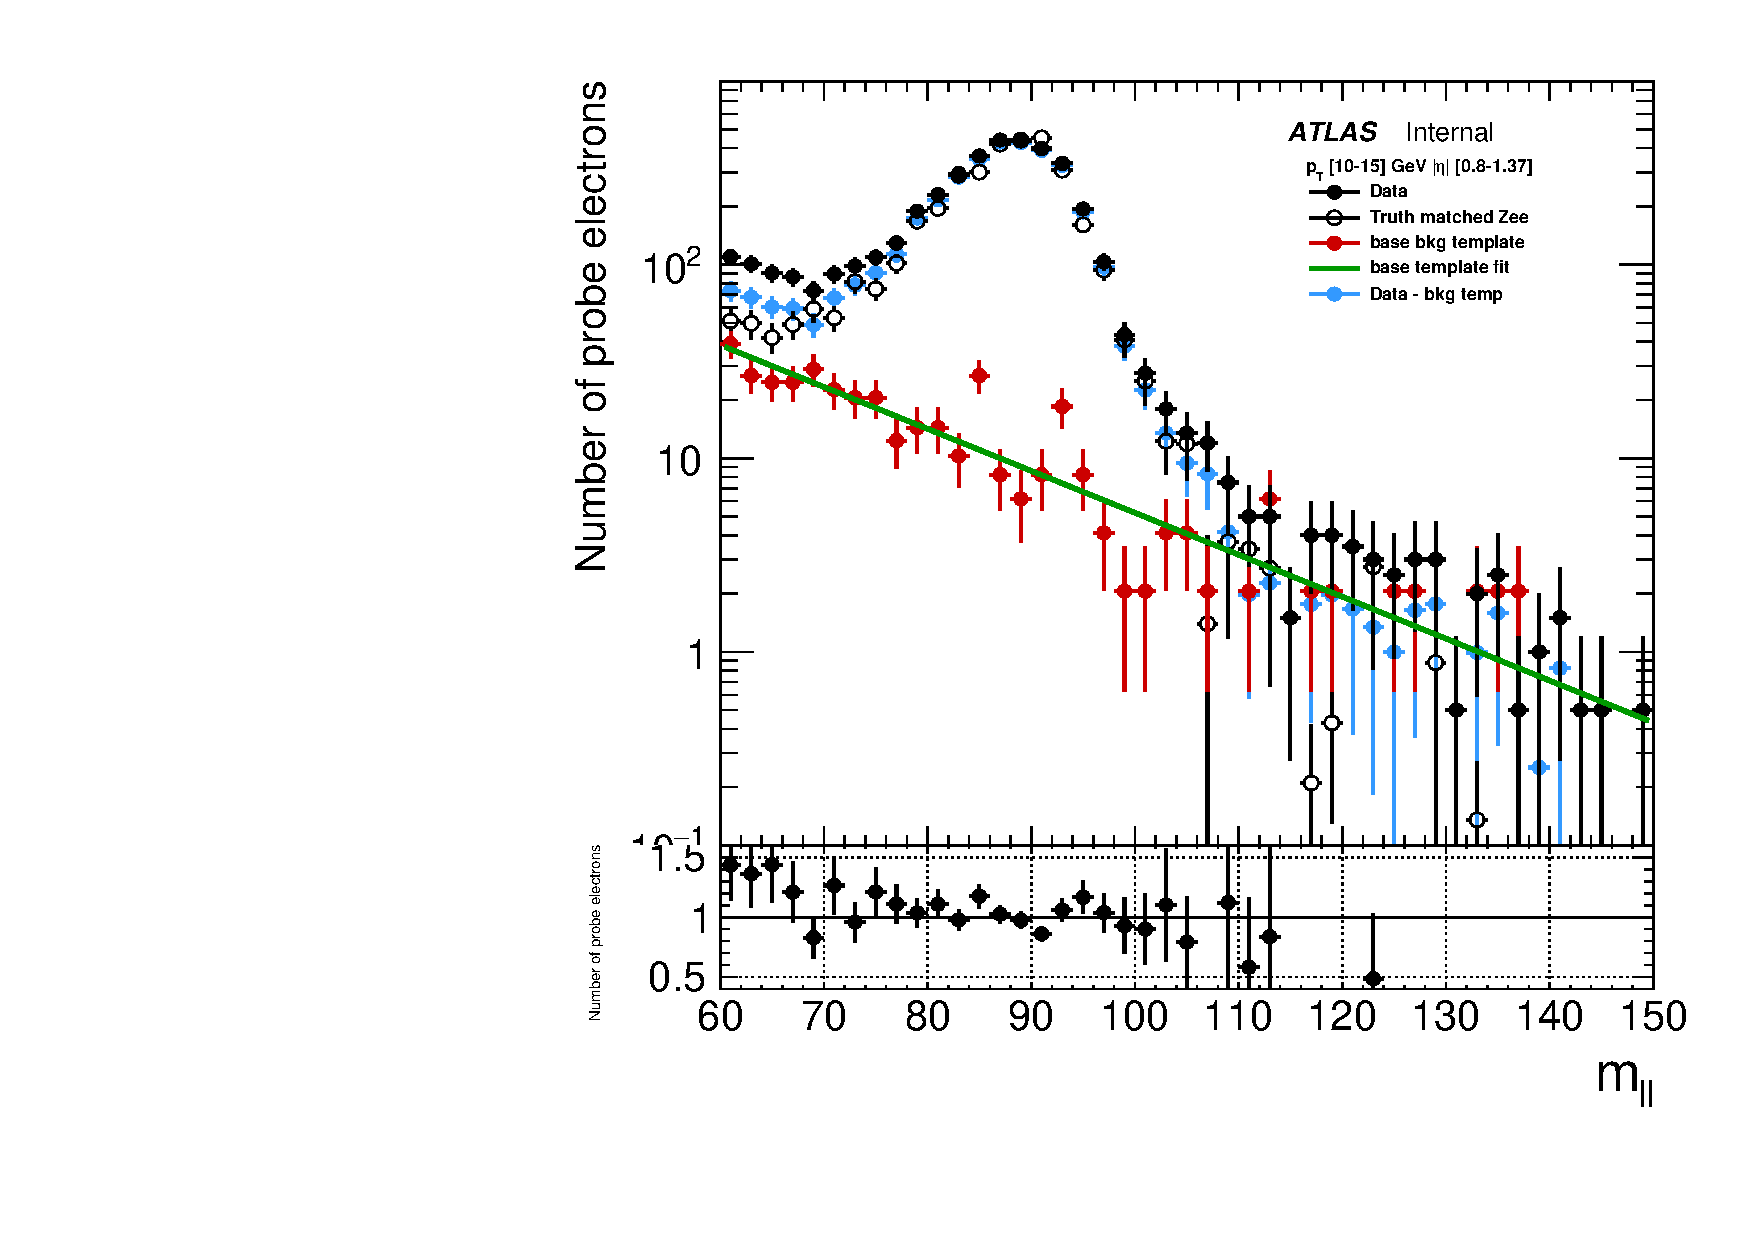
\includegraphics[width=0.30\textwidth]{BKG/realEff/Background_subtraction/Data_background_template_electrons_ZTandP_logScale_10_15_08_137_closure_test.pdf} 
	   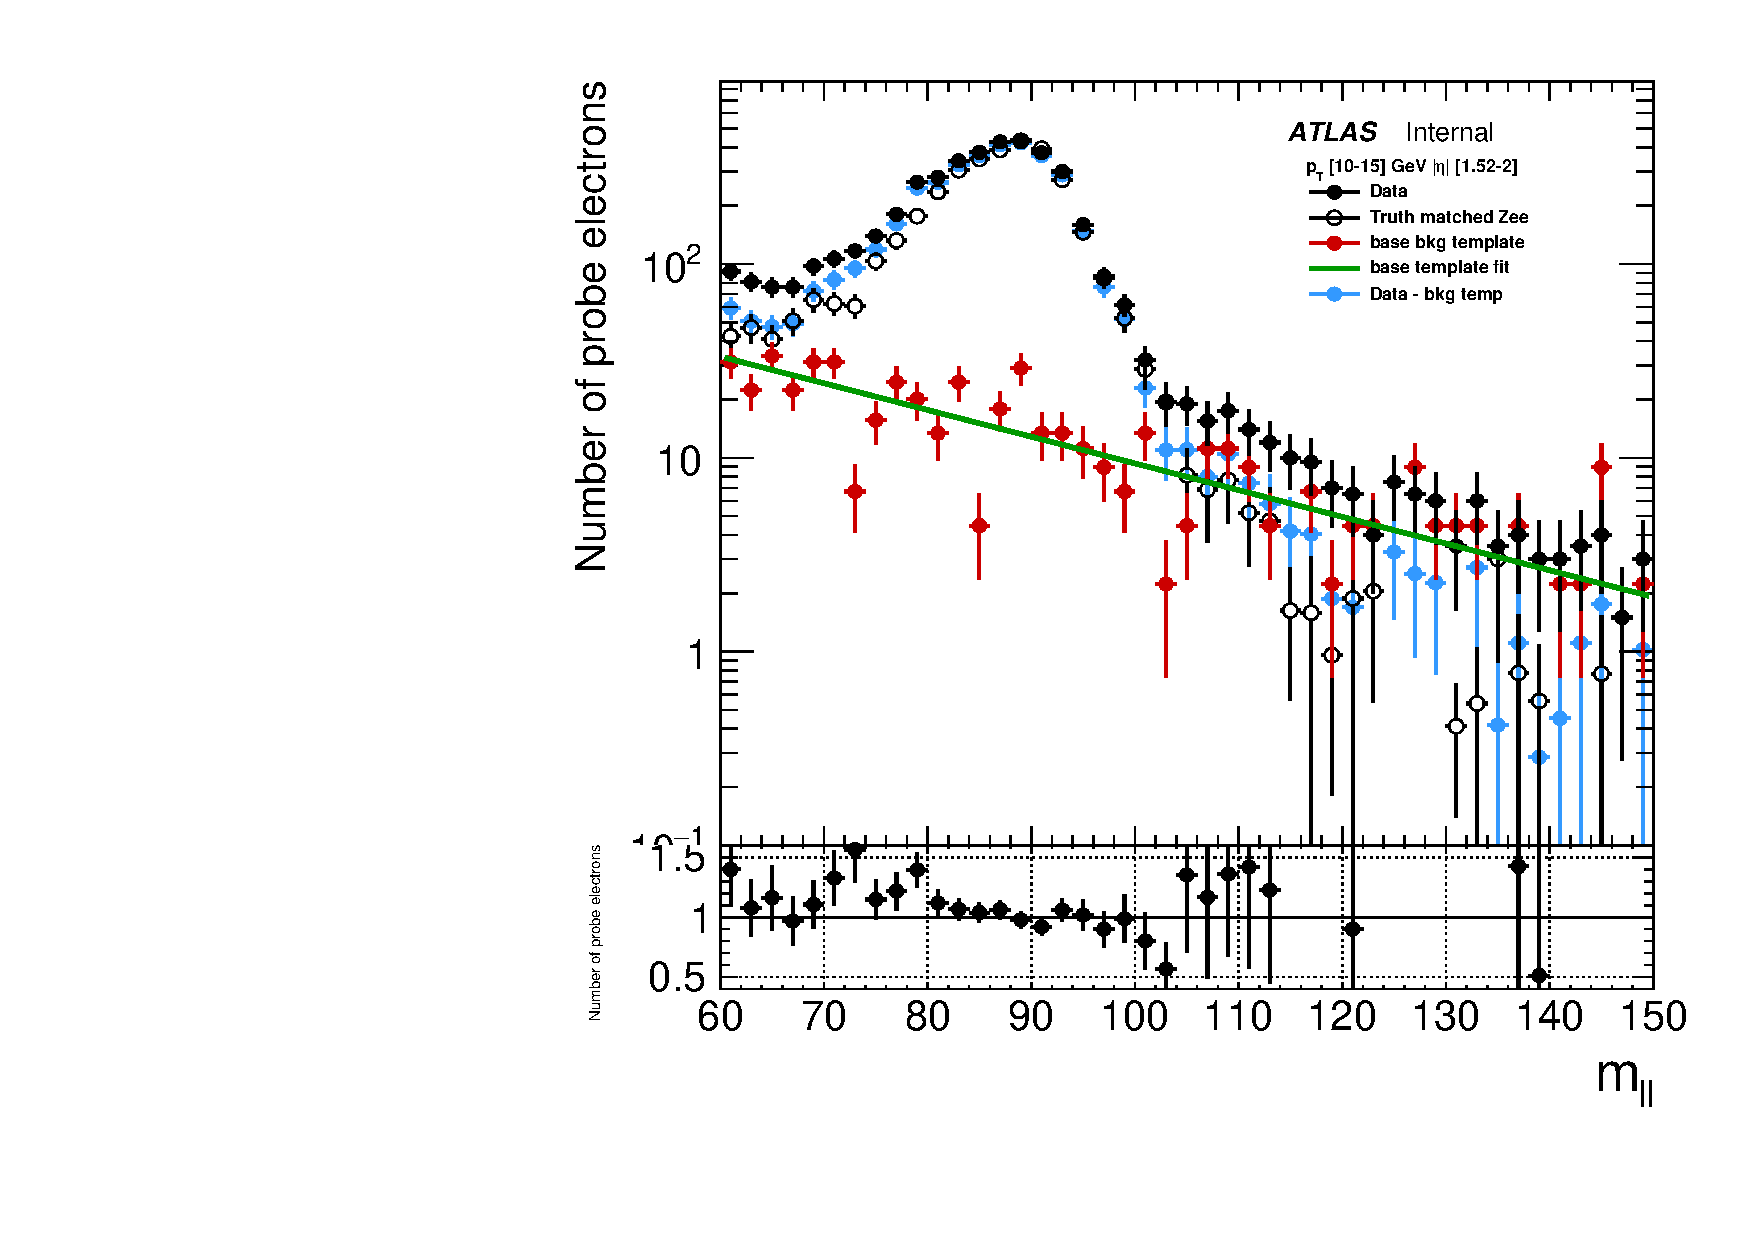
\includegraphics[width=0.30\textwidth]{BKG/realEff/Background_subtraction/Data_background_template_electrons_ZTandP_logScale_10_15_152_20_closure_test.pdf}
	   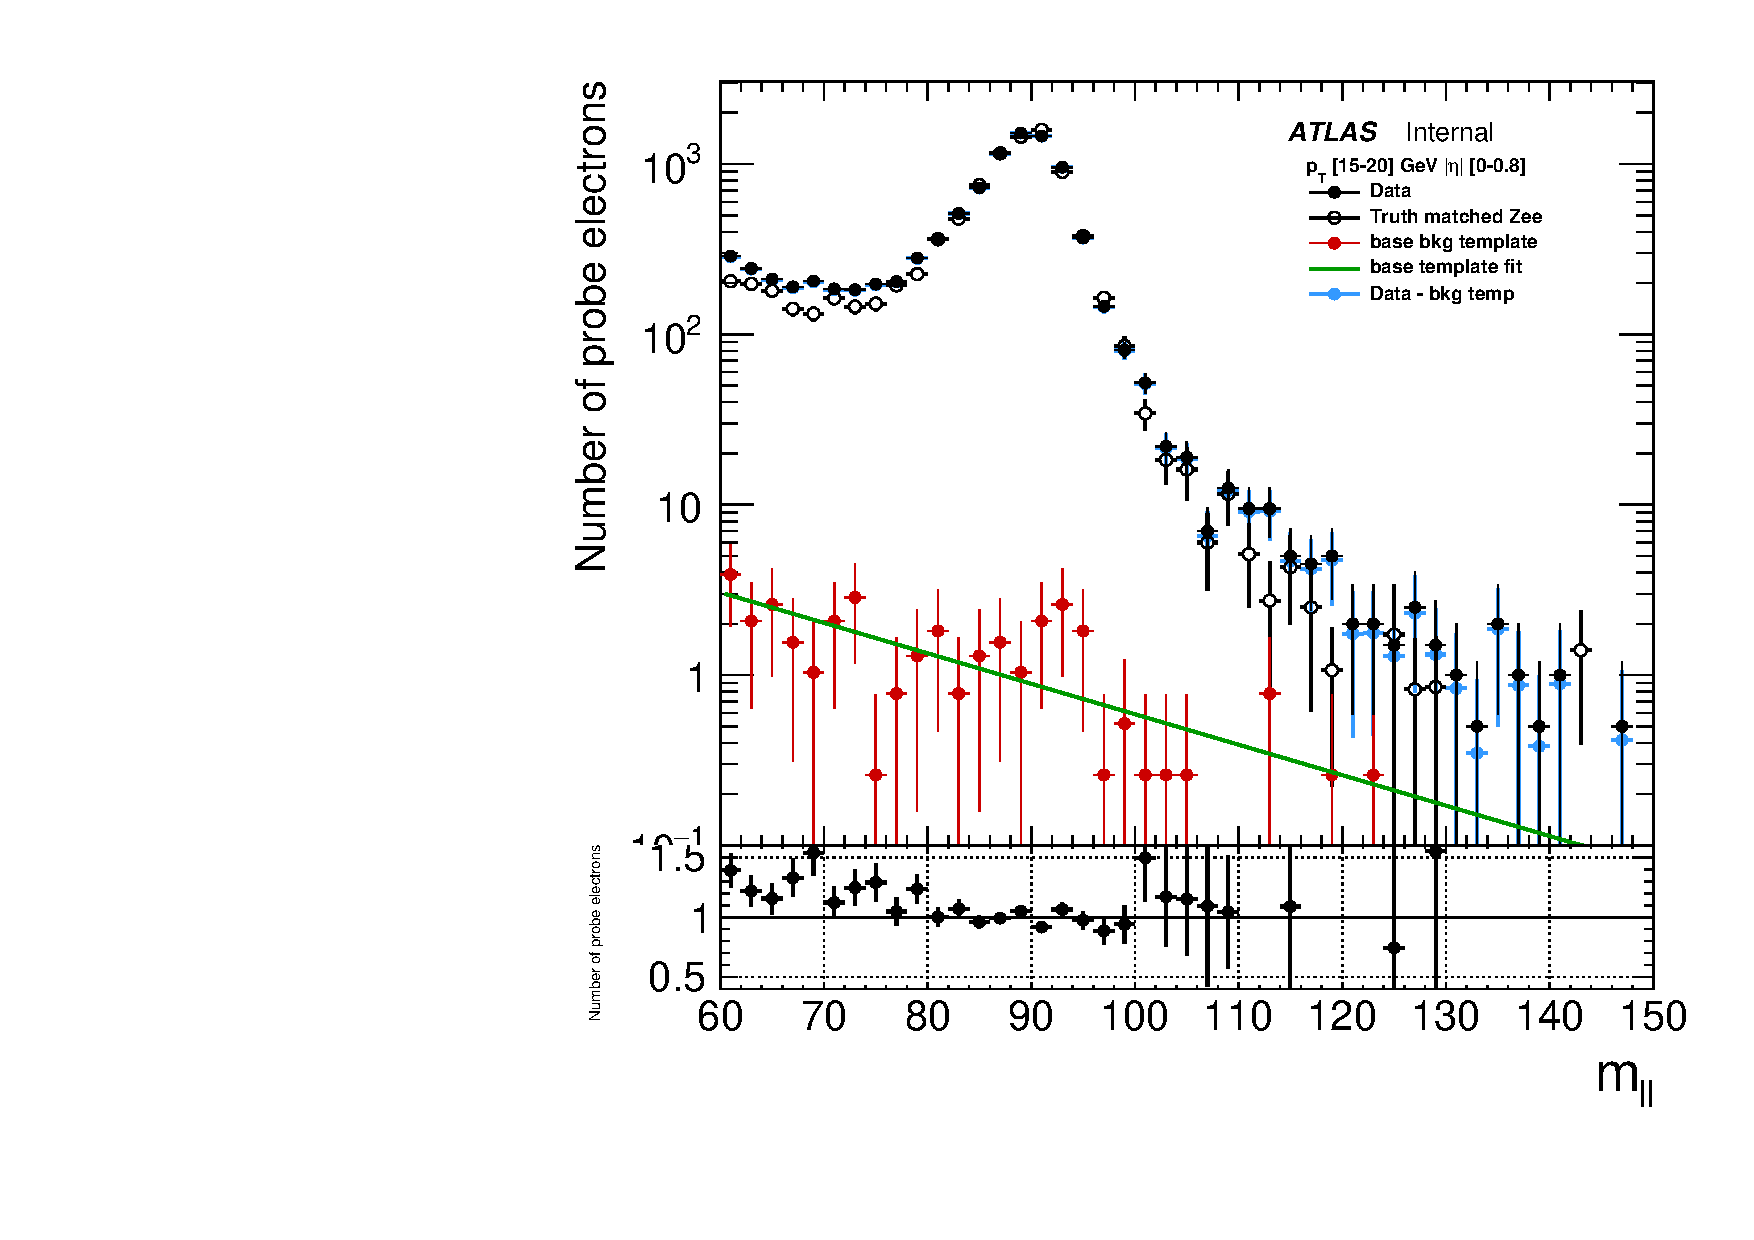
\includegraphics[width=0.30\textwidth]{BKG/realEff/Background_subtraction/Data_background_template_electrons_ZTandP_logScale_15_20_00_08_closure_test.pdf} 
	   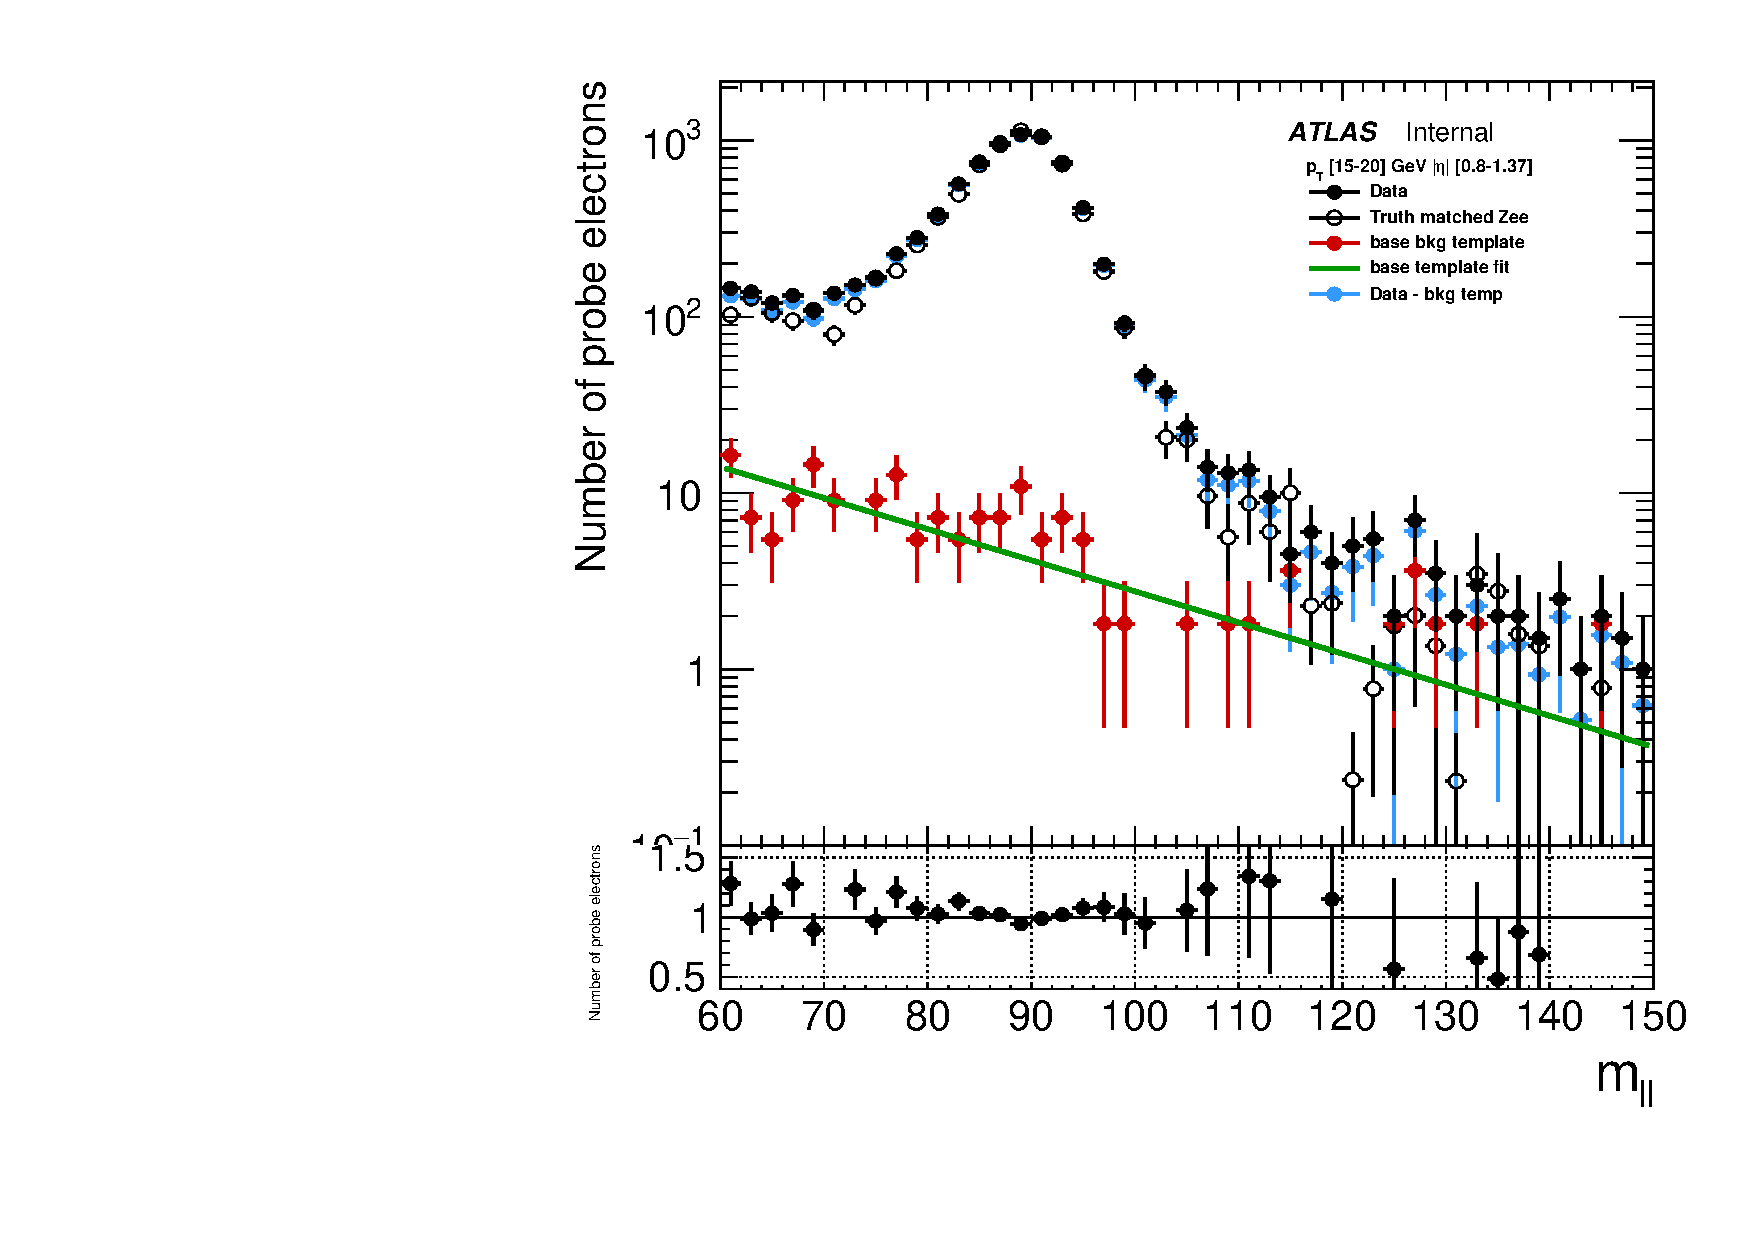
\includegraphics[width=0.30\textwidth]{BKG/realEff/Background_subtraction/Data_background_template_electrons_ZTandP_logScale_15_20_08_137_closure_test.pdf} 
	   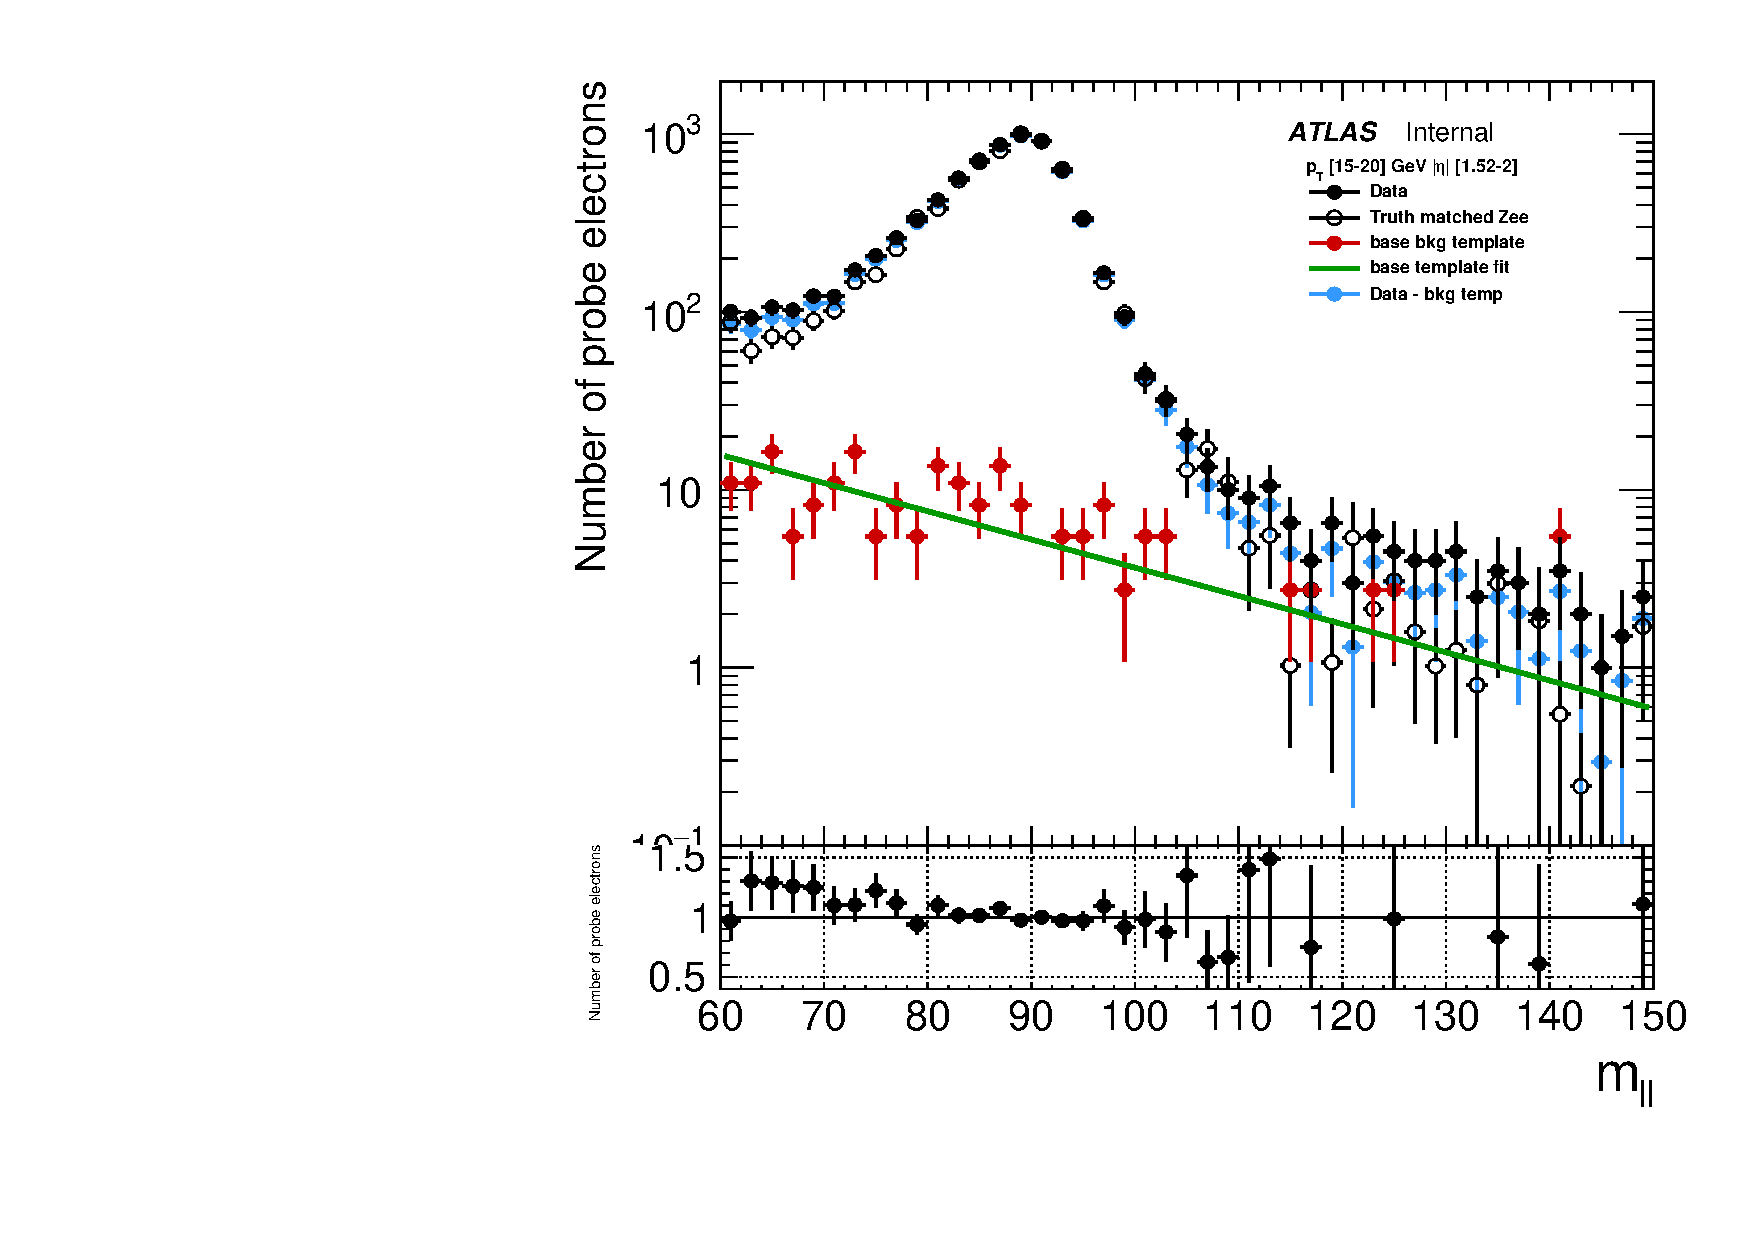
\includegraphics[width=0.30\textwidth]{BKG/realEff/Background_subtraction/Data_background_template_electrons_ZTandP_logScale_15_20_152_20_closure_test.pdf}
	   \caption{\label{fig:bkg_templates_closure} Plots illustrating the background subtraction procedure. The top (bottom) plots corresponds to the [10-15] ([15-20]) GeV \pt range and the left, medium and right ones to the [0-0.8], [0.8-1.37] and [1.52-2] $|\eta|$ range respectively. The $m_{\ell\ell}$ distributions from data (full points) before (black) and after (blue) background subtraction are shown along with the corresponding Monte Carlo distributions (open points). The Monte Carlo distribution is normalized to the data after background subtraction using a Gaussian fit of the $Z$ peak region. The ratio corresponds to the comparisons of the data (after background subtraction) with the Monte Carlo. The corresponding background templates (red) and their respective fit (green lines) are also shown.}
  \end{center}
\end{figure}				
%%%%%%%%%%%%%%%%%%%%%%%%%%%%%%%%%%%%%%%%%%%%%%%%%%%%%%%%%%%%


     
       \par{\bf Measurements systematics\\}
       A systematic uncertainty associated to the electron tag-and-probe measurement method has been set varying the background template definition, the template fit range and the $m_{\ell\ell}$ window used for the efficiency measurement. The variation of the templates definitions cuts are presented in table \ref{tab:efficiency_bkg_estimates} and the additional template fit ranges are the following : $[60-70]\cup[100-120]$ and $[65-75]\cup[100-120]$. The two other measurement $m_{\ell\ell}$ windows considered are the following : $[75-105]$ and $[85-95]$. In total 27 variations of the measurement method are considered in the $\pt < 20$ GeV range and 3 in the $\pt > 20$ GeV range. The largest contribution to the systematic uncertainties arises from the $m_{\ell\ell}$ window variations. This result is expected as electrons extracted from the lower $m_{\ell\ell}$ tail are affected by bremsstrahlung effects. Thus, the efficiency computed with electrons extracted with a large $m_{\ell\ell}$ window will be lower than the ones computed using a tight window. In the $10 < \pt < 15$ GeV range, the order of magnitude of the $m_{\ell\ell}$ window variation is $6\%$ whereas the background subtraction one is $1\%$. This result shows the robustness of the background subtraction method.\\
       The track isolation efficiency requirement used in the signal muons definitions has been measured by the muon CP group using a very similar method. As the real muon efficiency is fully dominated by the track isolation cut (see top right plot from Figure \ref{fig:CutEff_MC}), the systematic uncertainties associated to the efficiency measurement of this cut is used to asses the measurement systematic of the muons.


       \par{\bf Data to Monte Carlo comparisons\\}
       In this section, for information only (only the data measurements are used for the fake estimates) real lepton efficiencies computed with the $Z$ tag-and-probe method in data are compared to the ones using simulated $Z\rightarrow \ell\ell$ processes. All 2015 run~2 data is considered which corresponds to an integrated luminosity of $\sim3.2~\mathrm{fb}^{-1}$ after good run list requirements. All the Monte Carlo lepton scale factors provided by the CP group are applied and the simulation is reweighed to the pile-up observed in data. Besides, an additional loose truth match is added for the Monte Carlo lepton selection.
			
	% Real efficiencies Vs pt		
	The left plots from Figure \ref{fig:Data_Vs_MC_Real_Eff} shows the electron (top) and the muon (bottom) real leptons efficiencies as a function of $\pt$ measured on data and with simulated $Z\rightarrow ee$ and $Z\rightarrow\mu\mu$ processes. The associated uncertainties corresponds to the quadratic sum of the statistical and the measurement systematic uncertainties. The statistical uncertainties take both the background subtraction statistical uncertainties and the ones from the measurements into account\footnote{The measurement statistic uncertainties are driven by the statistical fluctuations in the [80-100] $m_{\ell\ell}$ range and the background subtraction ones by the fluctuations in the [120-150] GeV range where the background template normalisation is estimated.}. A reasonable data to Monte Carlo agreement is observed with $\sim2\%$ real efficiencies differences in the $\pt < 40$ GeV range and within the percent level in the $\pt > 40$ GeV range. These differences are covered by the measurement systematic uncertainties. The real muon efficiencies computed on Monte Carlo agree with the ones computed on data within $2\%$ in the $\pt <$ 20 GeV range, within the percent level in the $20 < \pt < 35$ GeV range and smaller than $0.5\%$ in the $\pt > 35$ GeV range.
				 
				 
%% MC to Data RealEfficiency comparisons
%%%%%%%%%%%%%%%%%%%%%%%%%%%%%%%%%%%%%%%%%%%%%%%%%%%%%%%%%%%%	
	\begin{figure}[!htb]
	  \begin{center} 
	   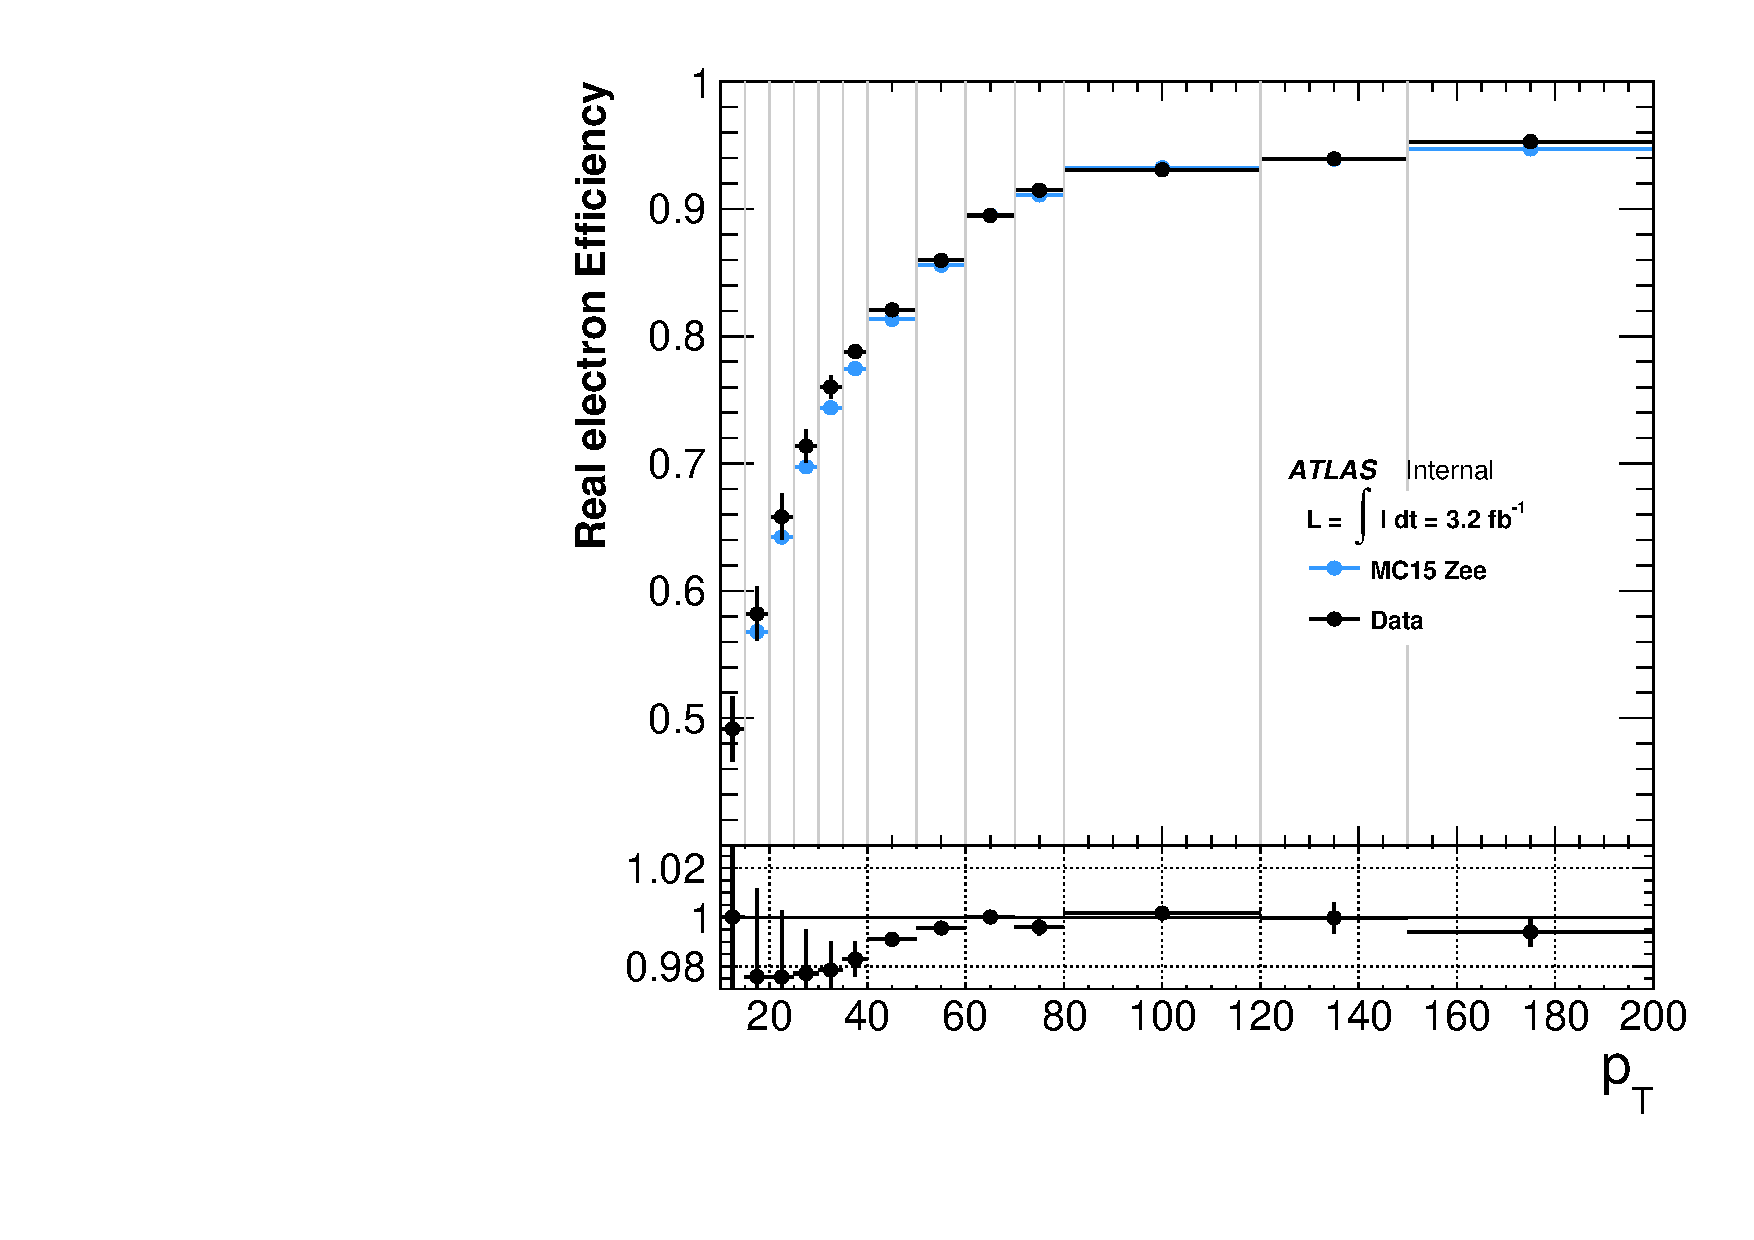
\includegraphics[width=0.3\textwidth]{BKG/realEff/Data_To_MC/Data_Vs_MC15_RealEfficiencies_Vs_pt_electrons_ZTandP.pdf} 
	   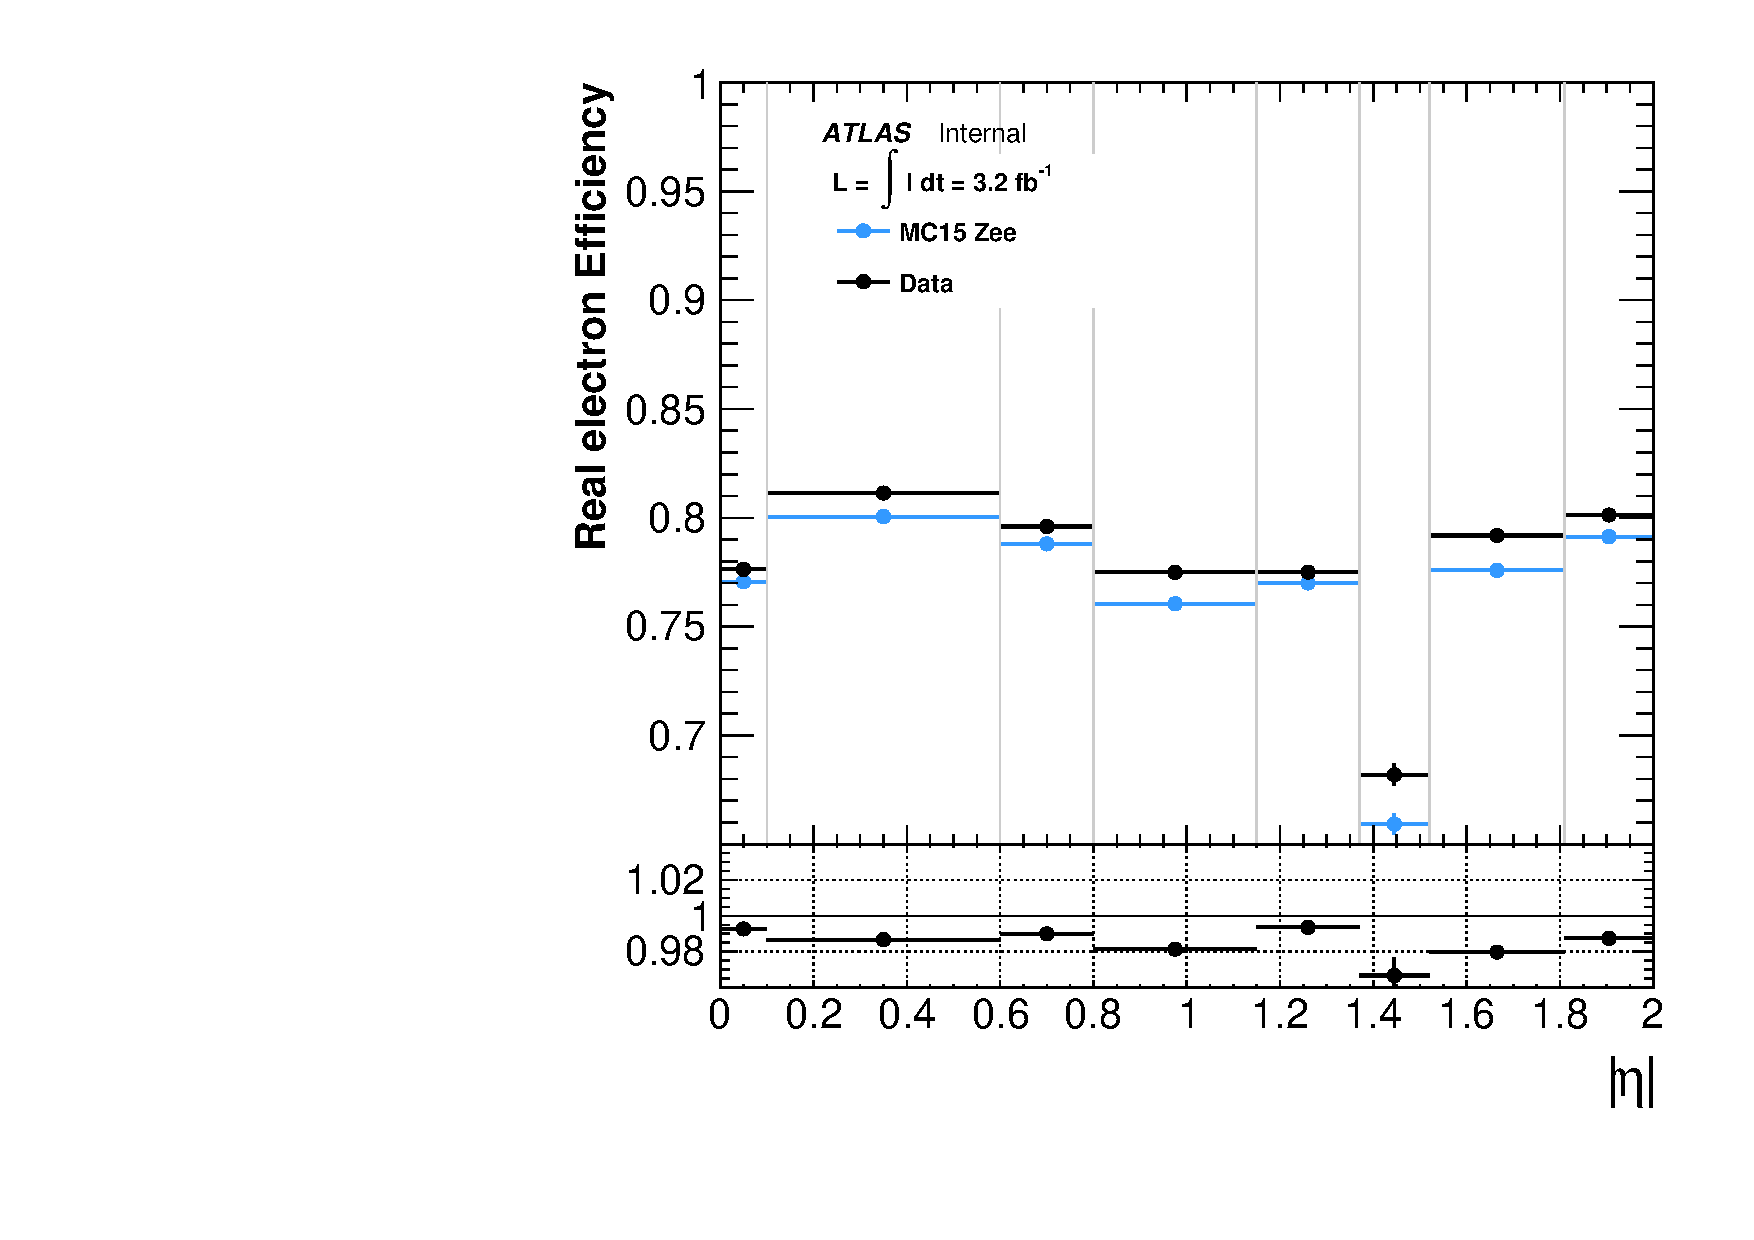
\includegraphics[width=0.3\textwidth]{BKG/realEff/Data_To_MC/Data_Vs_MC15_RealEfficiencies_Vs_eta_electrons_ZTandP.pdf} 
	   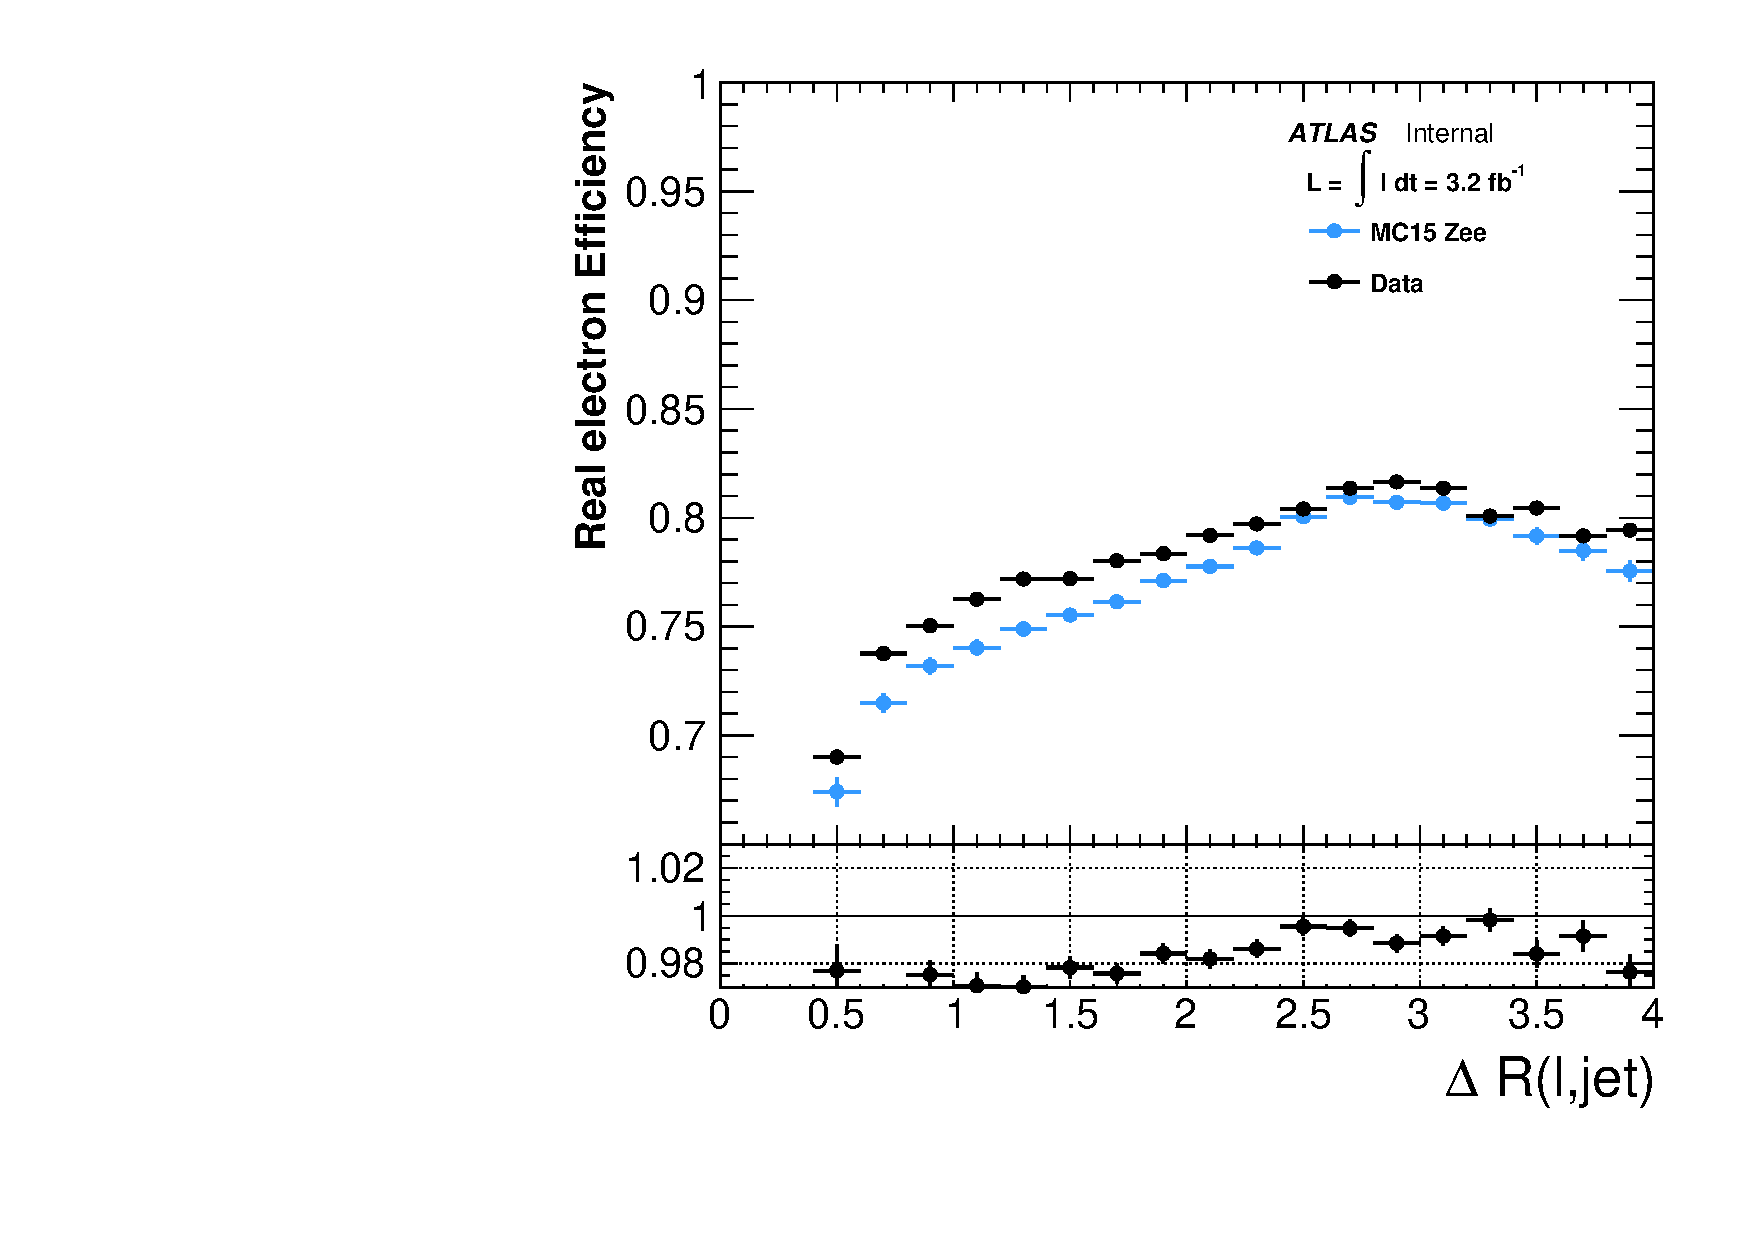
\includegraphics[width=0.3\textwidth]{BKG/realEff/Data_To_MC/Data_Vs_MC15_RealEfficiencies_Vs_DRjet_electrons_ZTandP.pdf} 
	   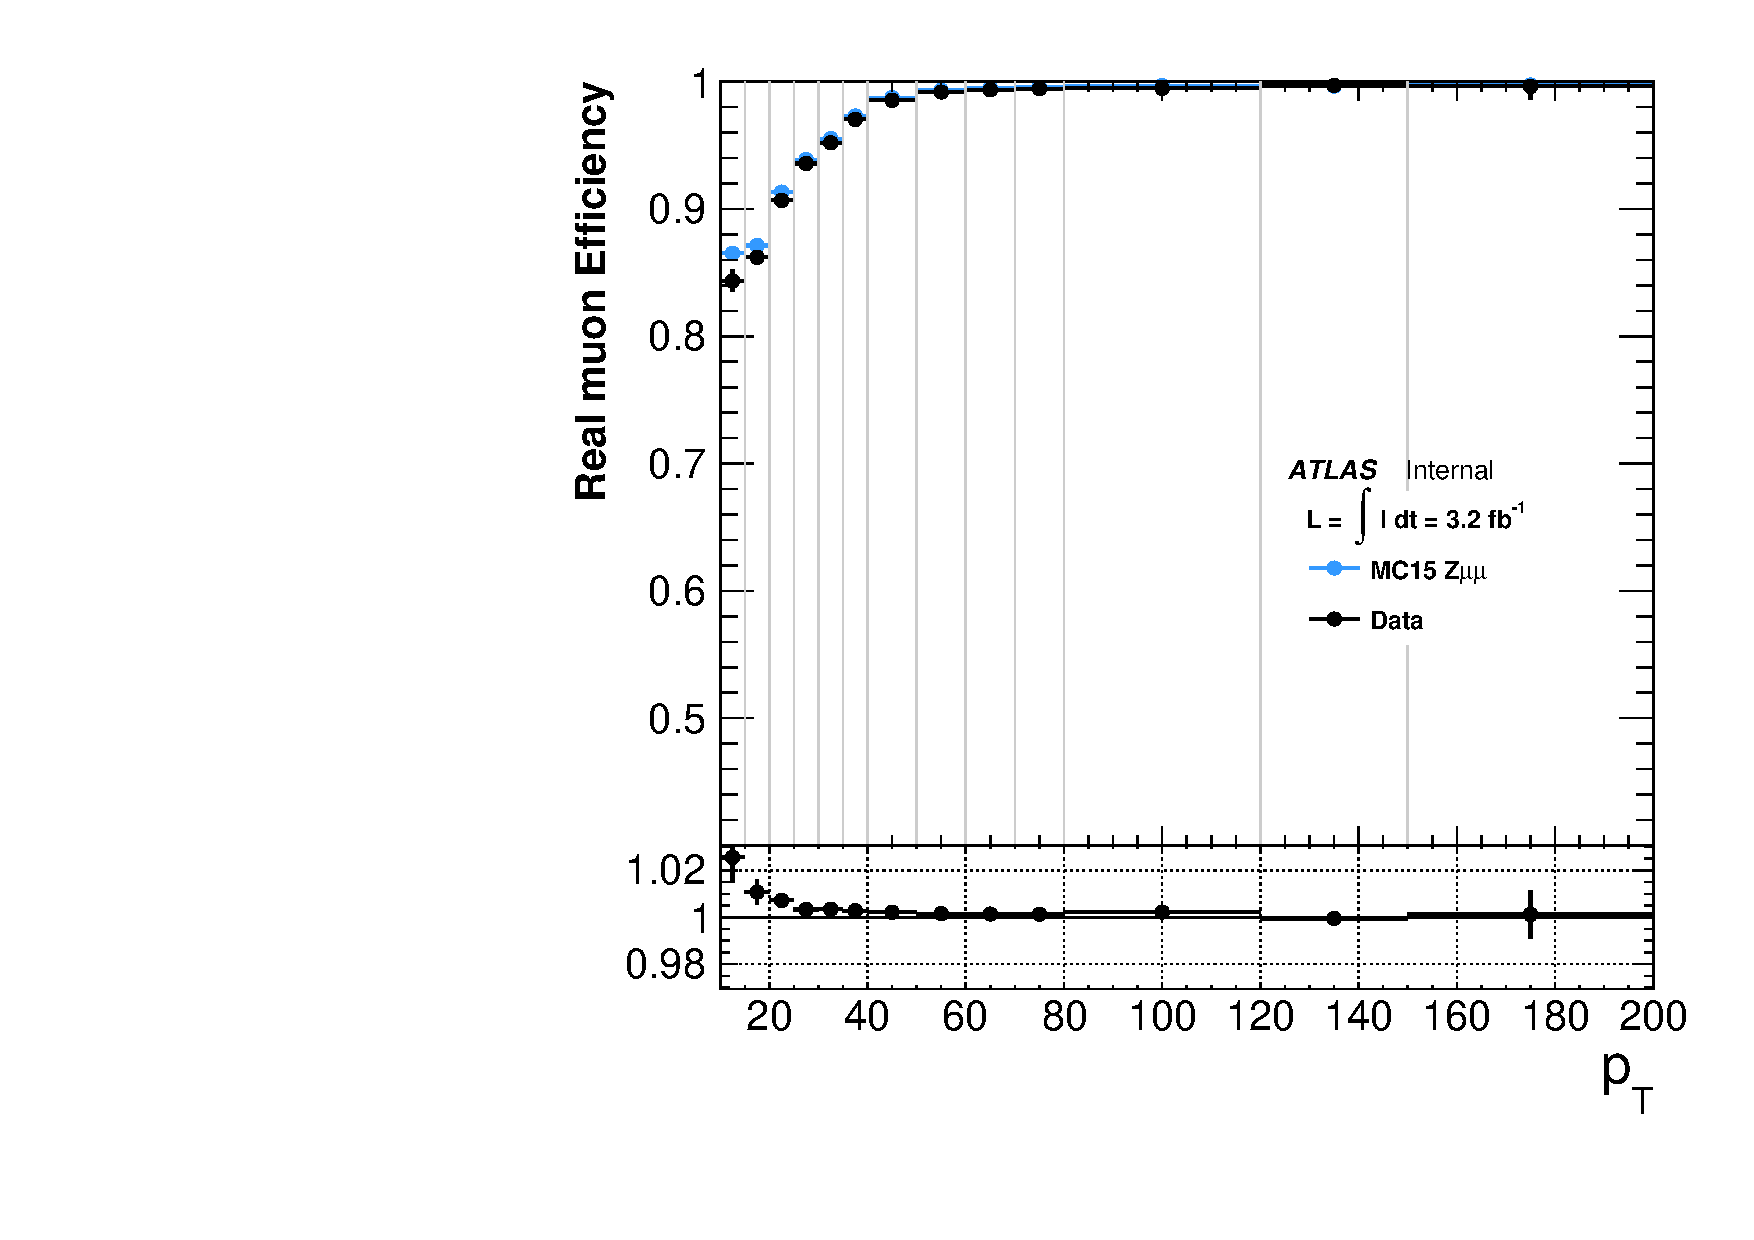
\includegraphics[width=0.3\textwidth]{BKG/realEff/Data_To_MC/Data_Vs_MC15_RealEfficiencies_Vs_pt_muons_ZTandP.pdf} 	
	   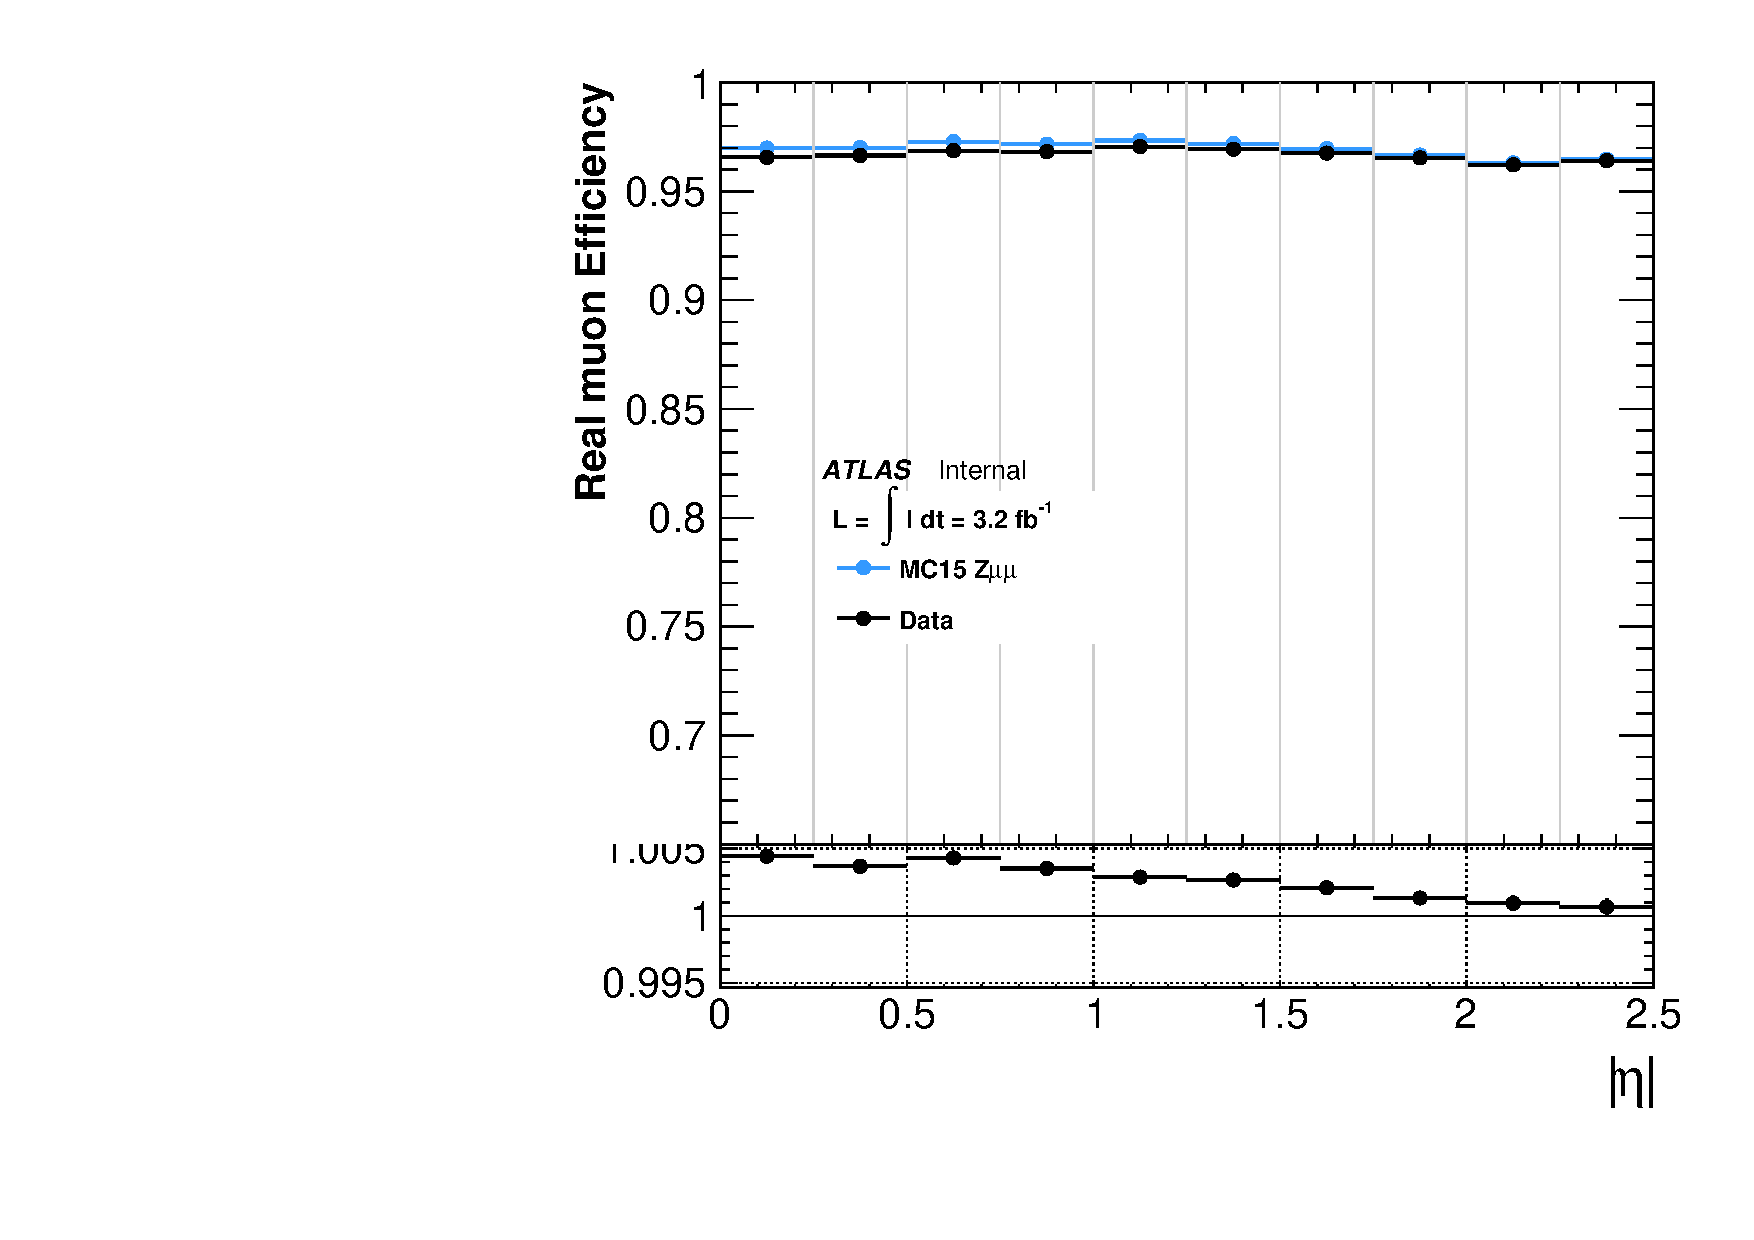
\includegraphics[width=0.3\textwidth]{BKG/realEff/Data_To_MC/Data_Vs_MC15_RealEfficiencies_Vs_eta_muons_ZTandP.pdf}
	   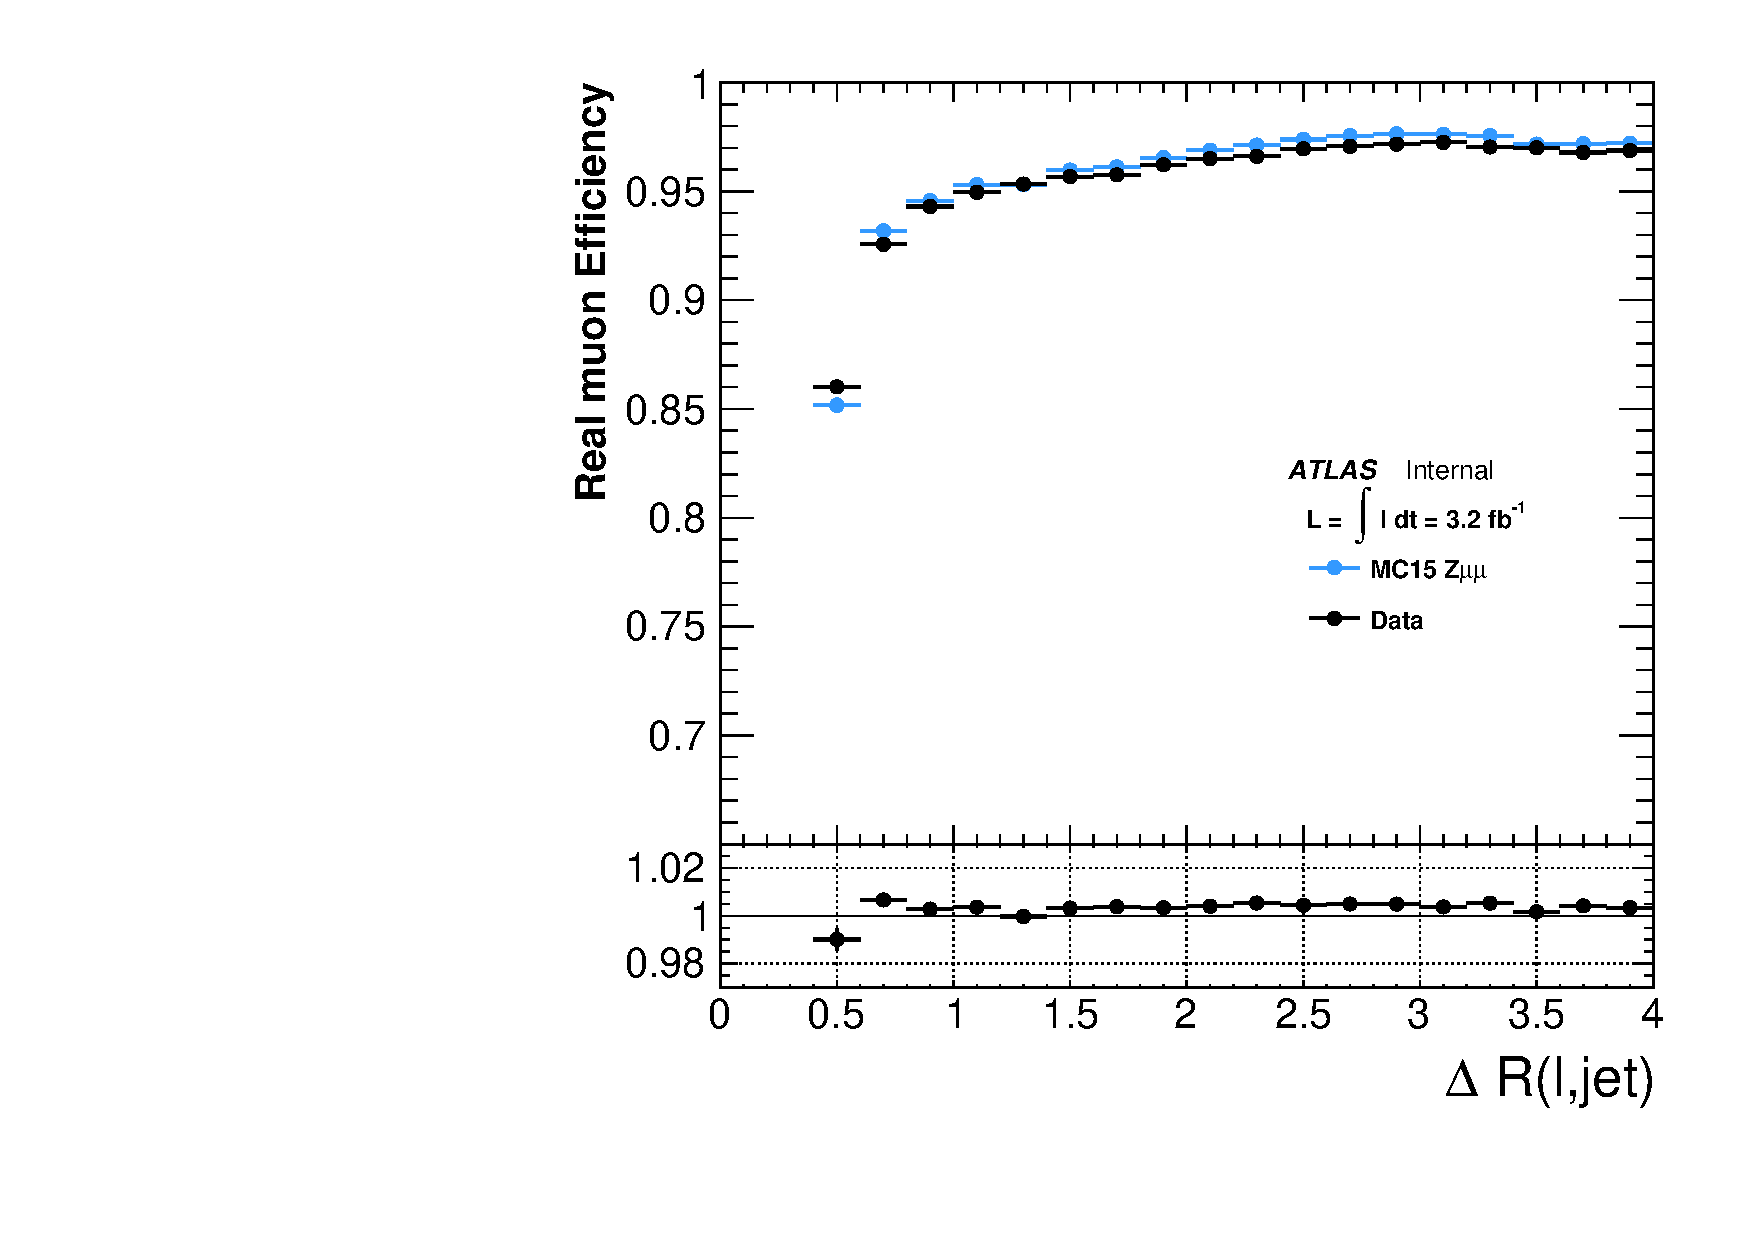
\includegraphics[width=0.3\textwidth]{BKG/realEff/Data_To_MC/Data_Vs_MC15_RealEfficiencies_Vs_DRjet_muons_ZTandP.pdf}
	   \caption{\label{fig:Data_Vs_MC_Real_Eff} Real lepton efficiencies as a function of lepton $p_{T}$ (left), $\eta$ (middle) and $\Delta R(\ell,Jet)$ (right) measured using the $Z$ tag-and-probe method described bellow. The top (bottom) plot corresponds to the electron (muon) real efficiencies. The black points corresponds to the efficiency computed using 2015 data. The blue points corresponds to the real leptons efficiency computed using $Z\rightarrow \ell\ell$ simulated events with lepton loose truth match reweighed to the data pile-up. The uncertainties shown in the left plots corresponds to the quadratic sum of the statistical and the measurement method uncertainties, whereas only statistical uncertainties are shown in the middle and the right plots. The binning used for the electron real efficiency measurement as a function of $\eta$ corresponds to the geometry of the electromagnetic calorimeter.}
	  \end{center}
	\end{figure}	
%%%%%%%%%%%%%%%%%%%%%%%%%%%%%%%%%%%%%%%%%%%%%%%%%%%%%%%%%%%%	
	
	% Real efficiencies Vs eta		
	The middle plots from Figure \ref{fig:Data_Vs_MC_Real_Eff} shows the electron (top) and the muon (bottom) real efficiencies as a function of $|\eta|$ measured using data and Monte Carlo. The shown errors corresponds to the statistics only. The efficiencies computed on Monte Carlo are $2\%$ lower that the data ones, which corresponds to the efficiencies differences observed in the 40 GeV \pt range that dominates the statistics. The muon efficiencies agree within $0.5\%$ and improves at high $|\eta|$.
        % Real efficiencies Vs DRjet
	The right plots from Figure \ref{fig:Data_Vs_MC_Real_Eff} shows the electron (top) and the muon (bottom) real efficiencies as a function of $\Delta R(l,jets)$ measured on data and Monte Carlo. The Data and Monte Carlo real electron efficiencies agree within $2\%$, whereas the muon real efficiencies agrees within the percent level.
	
	
\par{\bf Results\\}
	Figure \ref{fig:Real_Eff_Data_Vs_pt_eta} shows the leptons real efficiencies ($\epsilon$) computed as a function of $p_{T}$ and $\eta$ used by the the matrix method. The electron $\eta$ binning is driven the electromagnetic calorimeter geometry removing the crack region ($|\eta|[1.37-1.52]$) not considered in the analysis. The error bars show the quadratic sum of the statistic and the tag-and-probe measurement systematic uncertainties. 
				
%% Real letpton efficiency computed on Data
%%%%%%%%%%%%%%%%%%%%%%%%%%%%%%%%%%%%%%%%%%%%%%%%%%%%%%%%%%%%		
\begin{figure}[!htb]
  \begin{center} 
   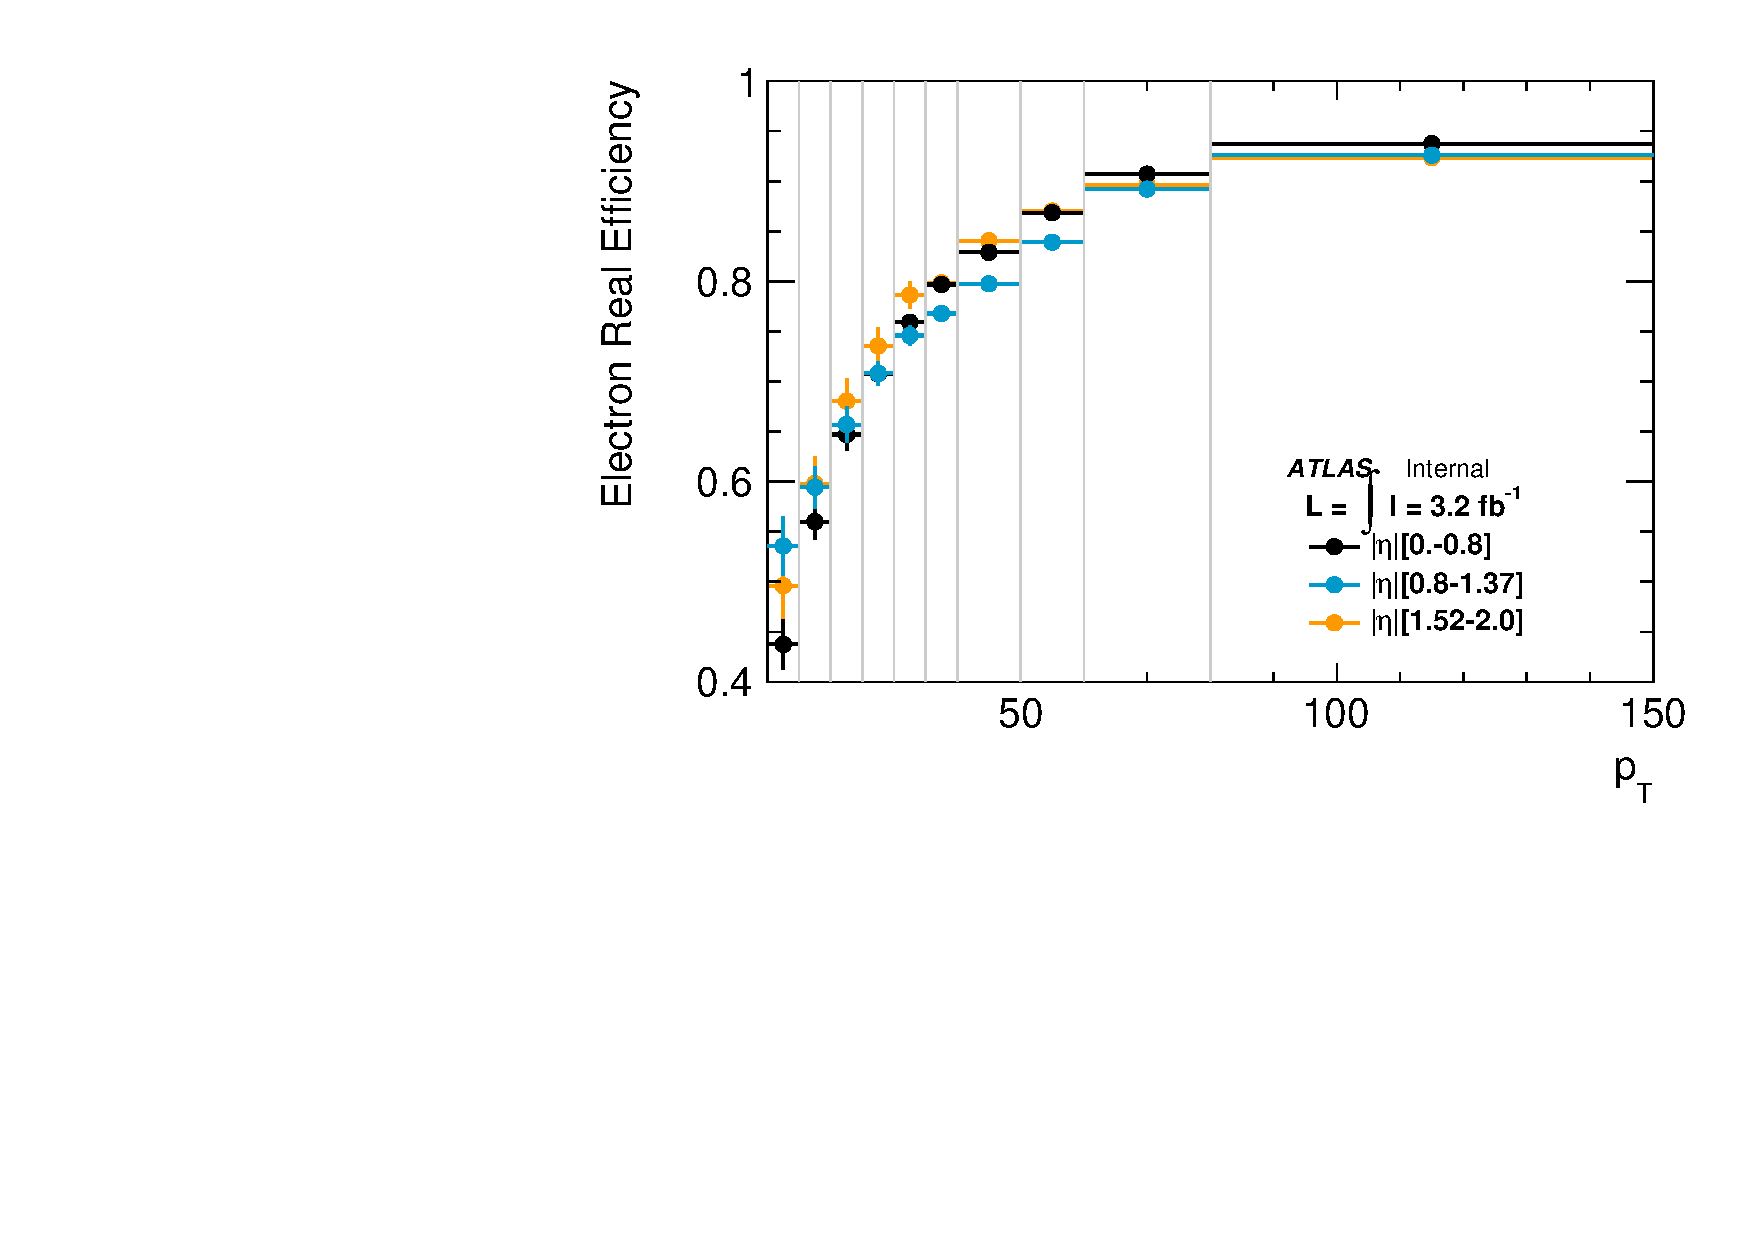
\includegraphics[width=0.45\textwidth]{BKG/realEff/Data_To_MC/Data_MergedData_RealEfficiencies_Vs_pt_eta_electrons_ZTandP.pdf} 
   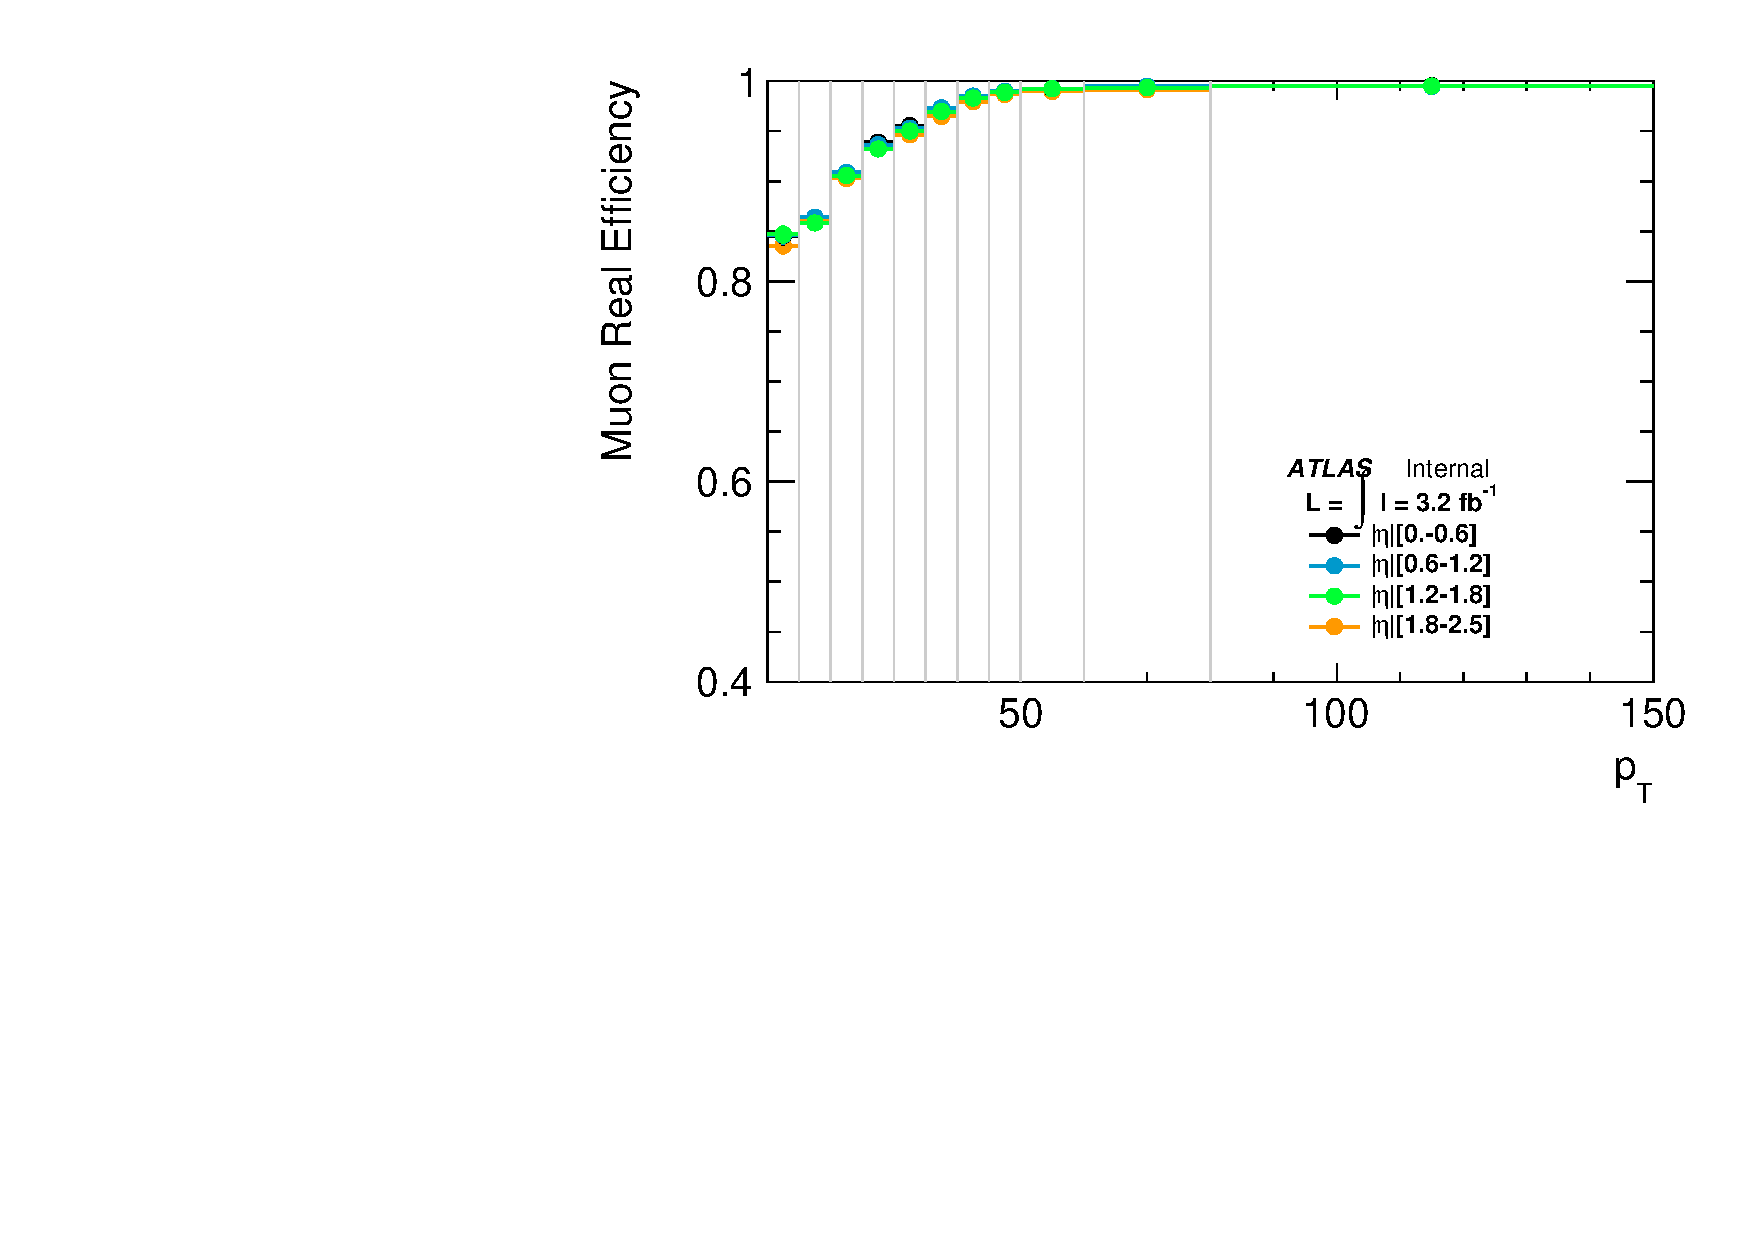
\includegraphics[width=0.45\textwidth]{BKG/realEff/Data_To_MC/Data_MergedData_RealEfficiencies_Vs_pt_eta_muons_ZTandP.pdf} 
   \caption{\label{fig:Real_Eff_Data_Vs_pt_eta} Real lepton efficiencies as a function of lepton $p_{T}$ and $\eta$ measured using the $Z$ tag-and-probe method described bellow. The left (right) plot corresponds to the electron (muon) real efficiencies. The binning used for the electron real efficiency measurement corresponds to the geometry of the electromagnetic calorimeter removing the calorimeter crack region (1.37 $< |\eta| <$ 1.52) and homogeneous $\eta$ binning has been chosen for the muons.}
  \end{center}
\end{figure}
%%%%%%%%%%%%%%%%%%%%%%%%%%%%%%%%%%%%%%%%%%%%%%%%%%%%%%%%%%%%	



%%%%%%%%%%%%%%%%%%
% SUBSECTION 3
%%%%%%%%%%%%%%%%%%
	\subsection{Z tag-and-probe systematics uncertainties}
	\label{App:RealEff_Z_Syst}
        Besides the systematics from the $Z$ tag-and-probe measurement other sources of systematics have been considered.
	
		\par{\bf Trigger systematics\\}
		Following the analysis trigger strategy, the electrons entering in the Signal Regions might be required to have fired one of the di-lepton triggers or not. For example if the event is fired with the $E_{\mathrm{T}}^{miss}$ trigger or if the considered lepton is the $3^{\mathrm{rd}}$ leading lepton, no trigger match should be applied for the efficiency computations. On the other hand, if the event is triggered by the di-lepton and the considered lepton is the leading or the sub-leading one, a trigger matching should be applied before the real lepton efficiency computation.
                Figure \ref{fig:Syst_Trigger_Dep} shows the real lepton efficiencies computed with and without the relevant real lepton trigger as a function of $\pt$. The right plot dedicated to the muon efficiencies show that the trigger strategy does not affect the muon efficiency measurement, whereas the left plot, dedicated to electrons shows a sizeable bias is induced by the di-electron trigger. As the di-electron trigger is using a 12 GeV $E_{\mathrm{T}}$ threshold, this bias is expected in the $10 < \pt < 15$ GeV range. The unexpected bias seen in the $\pt > 15$ GeV range is understood to be due to the $\texttt{e12\_lhloose}$ trigger inefficiencies reported by the egamma trigger group. As the real lepton efficiencies are measured with events triggered by a single lepton trigger\footnote{The tag is matched to the single lepton trigger in order to provide unbiased probe leptons for the efficiency measurements.}, an additional systematic is assigned as the differences between the efficiencies measured with leptons matched with the $\texttt{e12\_lhloose}$ trigger and the lepton without trigger match. Moreover as a $\pt > 20$ GeV requirement is applied on the two leading leptons, the leptons with $\pt < 20$ will never be trigger matched to the di-lepton trigger. Therefore no systematics is assigned in the $10 < \pt < 20$ GeV range. A relative systematic uncertainty of $4\%$ is assigned to electrons in the $20 < \pt < 30$ GeV range, $2\%$ in the $30 < \pt < 50$ GeV range, $1\%$ in the $50 < \pt < 60$ GeV range and $0.5\%$ for electrons in the $\pt > 60$ GeV range.
					
%%%%%%%%%%%%%%%%%%%%%%%%%%%%%%%%%%%%%%%%%%%%%%%%%%%%%%%%%%%%	
	\begin{figure}[!h]
	  \begin{center} 
	   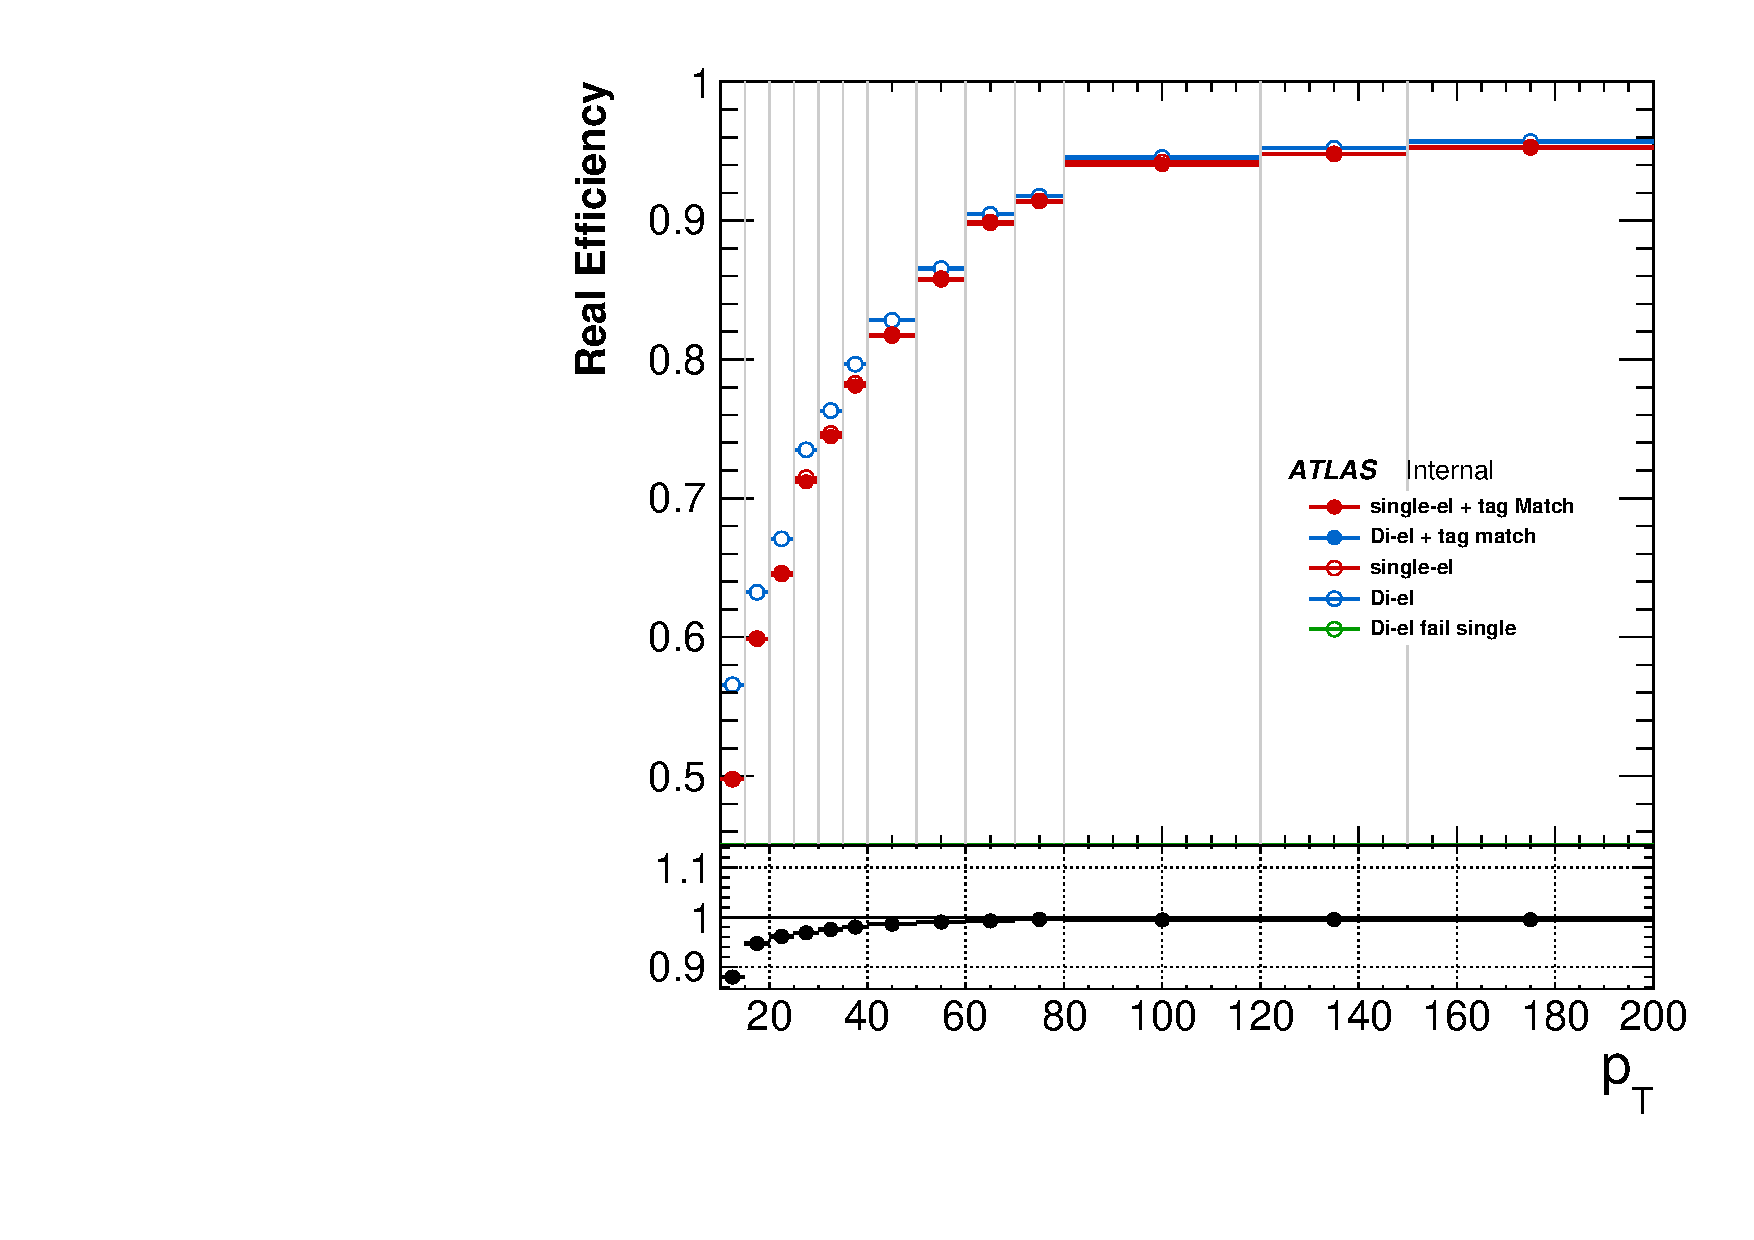
\includegraphics[width=0.4\textwidth]{BKG/realEff/Syst/Trigger_MC_RealEfficiencies_Vs_ptelectrons_ZTandP.pdf} 
	   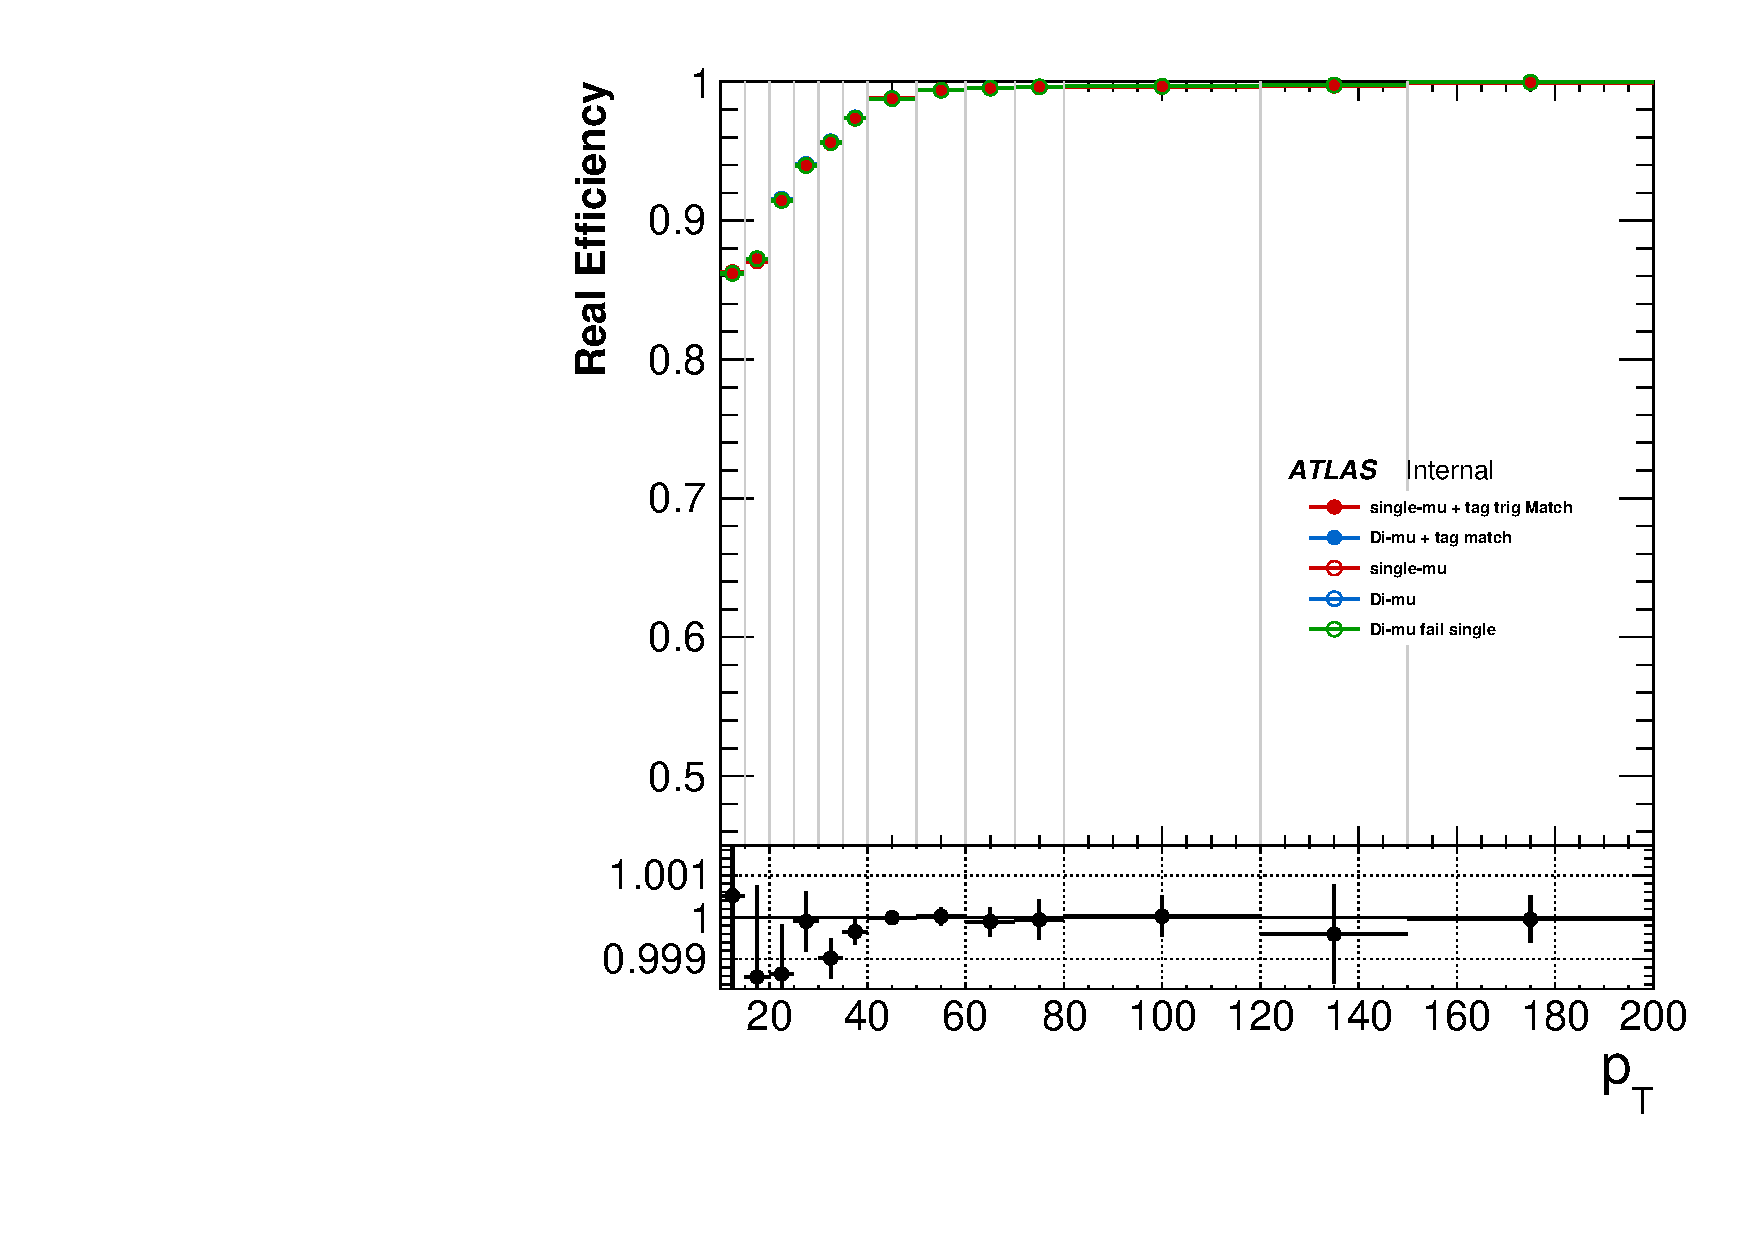
\includegraphics[width=0.4\textwidth]{BKG/realEff/Syst/Trigger_MC_RealEfficiencies_Vs_ptmuons_ZTandP.pdf}
	   \caption{\label{fig:Syst_Trigger_Dep} Real electron (left) and muon (right) efficiency computed with and without di-lepton trigger applied using $Z\rightarrow ll$ simulated events. The full dots shows the real lepton efficiencies computed with a trigger match on the tag lepton and the open ones correspond to the efficiencies computed with a Z tag-and-probe method with trigger match on the tag lepton. The blue points correspond to the efficiency measurements with the di-lepton trigger and the red ones with the single lepton trigger only. As only $Z\rightarrow ll$ events with two baseline leptons are used to compute these efficiencies, applying the di-lepton trigger is equivalent to match the probe lepton to the $e12\_lhloose$ lepton trigger.}
	  \end{center}
	\end{figure}	
%%%%%%%%%%%%%%%%%%%%%%%%%%%%%%%%%%%%%%%%%%%%%%%%%%%%%%%%%%%%	
		
	\par{\bf SUSY signal topology extrapolation systematics\\}
	The real lepton efficiencies are measured with a sample enriched in $Z\rightarrow ll$ events characterized by well isolated leptons. The different processes entering in the signal region are accompanied by many (b)jets and with a different event topology\footnote{Some SUSY processes can lead to events with very boosted top quarks reducing the angular distance between the physical objects.}. Thus, the leptons present in the final state are not necessary well isolated. As tight isolation cuts are used for the signal lepton definitions, their associated real efficiency can be smaller. These potential efficiencies differences are assigned as a systematic uncertainty by comparing the real lepton efficiencies computed with $Z\rightarrow ll$ processes and the ones computed considering several SUSY benchmark model : $\tilde{g}\tilde{g} \rightarrow t\overline{t}t\overline{t} \tilde{\chi}^0_1 \tilde{\chi}^0_1$. Boosted topologies are selected by applying the following requirement to select the models $m_{\tilde{g}} - m_{\tilde{\chi}^0_1} > 1000$ GeV. As the topology of one of the main irreducible backgrounds $t\overline{t}V$ is close to the $t\overline{t}$ one, the efficiencies measured with leptons from $t\overline{t}$ are also considered. The efficiencies comparisons are made for each measurements \pt bins considering two $\Delta R(\ell,\mathrm{Jets})$ ranges : [0.4-0.6] and $\Delta R(\ell,\mathrm{Jets}) > 0.6$. The obtained efficiencies ratios are then used to define the systematics.\\
	Figure \ref{fig:Syst_kinematics} shows kinematic distributions of the baseline truth matched leptons from the processes considered for the systematic study. The top and the bottom plots, dedicated to the lepton $\pt$ and $|\eta|$ distributions, show that the leptons from the SUSY process are more boosted and more central than the ones from $Z$ and $t\overline{t}$ processes.\\
	
%%%%%%%%%%%%%%%%%%%%%%%%%%%%%%%%%%%%%%%%%%%%%%%%%%%%%%%%%%%%	
	\begin{figure}[!h]
	  \begin{center} 
	   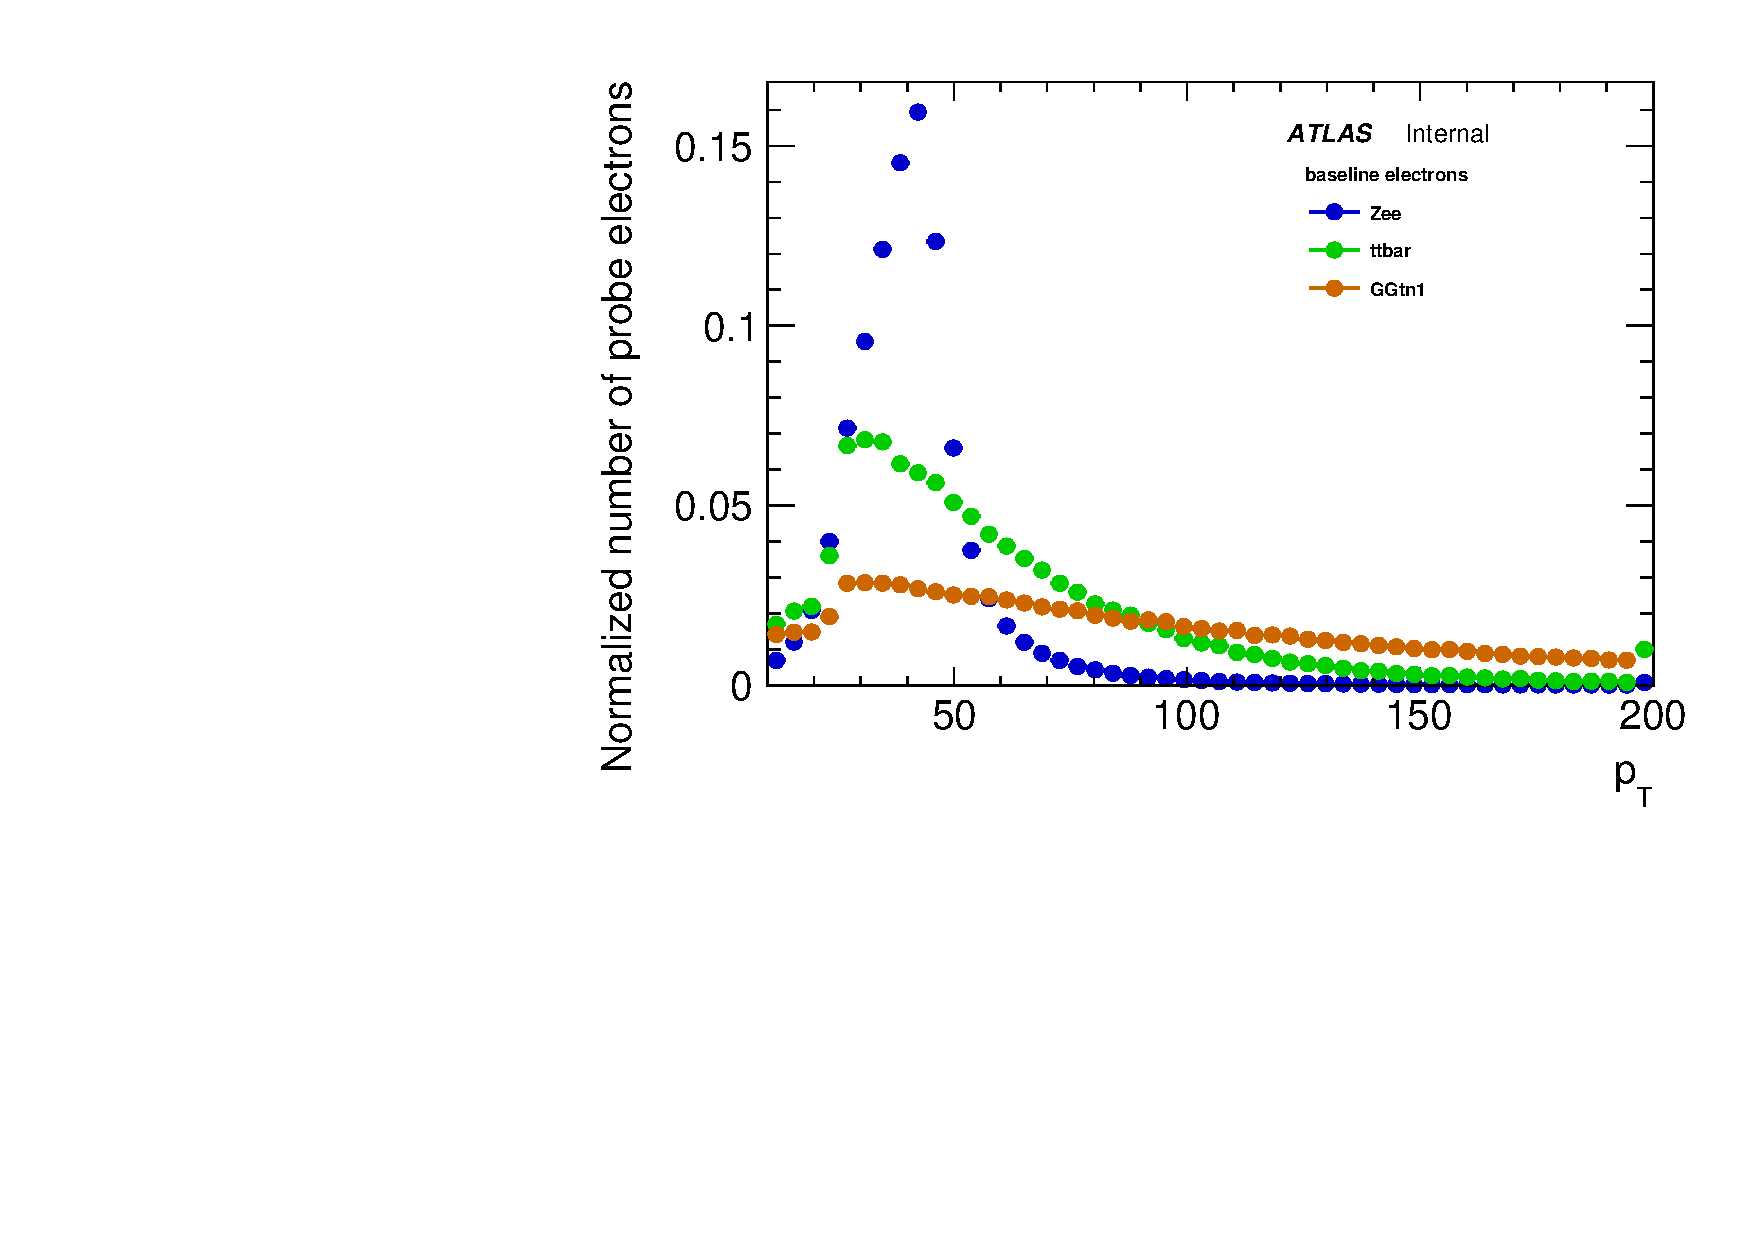
\includegraphics[width=0.4\textwidth]{BKG/realEff/Syst/Syst_Topo_baseline_pt_distribution_electrons.pdf} 
	   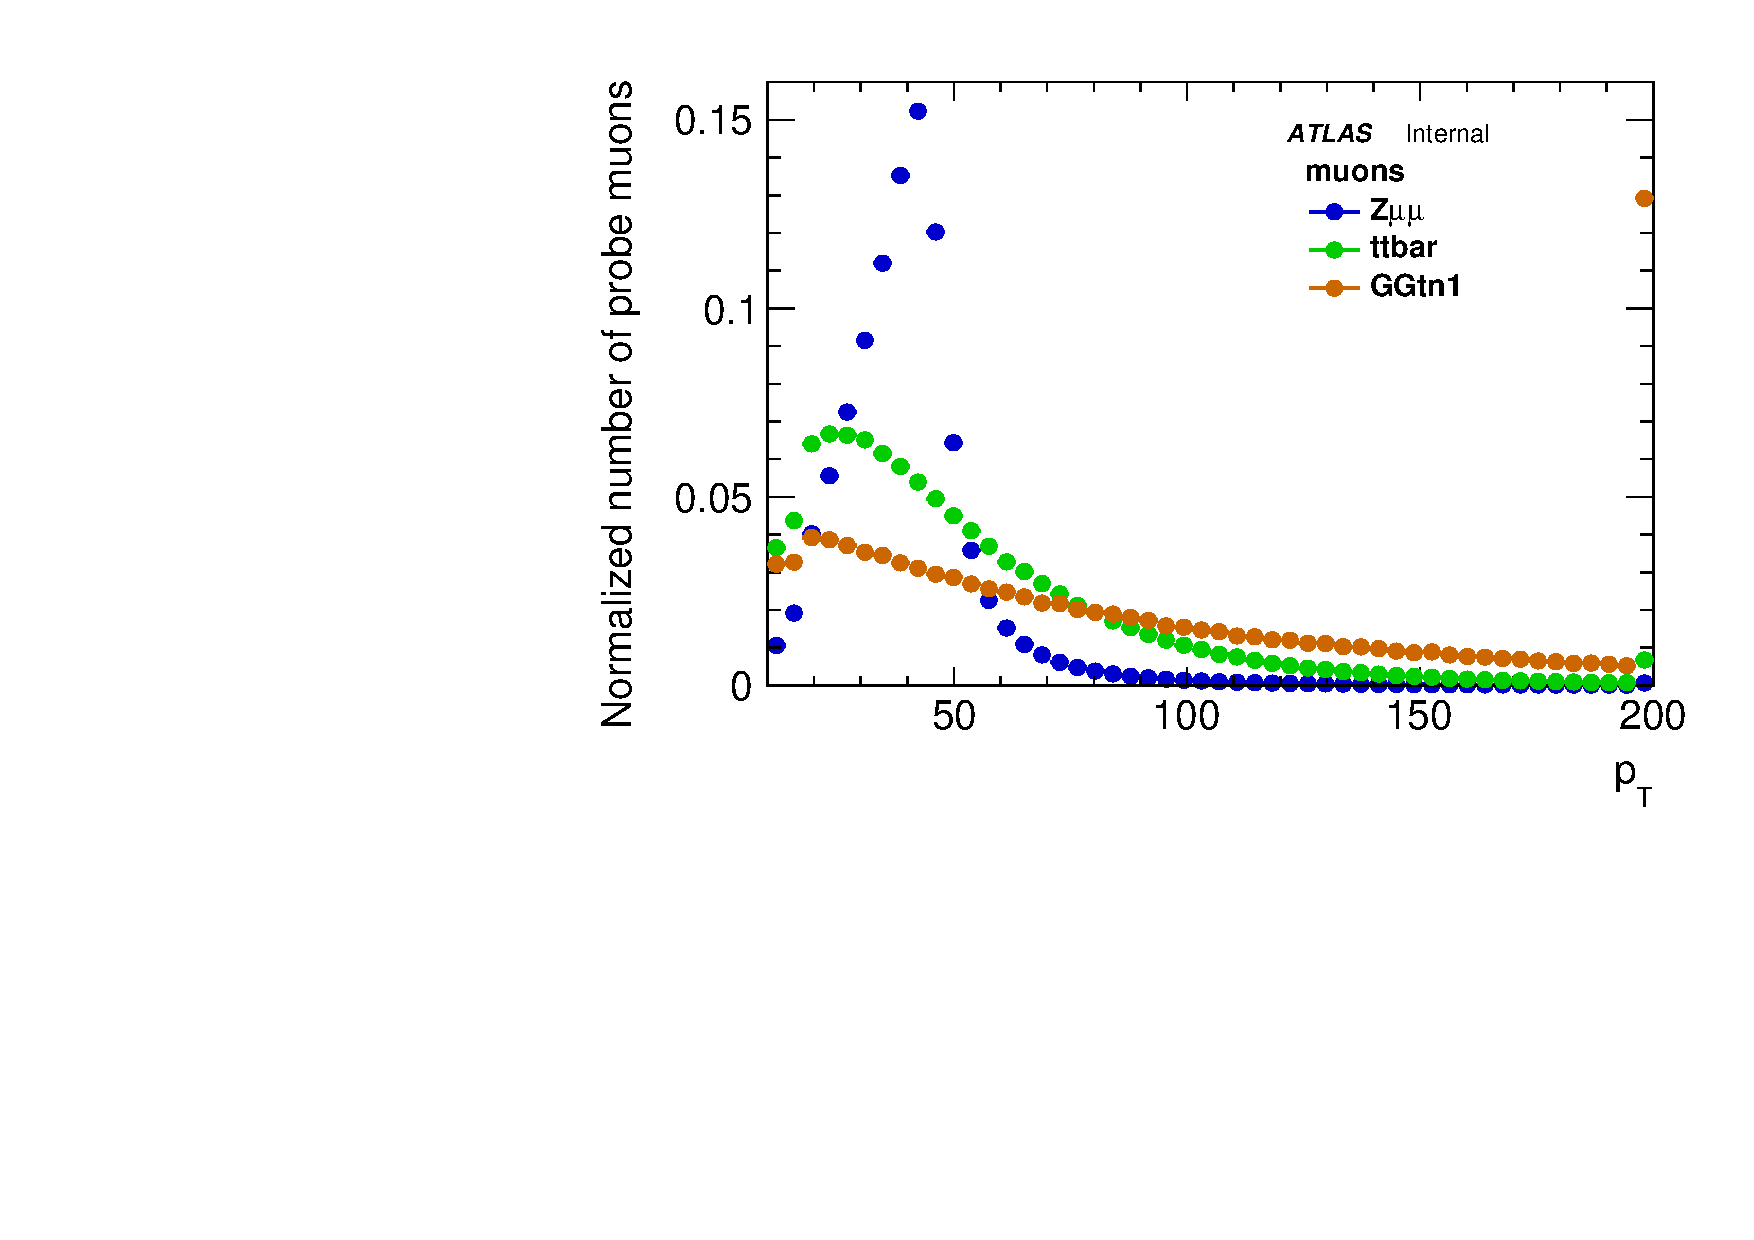
\includegraphics[width=0.4\textwidth]{BKG/realEff/Syst/Syst_Topo_baseline_pt_distribution_muons.pdf}
	   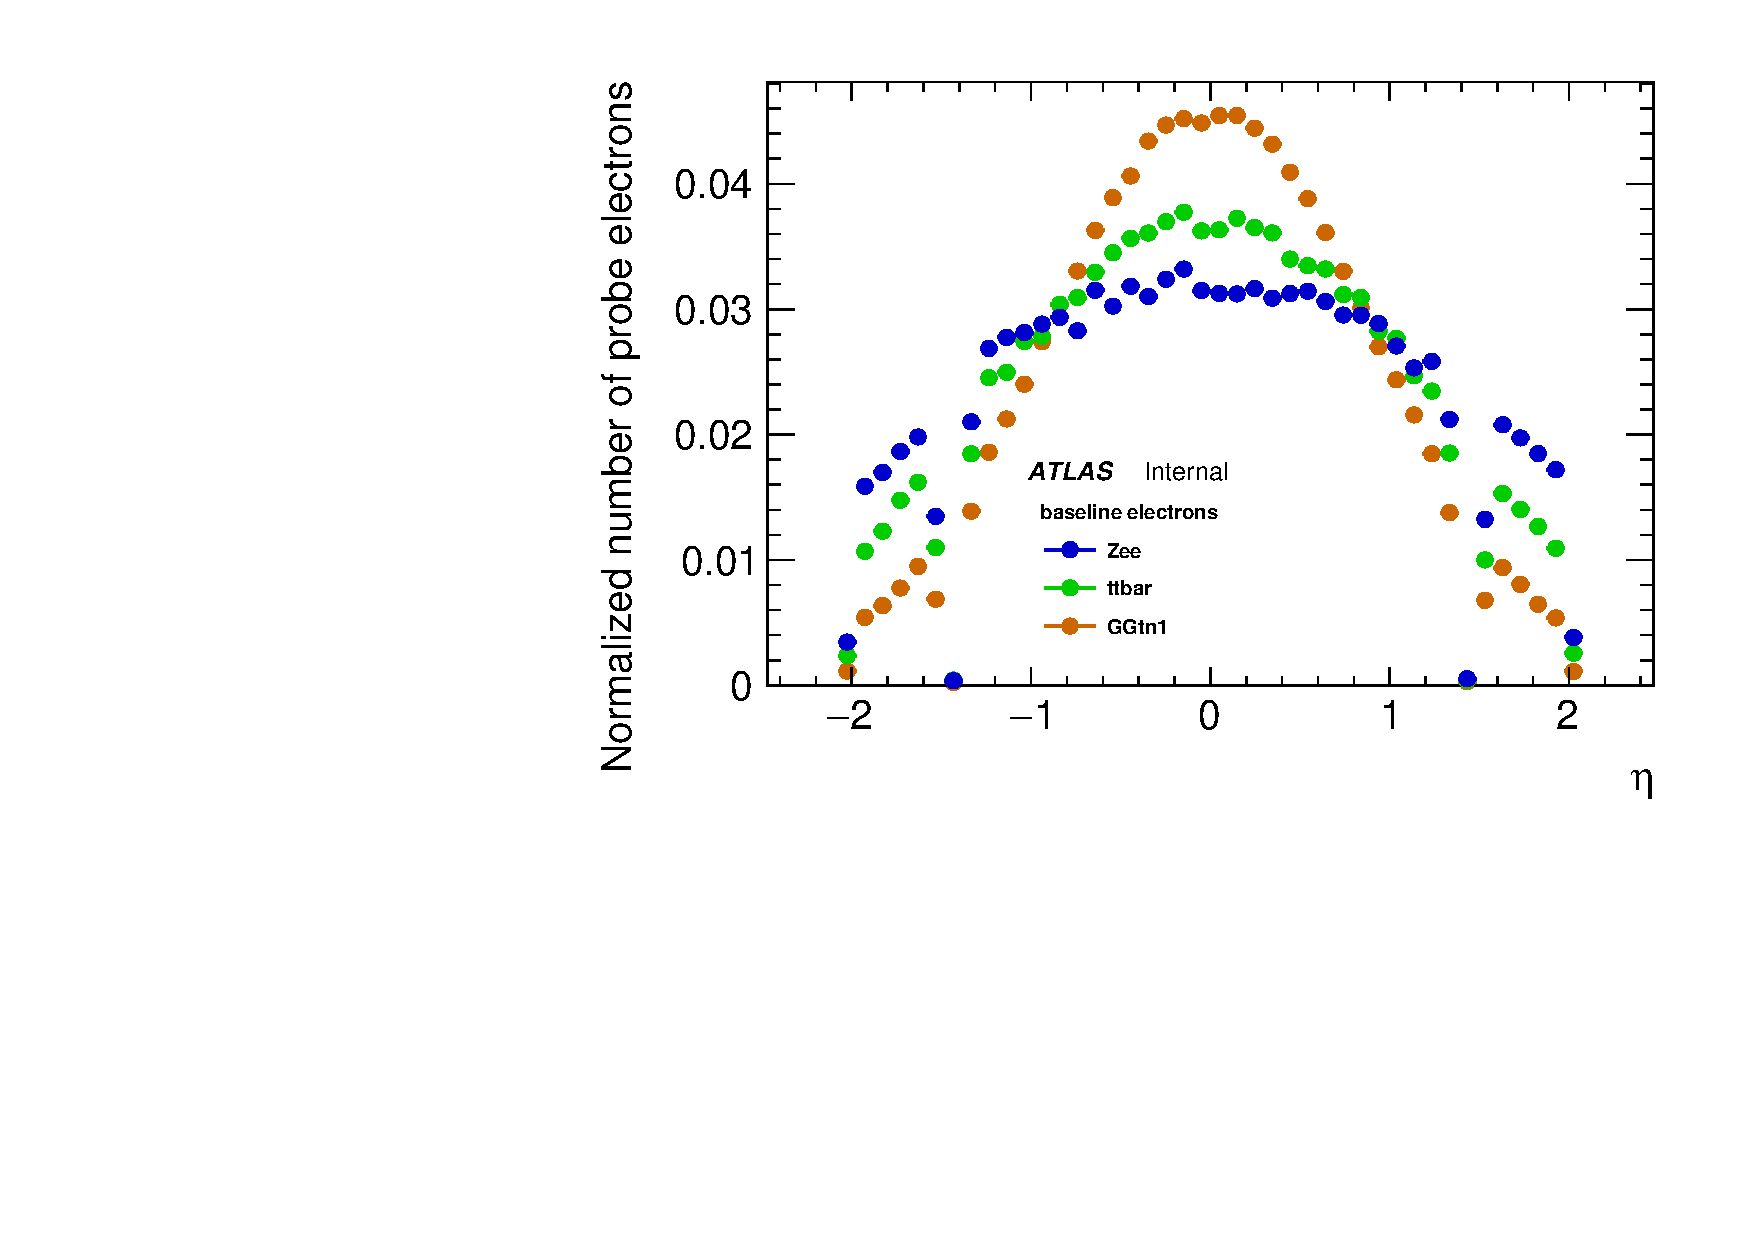
\includegraphics[width=0.4\textwidth]{BKG/realEff/Syst/Syst_Topo_baseline_eta_distribution_electrons.pdf} 
	   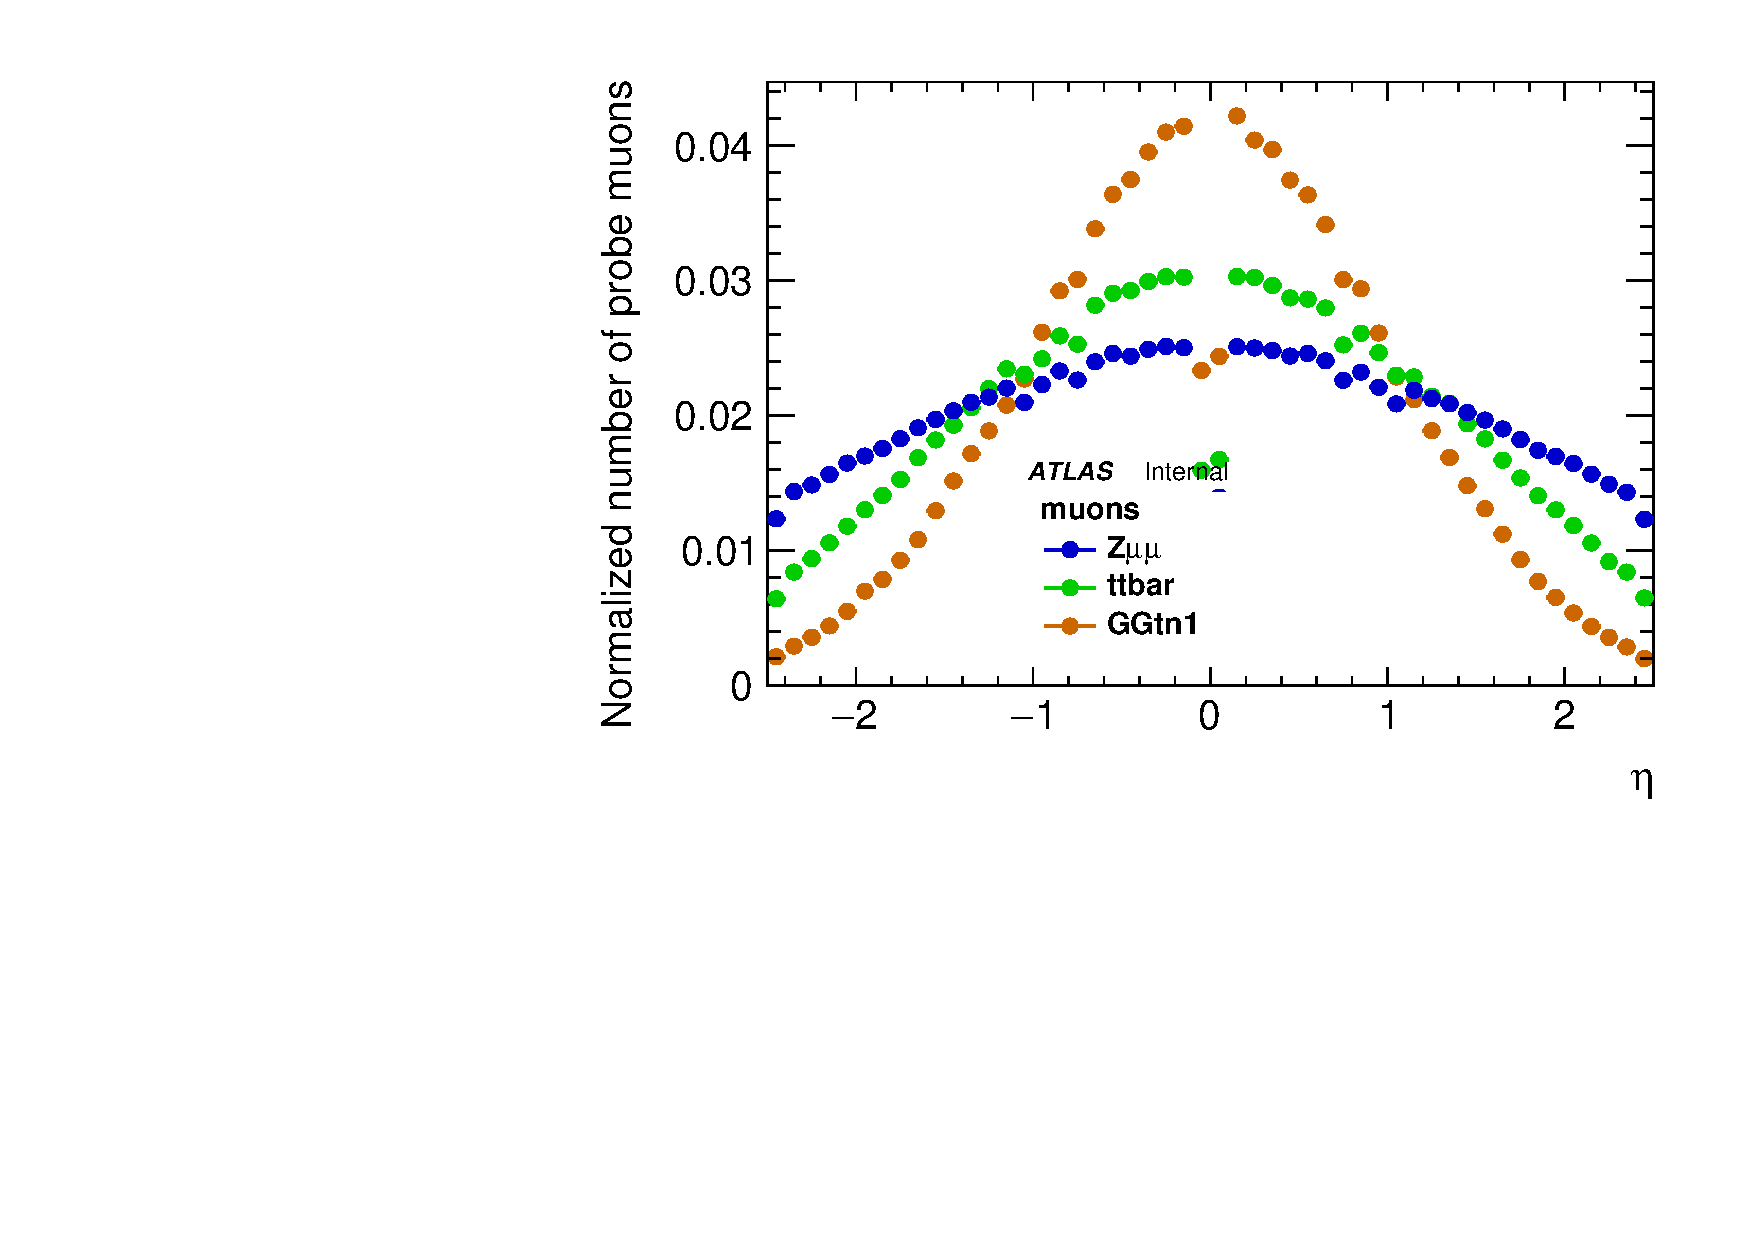
\includegraphics[width=0.4\textwidth]{BKG/realEff/Syst/Syst_Topo_baseline_eta_distribution_muons.pdf}
	   \caption{\label{fig:Syst_kinematics} $\pt$ (top) and $\eta$ baseline electron (left) and muons (right) distributions. Three processes are considered, $Z\rightarrow ll$ (blue), $t\overline{t}$ (green) and  $\tilde{g}\tilde{g} \rightarrow t\overline{t}t\overline{t} \tilde{\chi}^0_1 \tilde{\chi}^0_1$ with $m_{\tilde{g}} - m_{\tilde{\chi}^0_1} > 1000$ GeV (orange). A truth match on the leptons is applied.}
	  \end{center}
	\end{figure}	
%%%%%%%%%%%%%%%%%%%%%%%%%%%%%%%%%%%%%%%%%%%%%%%%%%%%%%%%%%%%	

	
	Figure \ref{fig:Syst_topo} shows the $\Delta R(\ell,\mathrm{jet})$ (top) and $n_{\mathrm{Jets}}$ (bottom) distribution of truth matched baseline lepton extracted from $Z \rightarrow ll$, $t\overline{t}$ and the SUSY benchmark processes. The $\Delta R(\ell,\mathrm{jet})$ distribution associated to the SUSY signals peaks at 0.3 and most of the statistics is contained in the $\Delta R(\ell,\mathrm{jet}) < 1$ range. In comparison $\sim 60\%$ of the electrons from $Z \rightarrow ll$, $t\overline{t}$ are not accompanied with a signal jet and the $\Delta R(\ell,\mathrm{jet})$ distribution of remaining leptons peaks at $\pi$. The jet multiplicity of the $Z\rightarrow ll$ electrons peaks at 0 jets whereas the benchmark SUSY signal ones at 8 jets. These plots confirm that the leptons produced in the SUSY benchmarks are accompanied with much more jets and are therefore less isolated than the ones form $Z\rightarrow \ell\ell$ processes. Considering this extreme topology enables to assess a conservative SUSY signal topology extrapolation systematic that should cover all SUSY signal processes considered by the analysis.
	
	
%%%%%%%%%%%%%%%%%%%%%%%%%%%%%%%%%%%%%%%%%%%%%%%%%%%%%%%%%%%	
\begin{figure}[!h]
	\begin{center} 
	   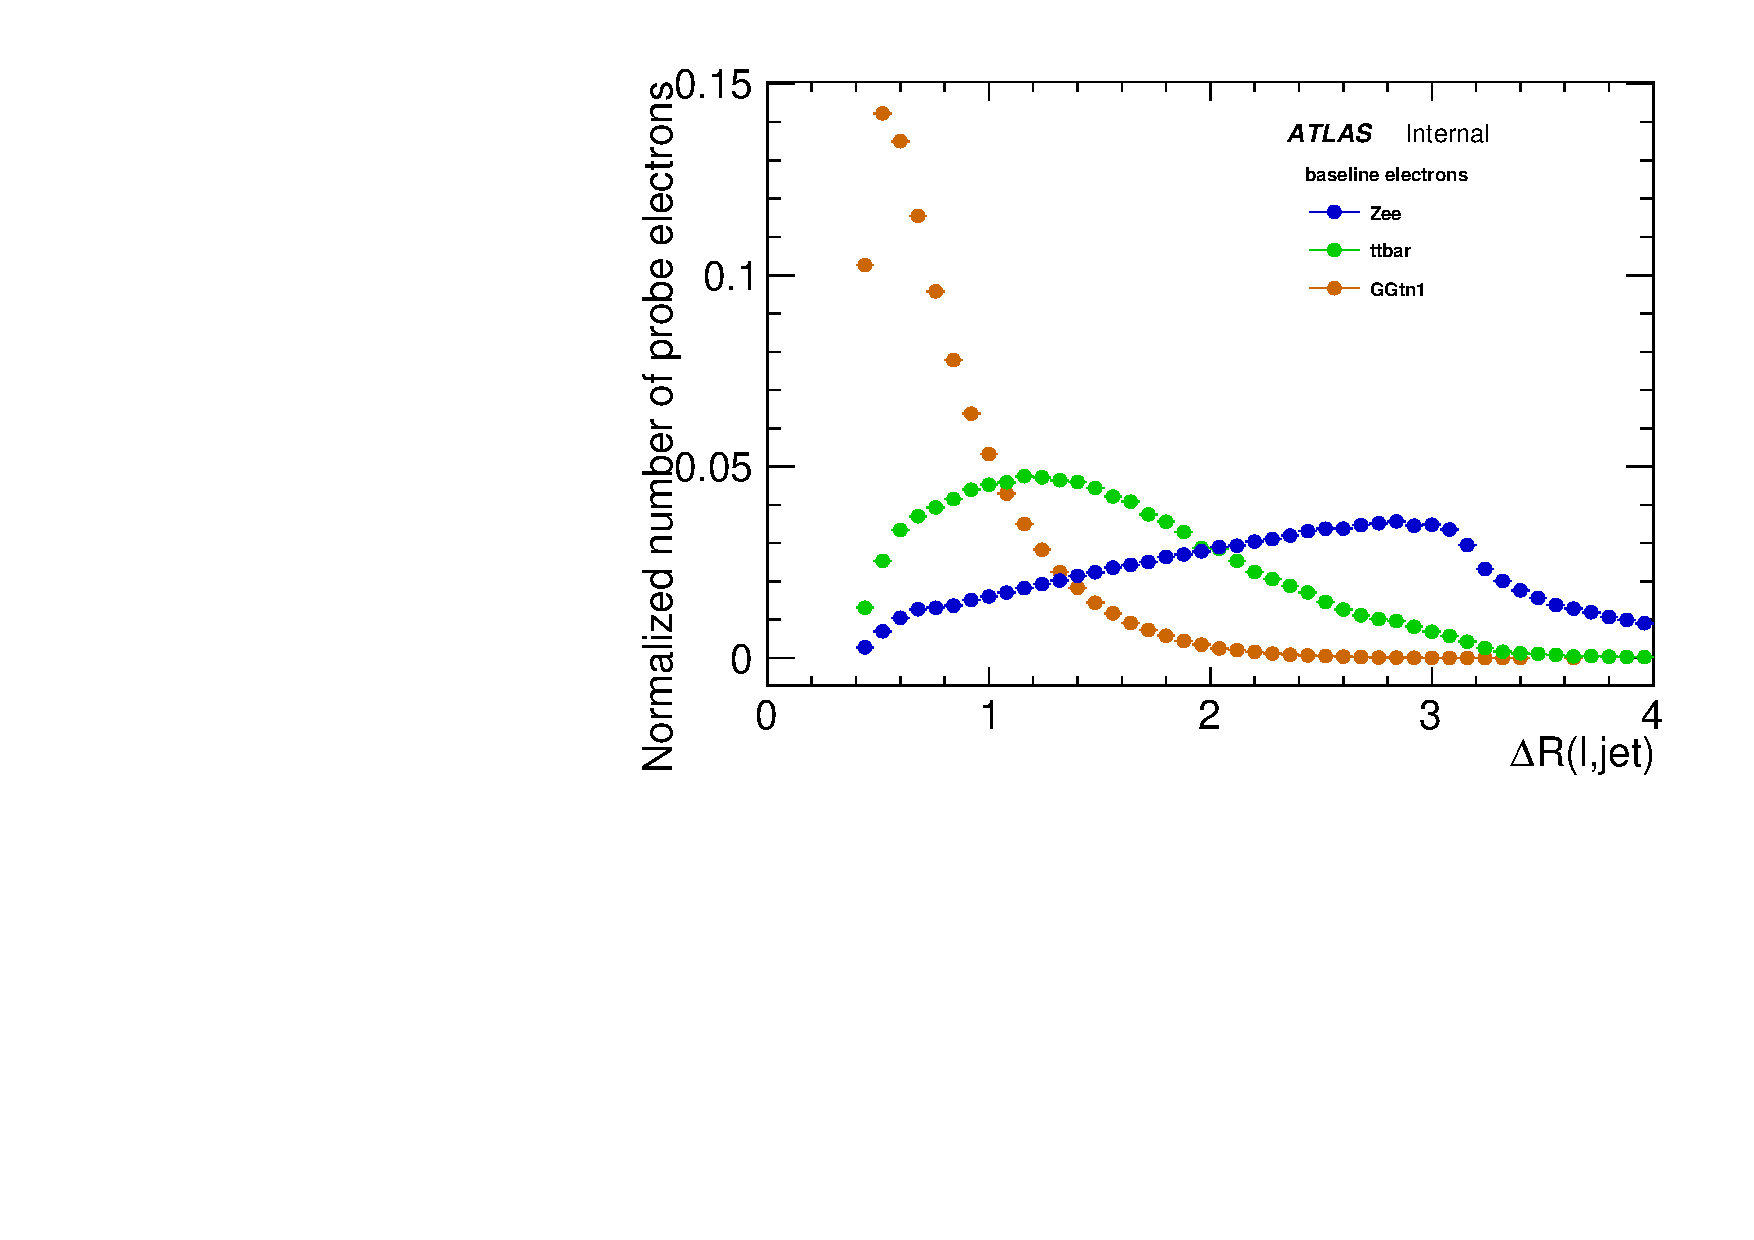
\includegraphics[width=0.4\textwidth]{BKG/realEff/Syst/Syst_Topo_baseline_DRjet_distribution_electrons.pdf} 
	   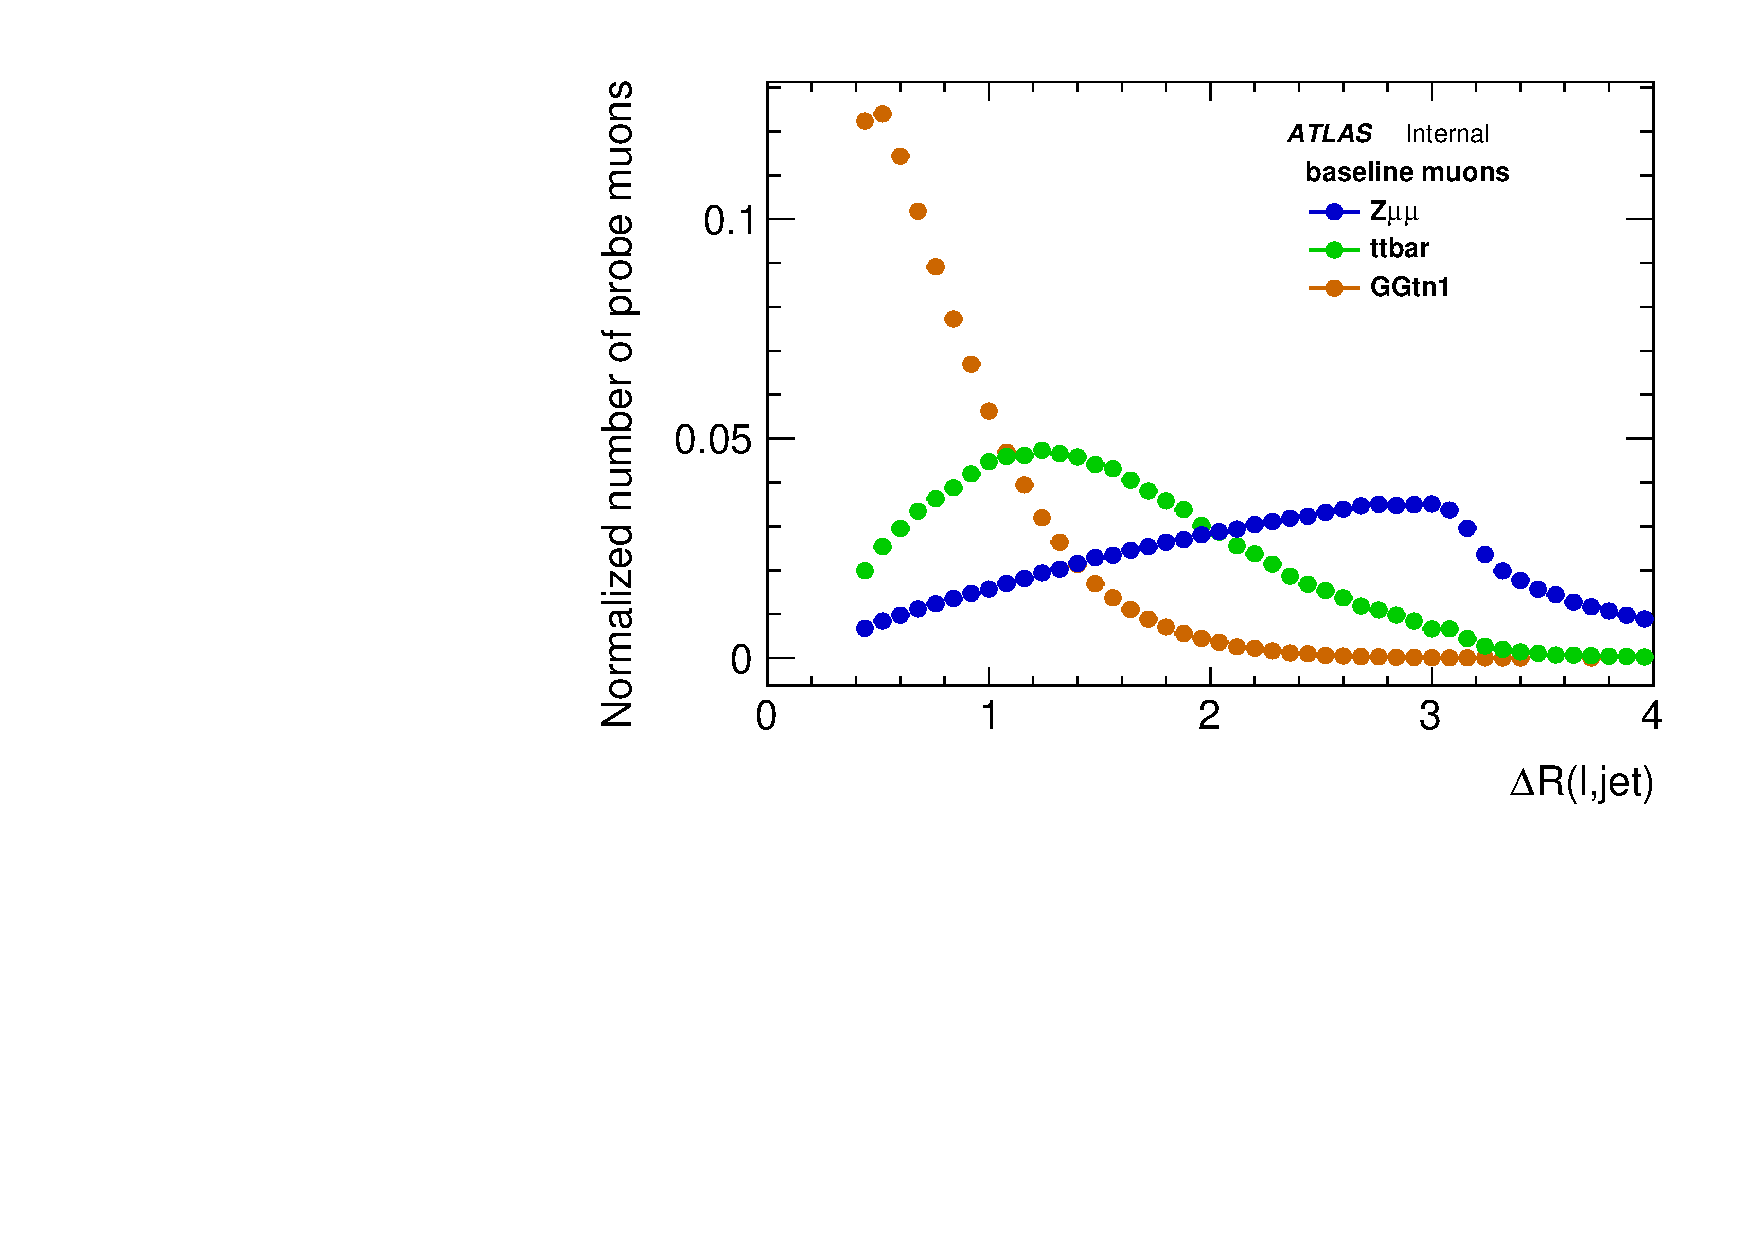
\includegraphics[width=0.4\textwidth]{BKG/realEff/Syst/Syst_Topo_baseline_DRjet_distribution_muons.pdf}
	   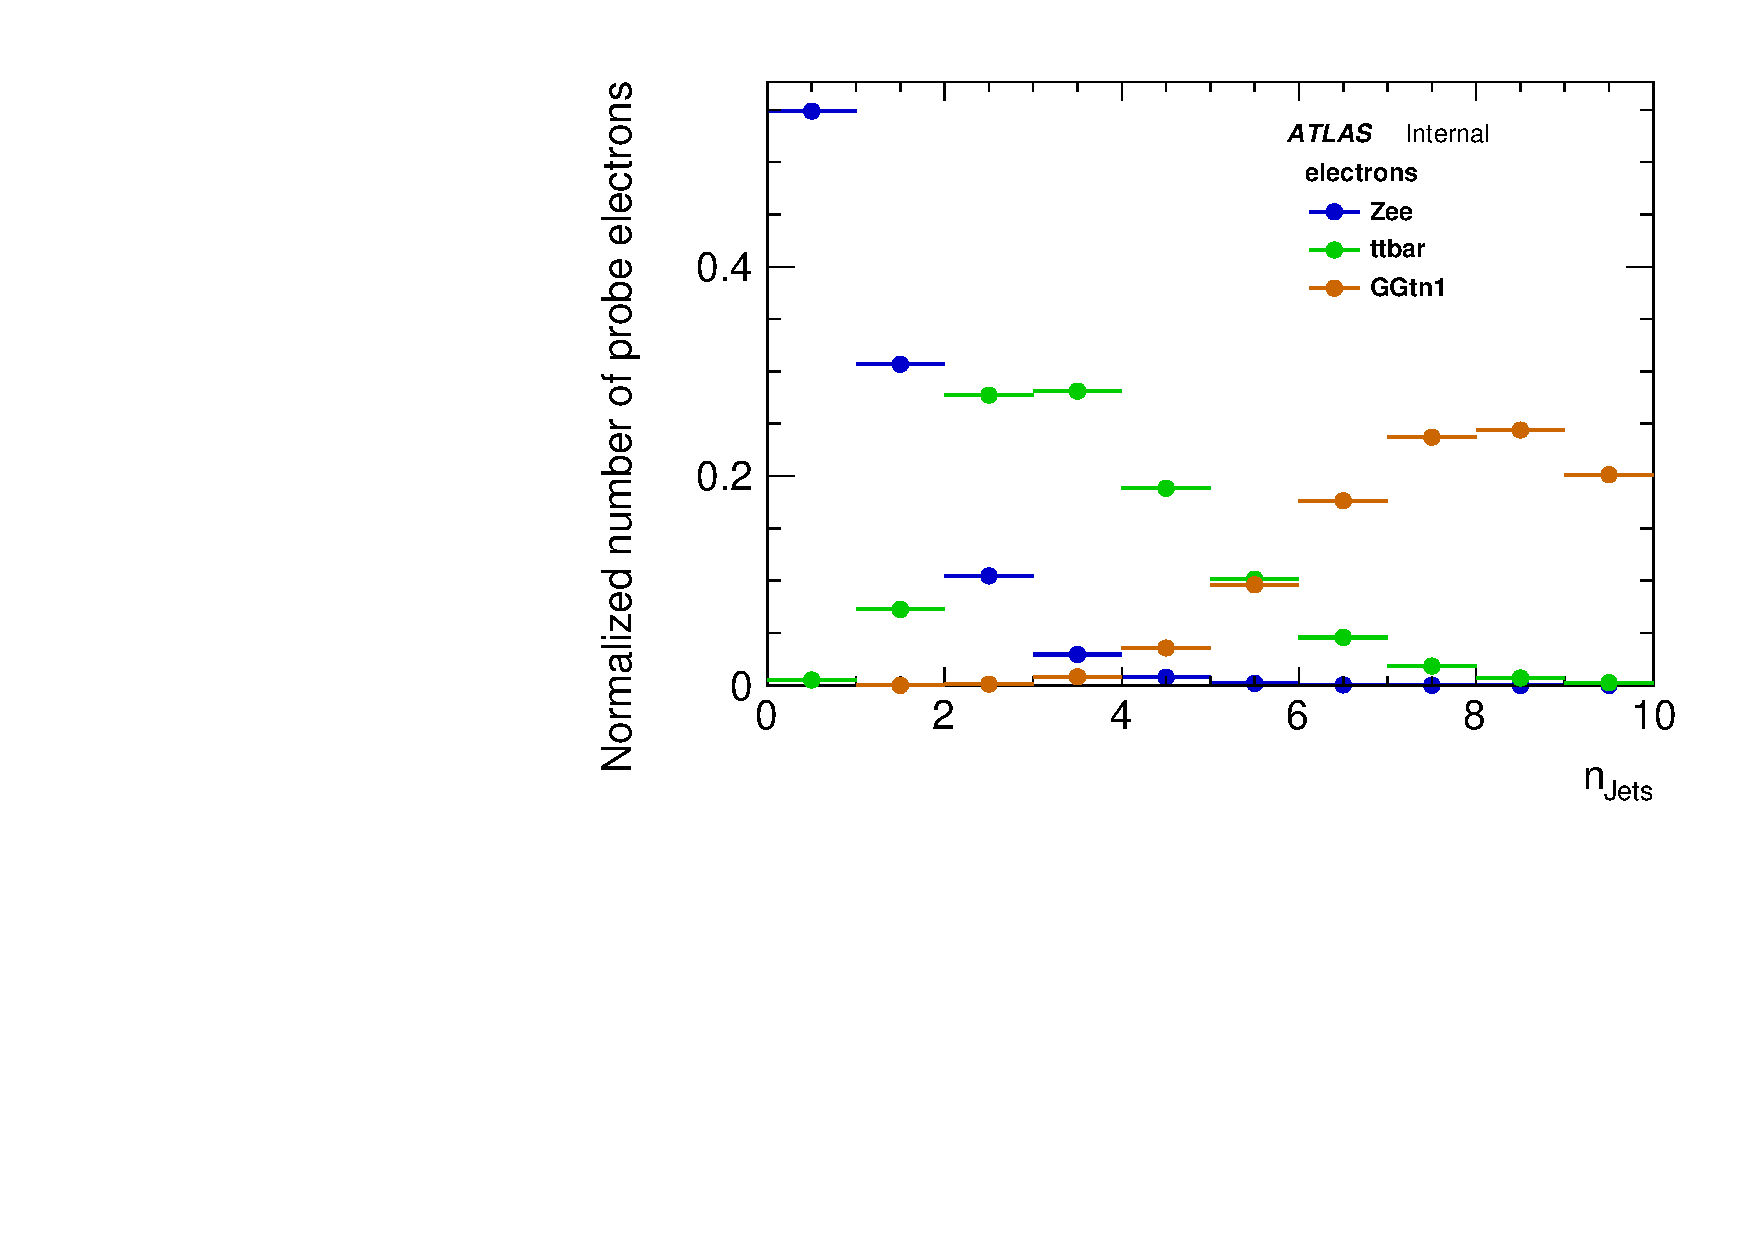
\includegraphics[width=0.4\textwidth]{BKG/realEff/Syst/Syst_Topo_baseline_nJets_distribution_electrons.pdf} 
	   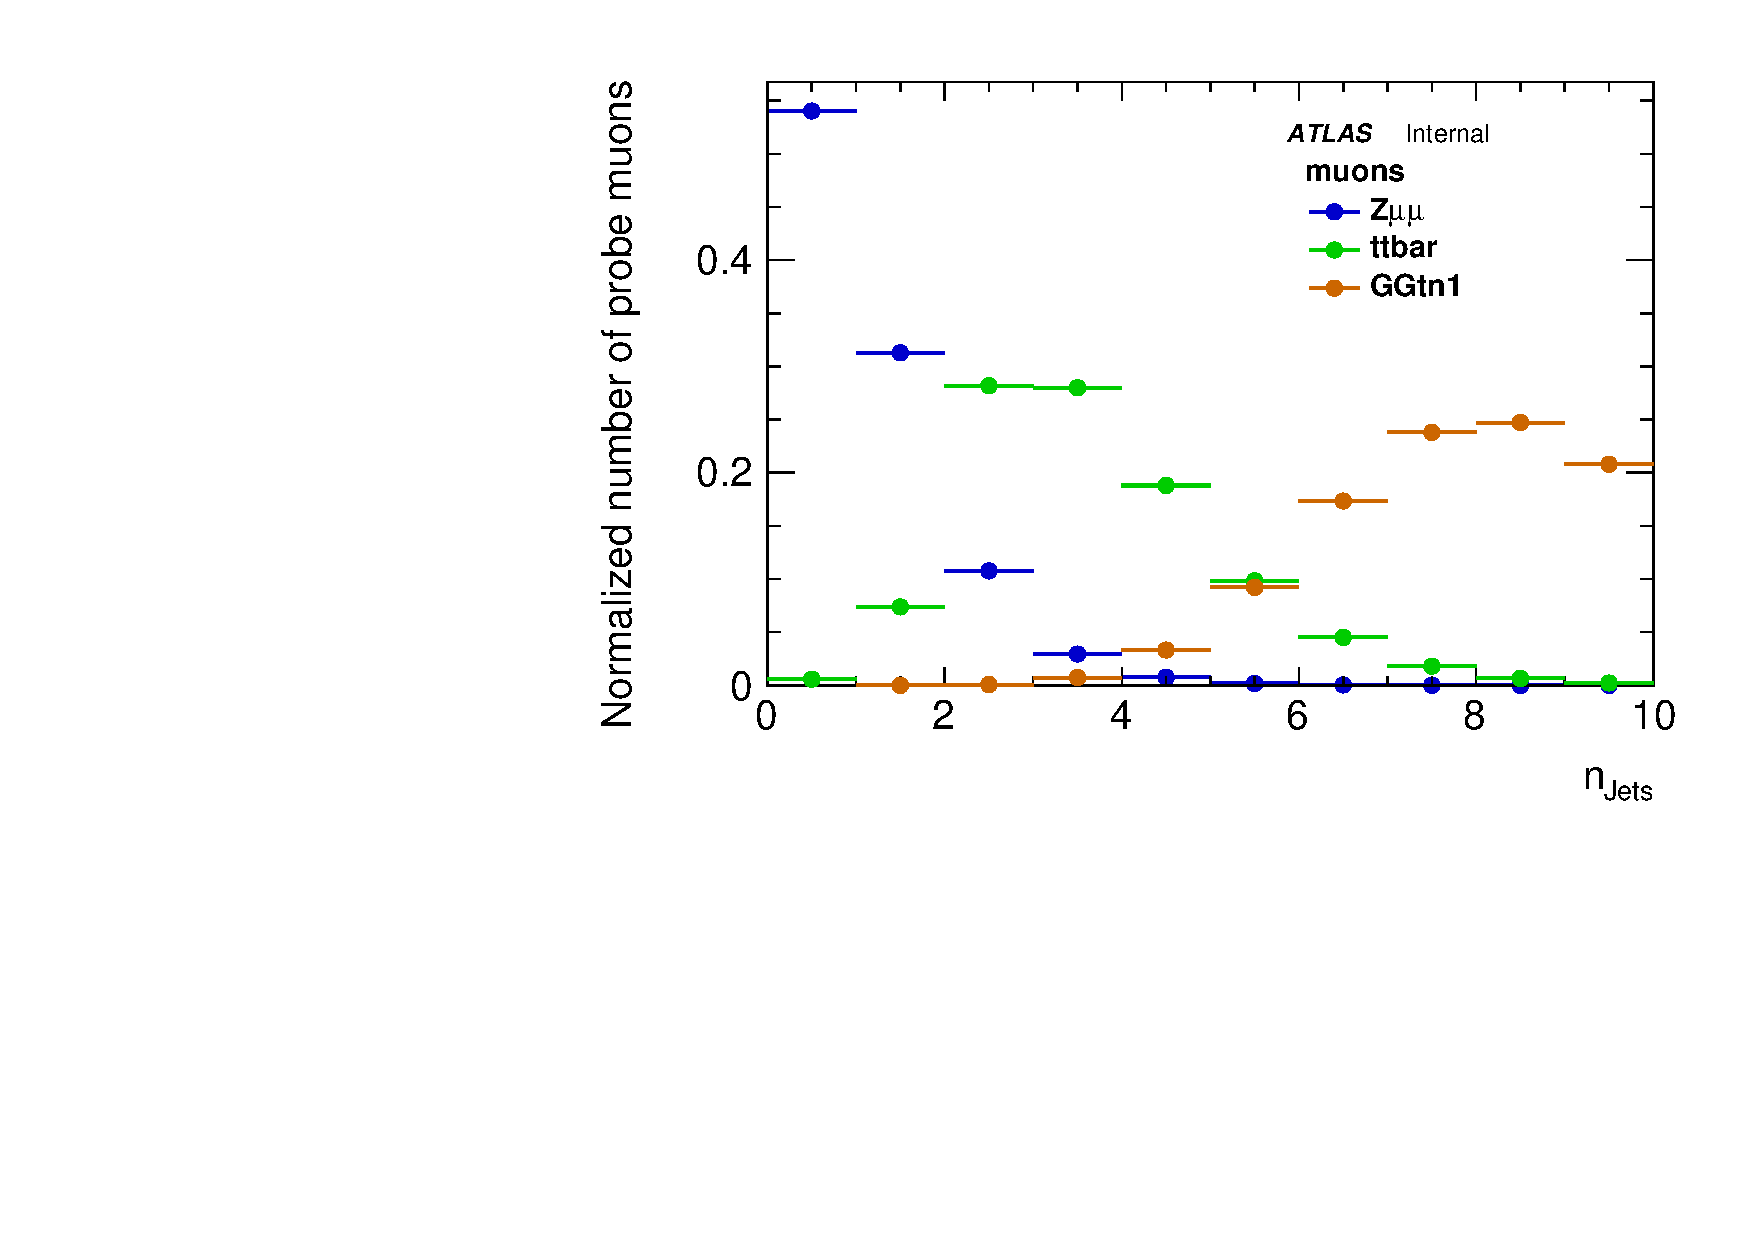
\includegraphics[width=0.4\textwidth]{BKG/realEff/Syst/Syst_Topo_baseline_nJets_distribution_muons.pdf}
	   \caption{\label{fig:Syst_topo} $\Delta R(\ell,\mathrm{jet})$ (top) and $n_{Jets}$ (bottom) baseline electron (left) and muons (right) distributions. Three processes are considered, $Z\rightarrow ll$ (blue), $t\overline{t}$ (green) and  $\tilde{g}\tilde{g} \rightarrow t\overline{t}t\overline{t} \tilde{\chi}^0_1 \tilde{\chi}^0_1$ with $m_{\tilde{g}} - m_{\tilde{\chi}^0_1} > 1000$ GeV (orange). A truth match on the leptons is applied.}
	\end{center}
\end{figure}	
%%%%%%%%%%%%%%%%%%%%%%%%%%%%%%%%%%%%%%%%%%%%%%%%%%%%%%%%%%%%	


	Figure \ref{fig:Syst_Eff_Vs_pt} shows the real lepton efficiencies as a function of $\pt$. These efficiencies are computed with truth matched lepton from $Z \rightarrow ll$, $t\overline{t}$ and $\tilde{g}\tilde{g} \rightarrow t\overline{t}t\overline{t} \tilde{\chi}^0_1 \tilde{\chi}^0_1$. The $Z \rightarrow ll$ and $t\overline{t}$ leptons are reweighed to the signal \pt distributions as large difference were found in the \pt distributions. The ratio shown in the efficiencies plots corresponds to the $\tilde{g}\tilde{g} \rightarrow t\overline{t}t\overline{t} \tilde{\chi}^0_1 \tilde{\chi}^0_1$ efficiencies divided the $Z \rightarrow ll$ ones. 
	The left plot, dedicated to the electron efficiencies as a function of $\pt$, shows that the $Z\rightarrow ll$ to SUSY signal efficiency ratio is $\pt$ dependent in the $\pt < 40$ GeV range and stabilize in the $\pt > 40$ GeV range. The observed differences are mostly due to the calorimeter isolation cut and the track isolation in a lesser extent at low \pt. The right plot dedicated to muons efficiencies shows that the $\pt$ dependency of ratio is more pronounced in the muon case because of the $d_{0}/\sigma_{d_{0}}$ cut (which induces \pt dependent differences). The associated relative efficiencies differences starts with $13\%$ at low $\pt$ and decrease down to $\sim 1\%$ in the $\pt > 80$ GeV range. In a lesser extent, the track isolation cut also induces efficiency differences at low \pt. \\ 
	

%%%%%%%%%%%%%%%%%%%%%%%%%%%%%%%%%%%%%%%%%%%%%%%%%%%%%%%%%%%%	
\begin{figure}[!h]
	\begin{center} 
	   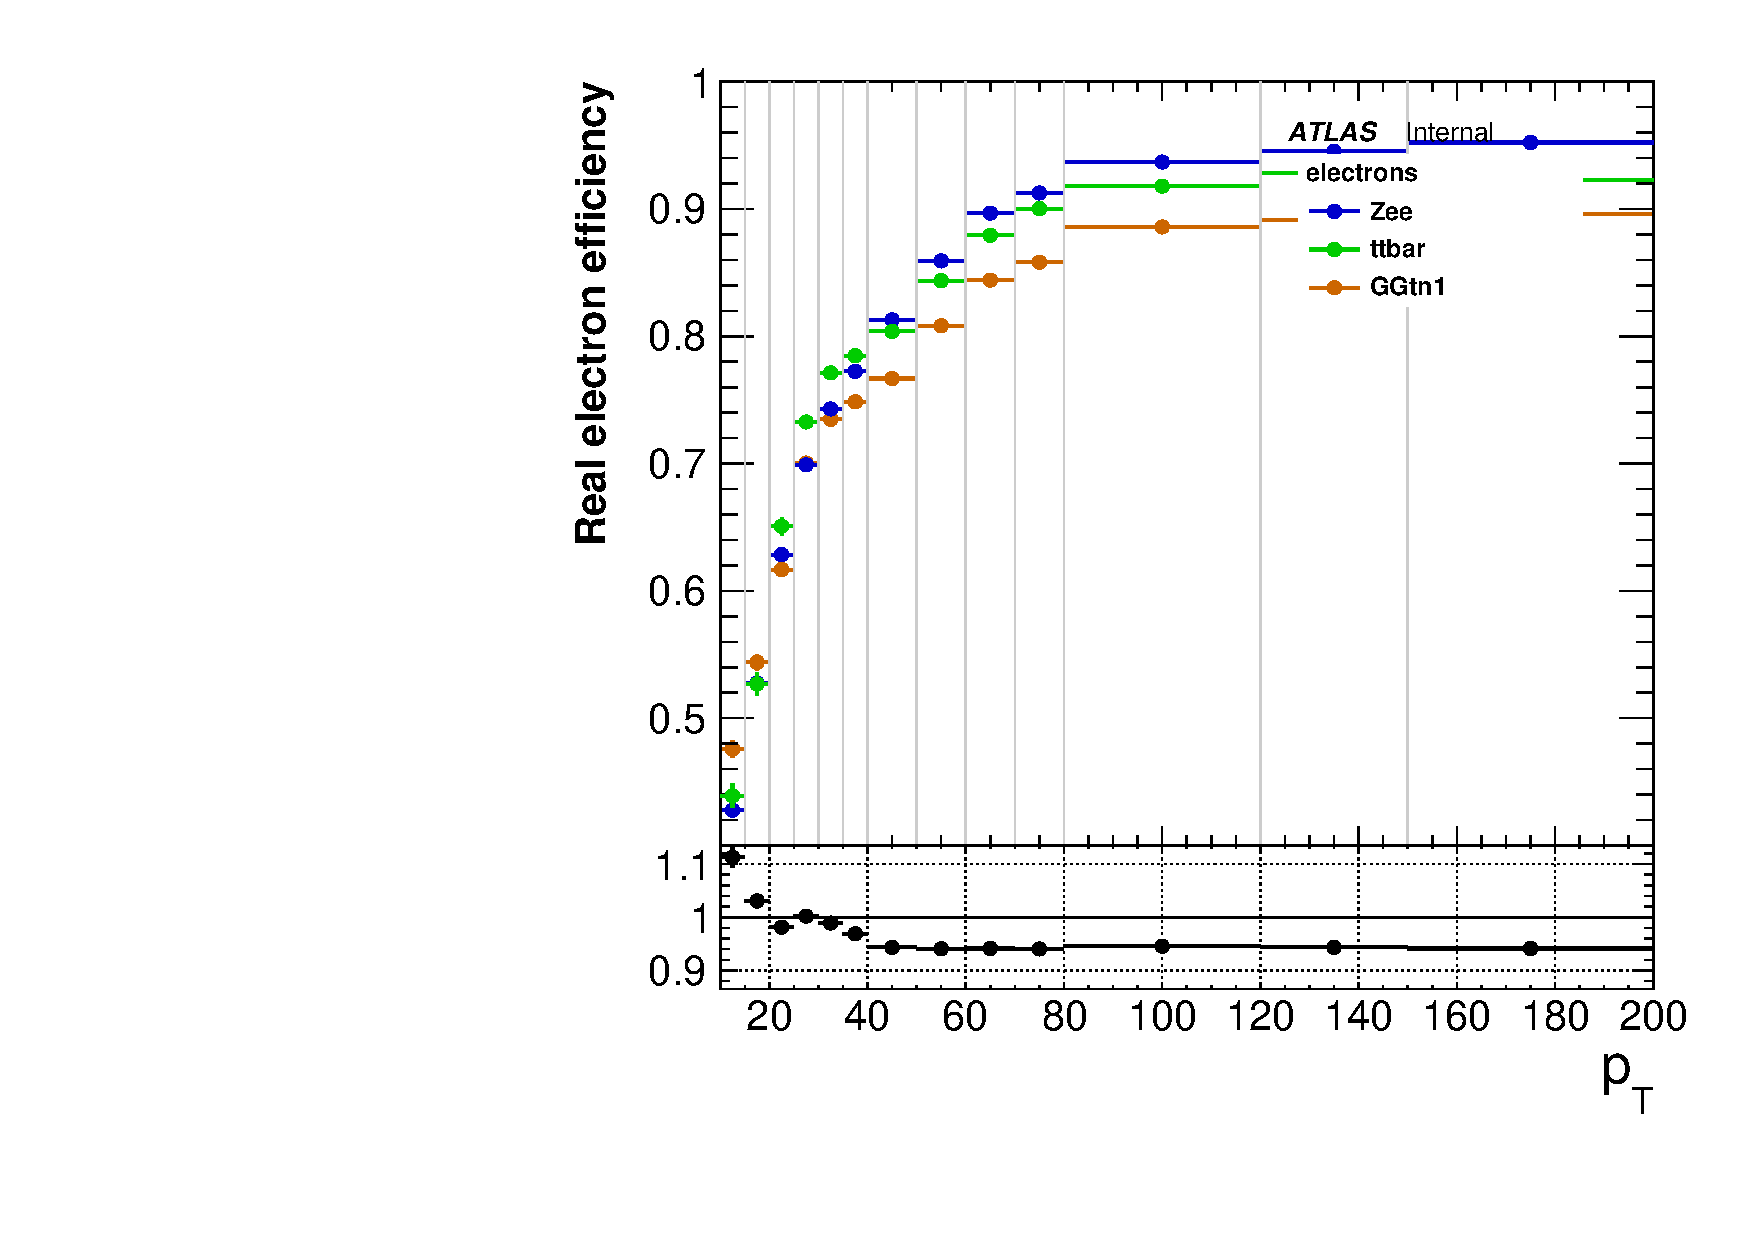
\includegraphics[width=0.4\textwidth]{BKG/realEff/Syst/Syst_Topo_RealEfficiencies_Vs_pt_electrons.pdf} 
	   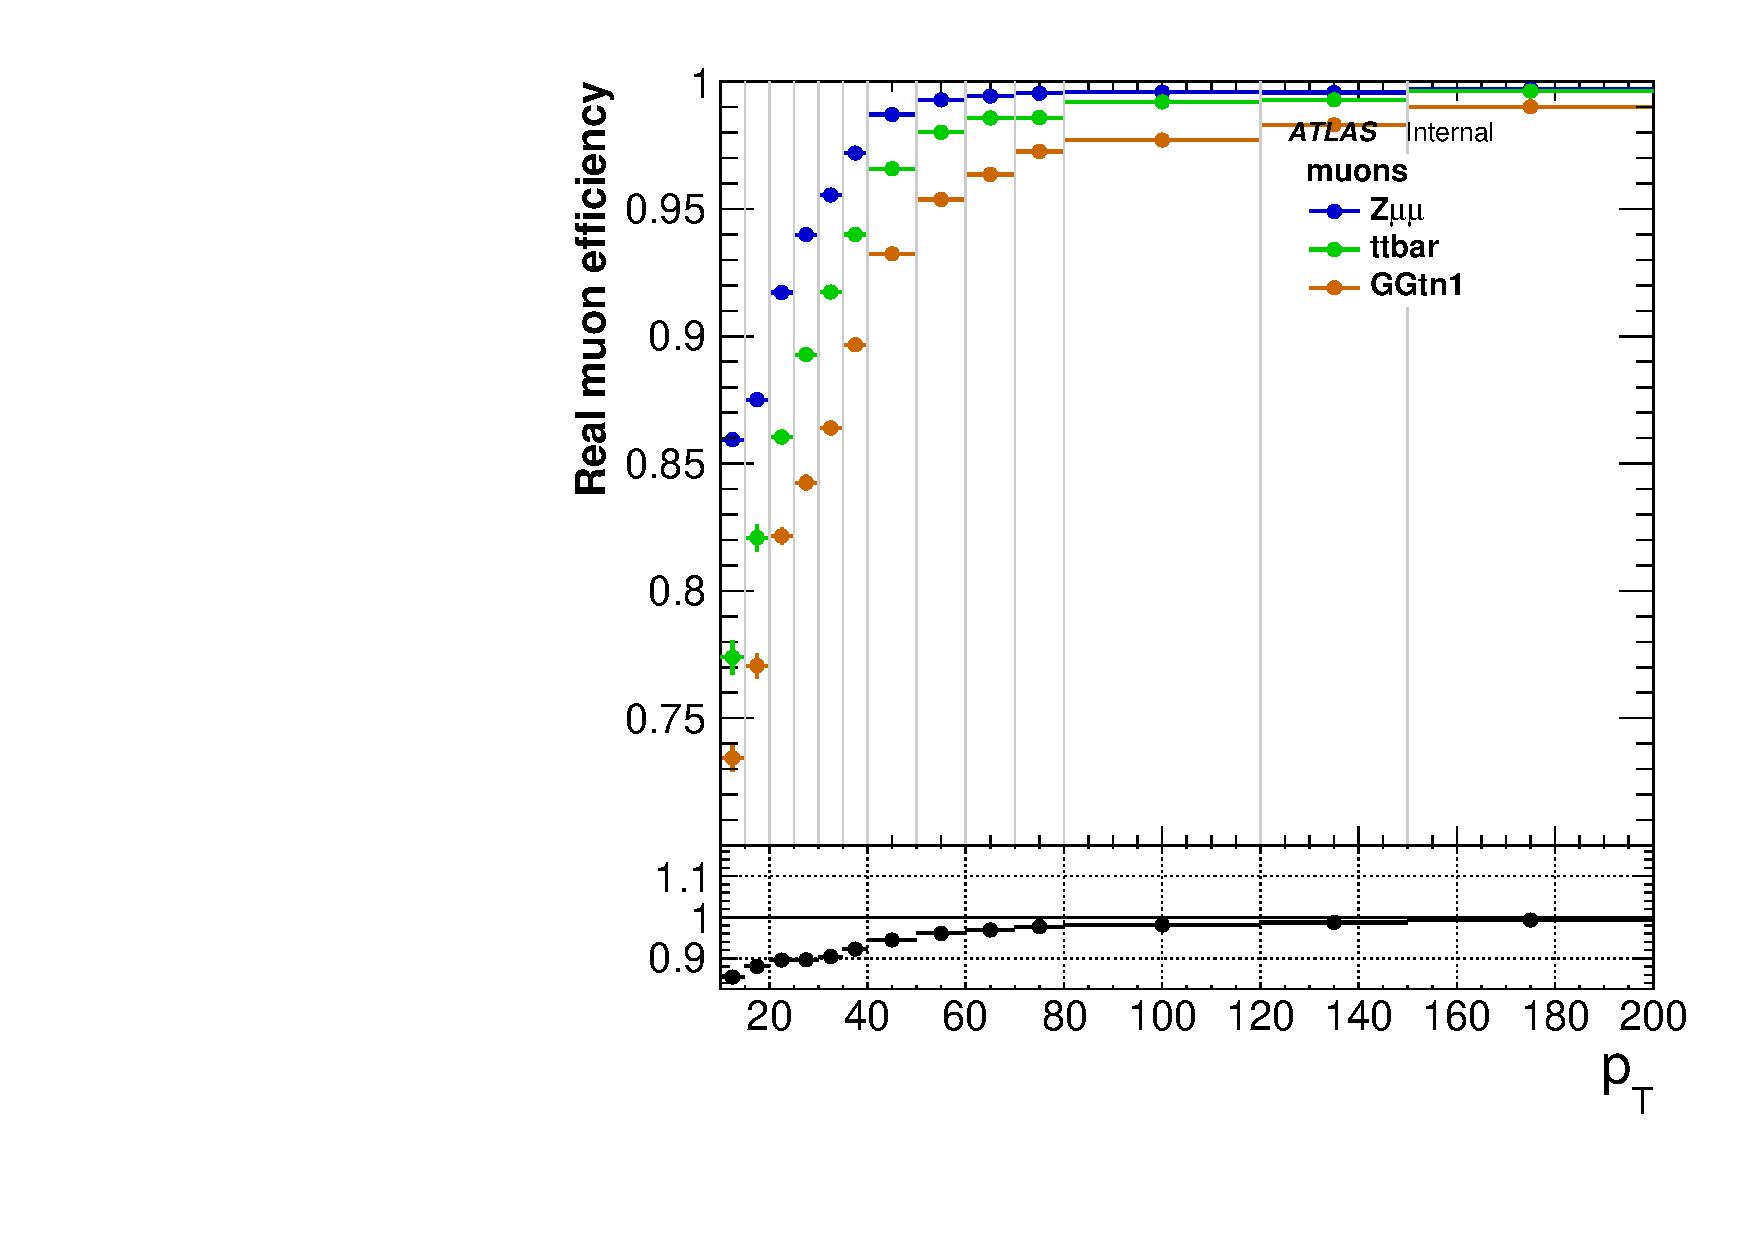
\includegraphics[width=0.4\textwidth]{BKG/realEff/Syst/Syst_Topo_RealEfficiencies_Vs_pt_muons.pdf}
	   \caption{\label{fig:Syst_Eff_Vs_pt} Real electron (left) and muon (right) efficiencies as a function $\pt$. Three processes are considered, $Z\rightarrow ll$ (blue), $t\overline{t}$ (green) and  $\tilde{g}\tilde{g} \rightarrow t\overline{t}t\overline{t} \tilde{\chi}^0_1 \tilde{\chi}^0_1$ with $m_{\tilde{g}} - m_{\tilde{\chi}^0_1} > 1000$ GeV (orange). A truth match on the leptons is applied and a $\pt$ reweighing to the SUSY signal electron $\pt$ is used to compute the efficiencies.}
	\end{center}
\end{figure}	
%%%%%%%%%%%%%%%%%%%%%%%%%%%%%%%%%%%%%%%%%%%%%%%%%%%%%%%%%%%		


	As tight isolation cuts are use to define signal electrons, the very different (b-)jet multiplicity of the process is expected to induce $\Delta R(\ell,\mathrm{jet})$ dependent efficiencies differences. Figure \ref{fig:Syst_Eff_Vs_DRjet} shows the real electron (top) and muon (bottom) efficiencies as a function of $\Delta R(l,jets)$ considering three characteristic \pt ranges : [15-20], [40-50] and [70-80] GeV. As expected a large SUSY signal efficiency decrease is observed in the $\Delta R(\ell,\mathrm{jet})[0.4-0.6]$ range for all the \pt range and for both electrons and muons. The efficiency losses are smaller for $Z\rightarrow \ell\ell$ events in almost all the configurations, therefore larger efficiencies differences are observed at low $\Delta R(\ell,\mathrm{jet})$ range. Nevertheless, for electrons with $\pt > 60$ GeV, the ratio between $Z$ and $\tilde{g}\tilde{g} \rightarrow t\overline{t}t\overline{t} \tilde{\chi}^0_1 \tilde{\chi}^0_1$ efficiencies are flat as a function of $\Delta R(\ell,\mathrm{jet})$. As already observed in Figure \ref{fig:Syst_Eff_Vs_pt} the $Z$ to signal muon efficiencies differences decreases as a function of \pt.


%%%%%%%%%%%%%%%%%%%%%%%%%%%%%%%%%%%%%%%%%%%%%%%%%%%%%%%%%%%%	
\begin{figure}[!h]
	\begin{center} 
	   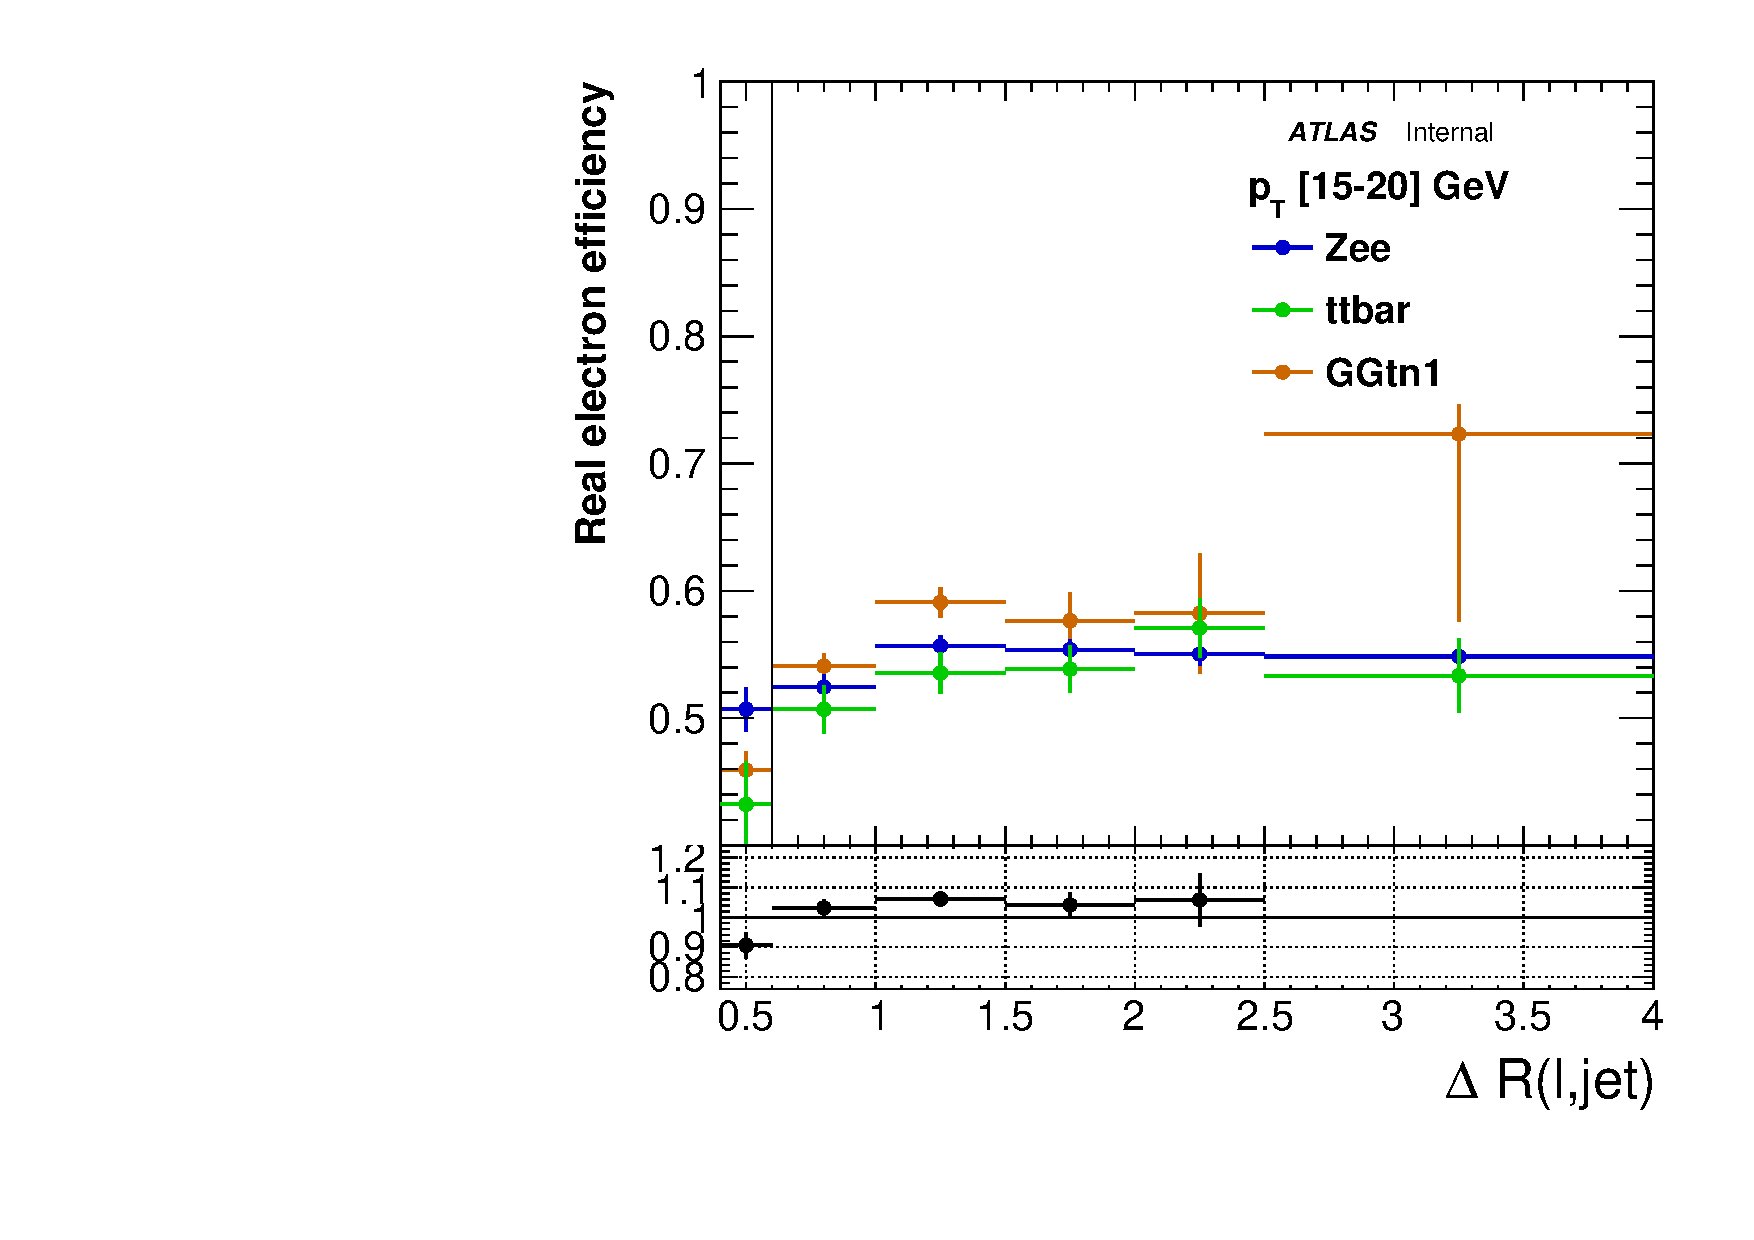
\includegraphics[width=0.3\textwidth]{BKG/realEff/Syst/Syst_Topo_RealEfficiencies_Vs_DRjet_electronspt_range_15_20.pdf} 
	   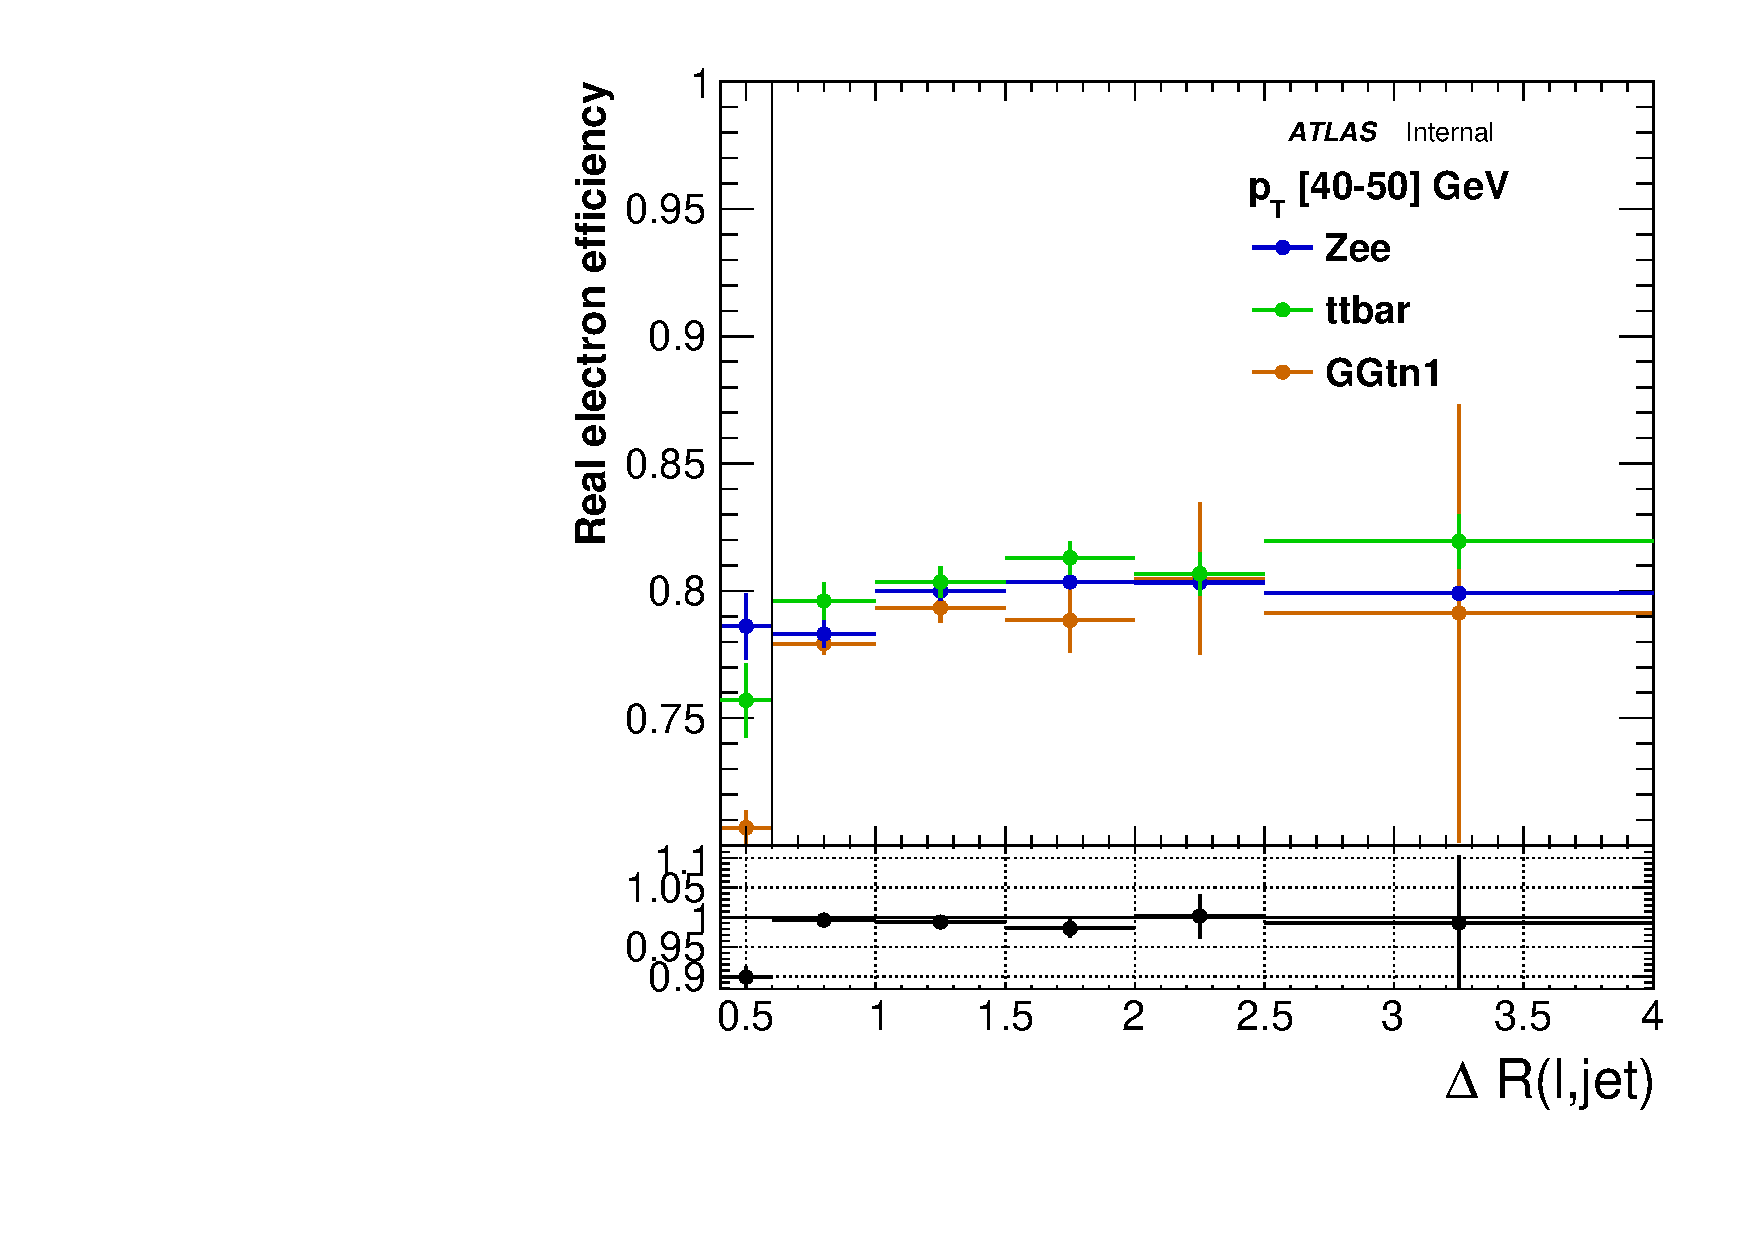
\includegraphics[width=0.3\textwidth]{BKG/realEff/Syst/Syst_Topo_RealEfficiencies_Vs_DRjet_electronspt_range_40_50.pdf} 
	   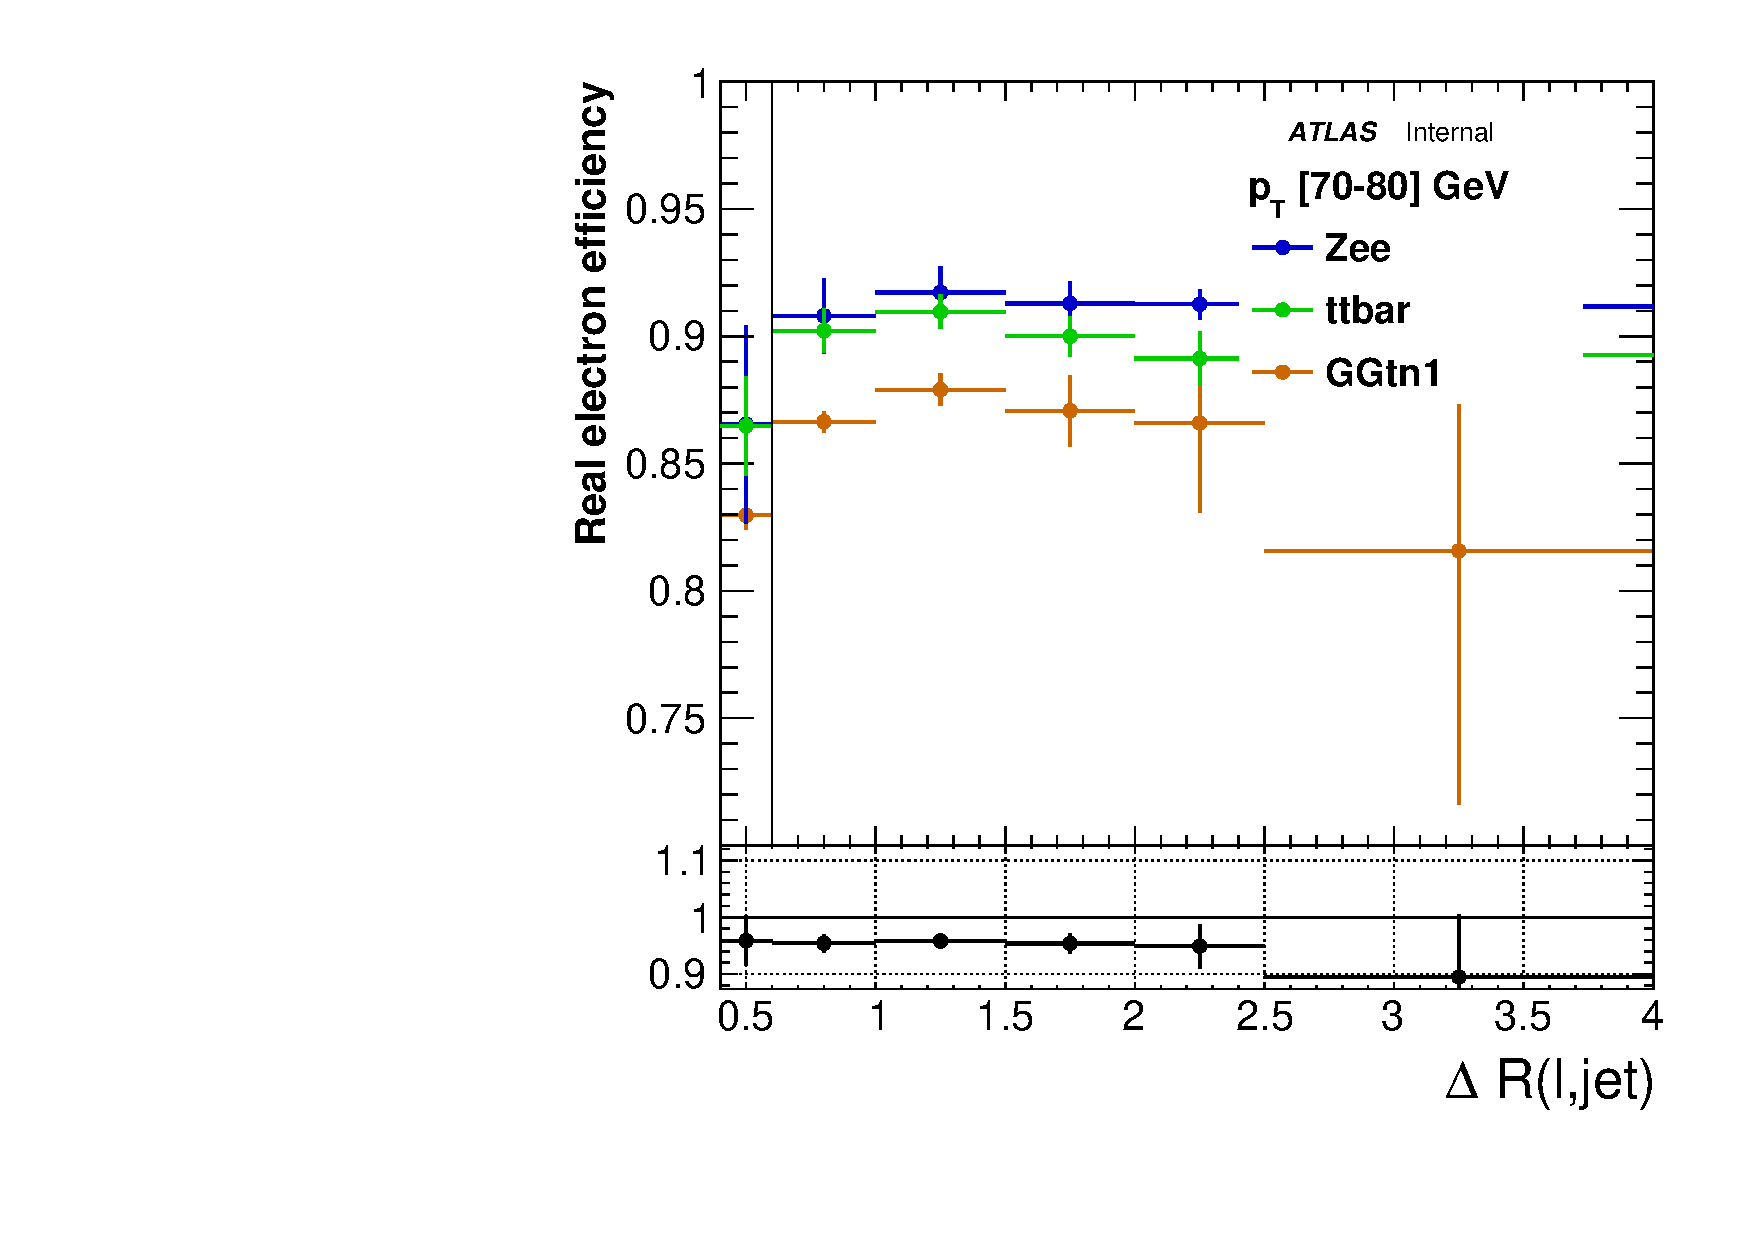
\includegraphics[width=0.3\textwidth]{BKG/realEff/Syst/Syst_Topo_RealEfficiencies_Vs_DRjet_electronspt_range_70_80.pdf}
	   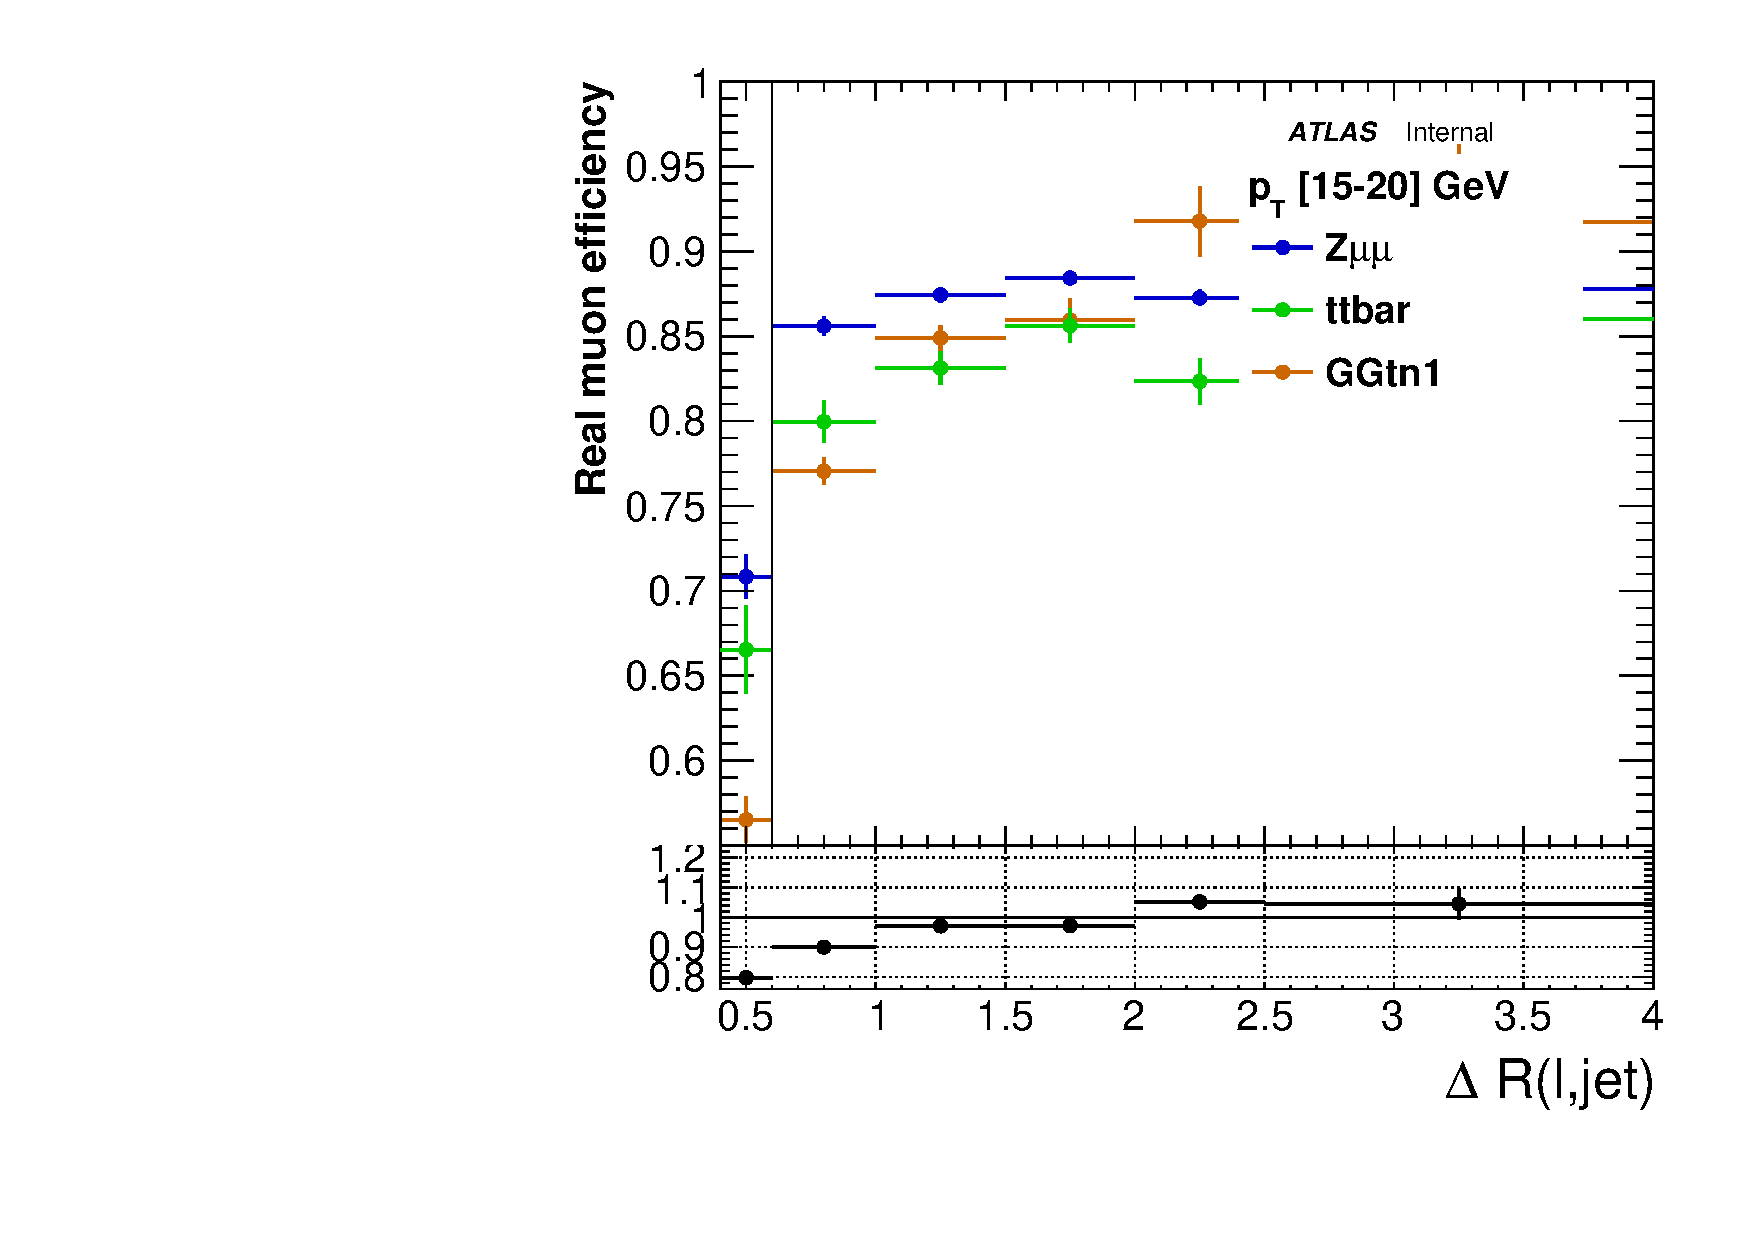
\includegraphics[width=0.3\textwidth]{BKG/realEff/Syst/Syst_Topo_RealEfficiencies_Vs_DRjet_muonspt_range_15_20.pdf}
	   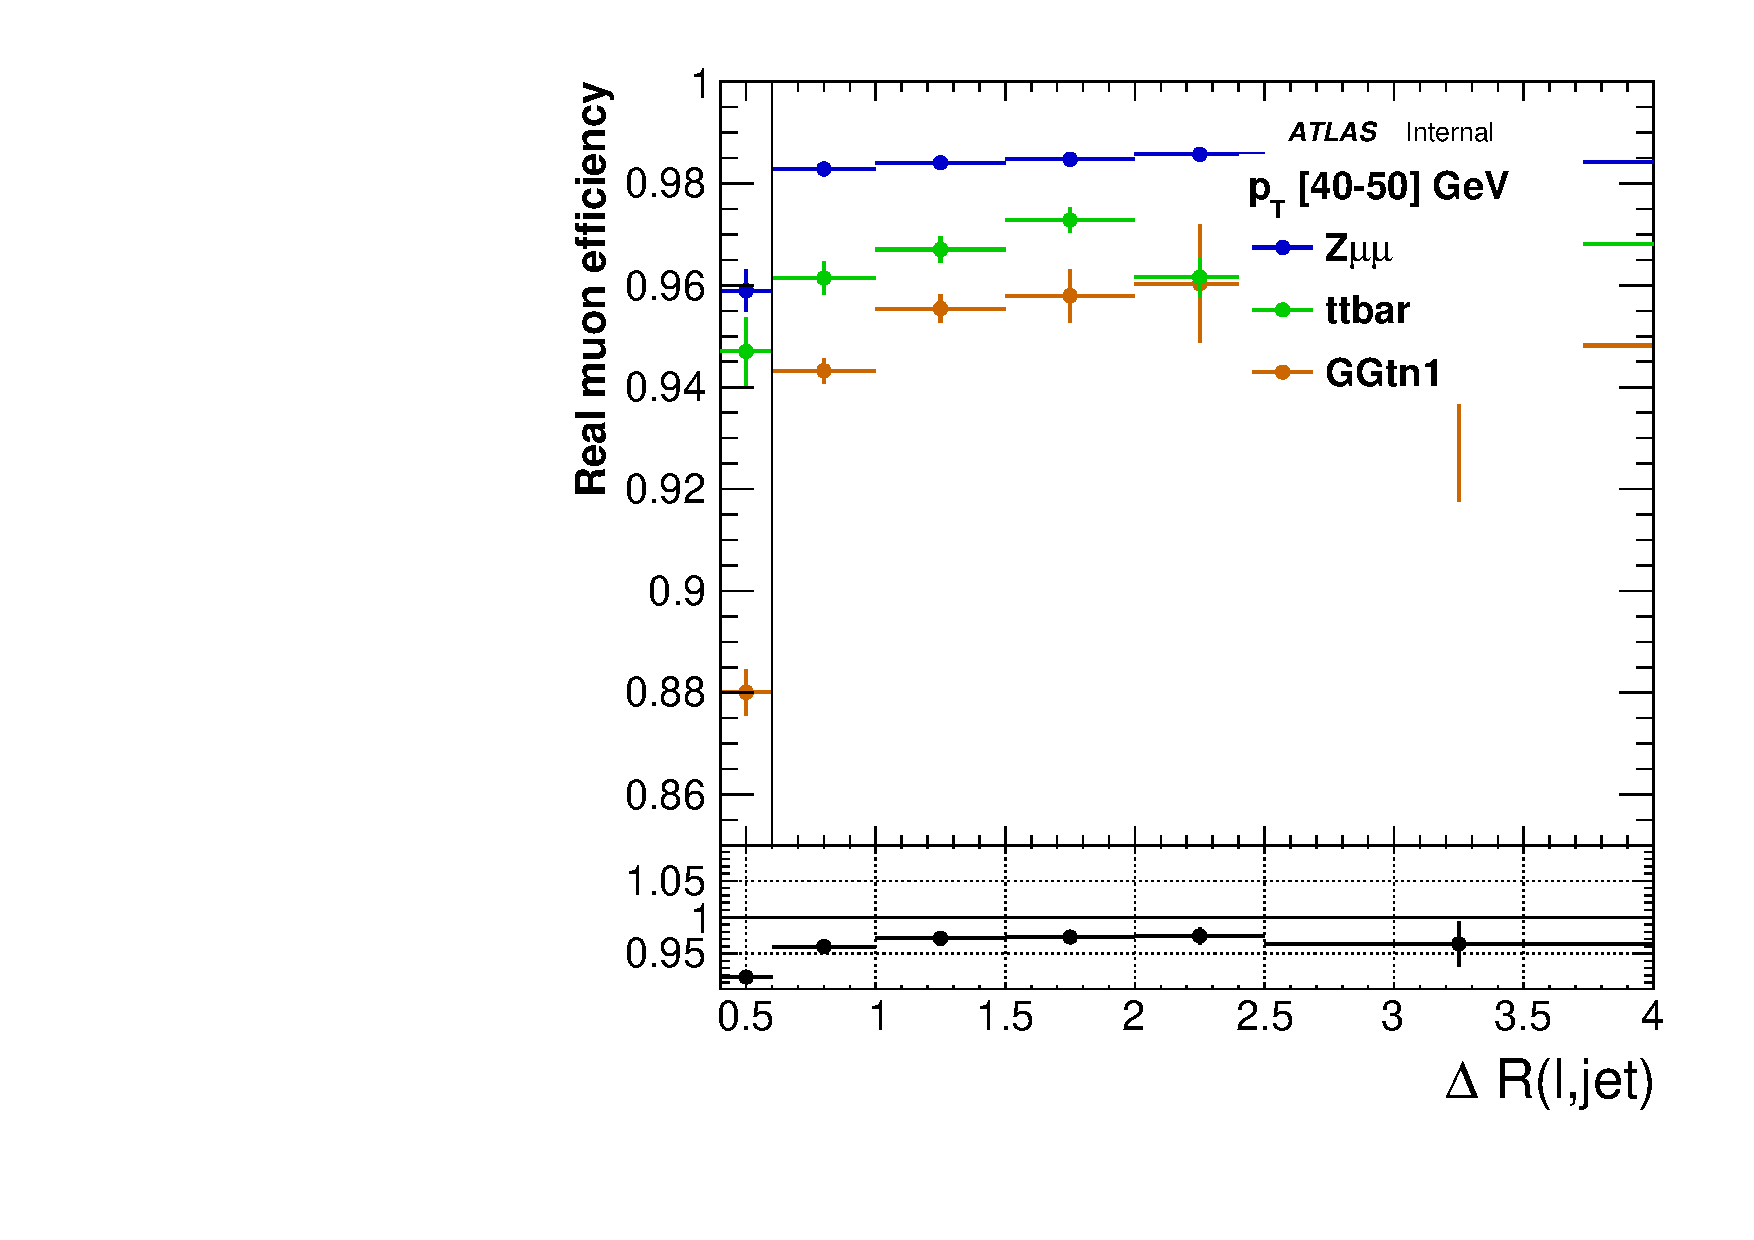
\includegraphics[width=0.3\textwidth]{BKG/realEff/Syst/Syst_Topo_RealEfficiencies_Vs_DRjet_muonspt_range_40_50.pdf} 
	   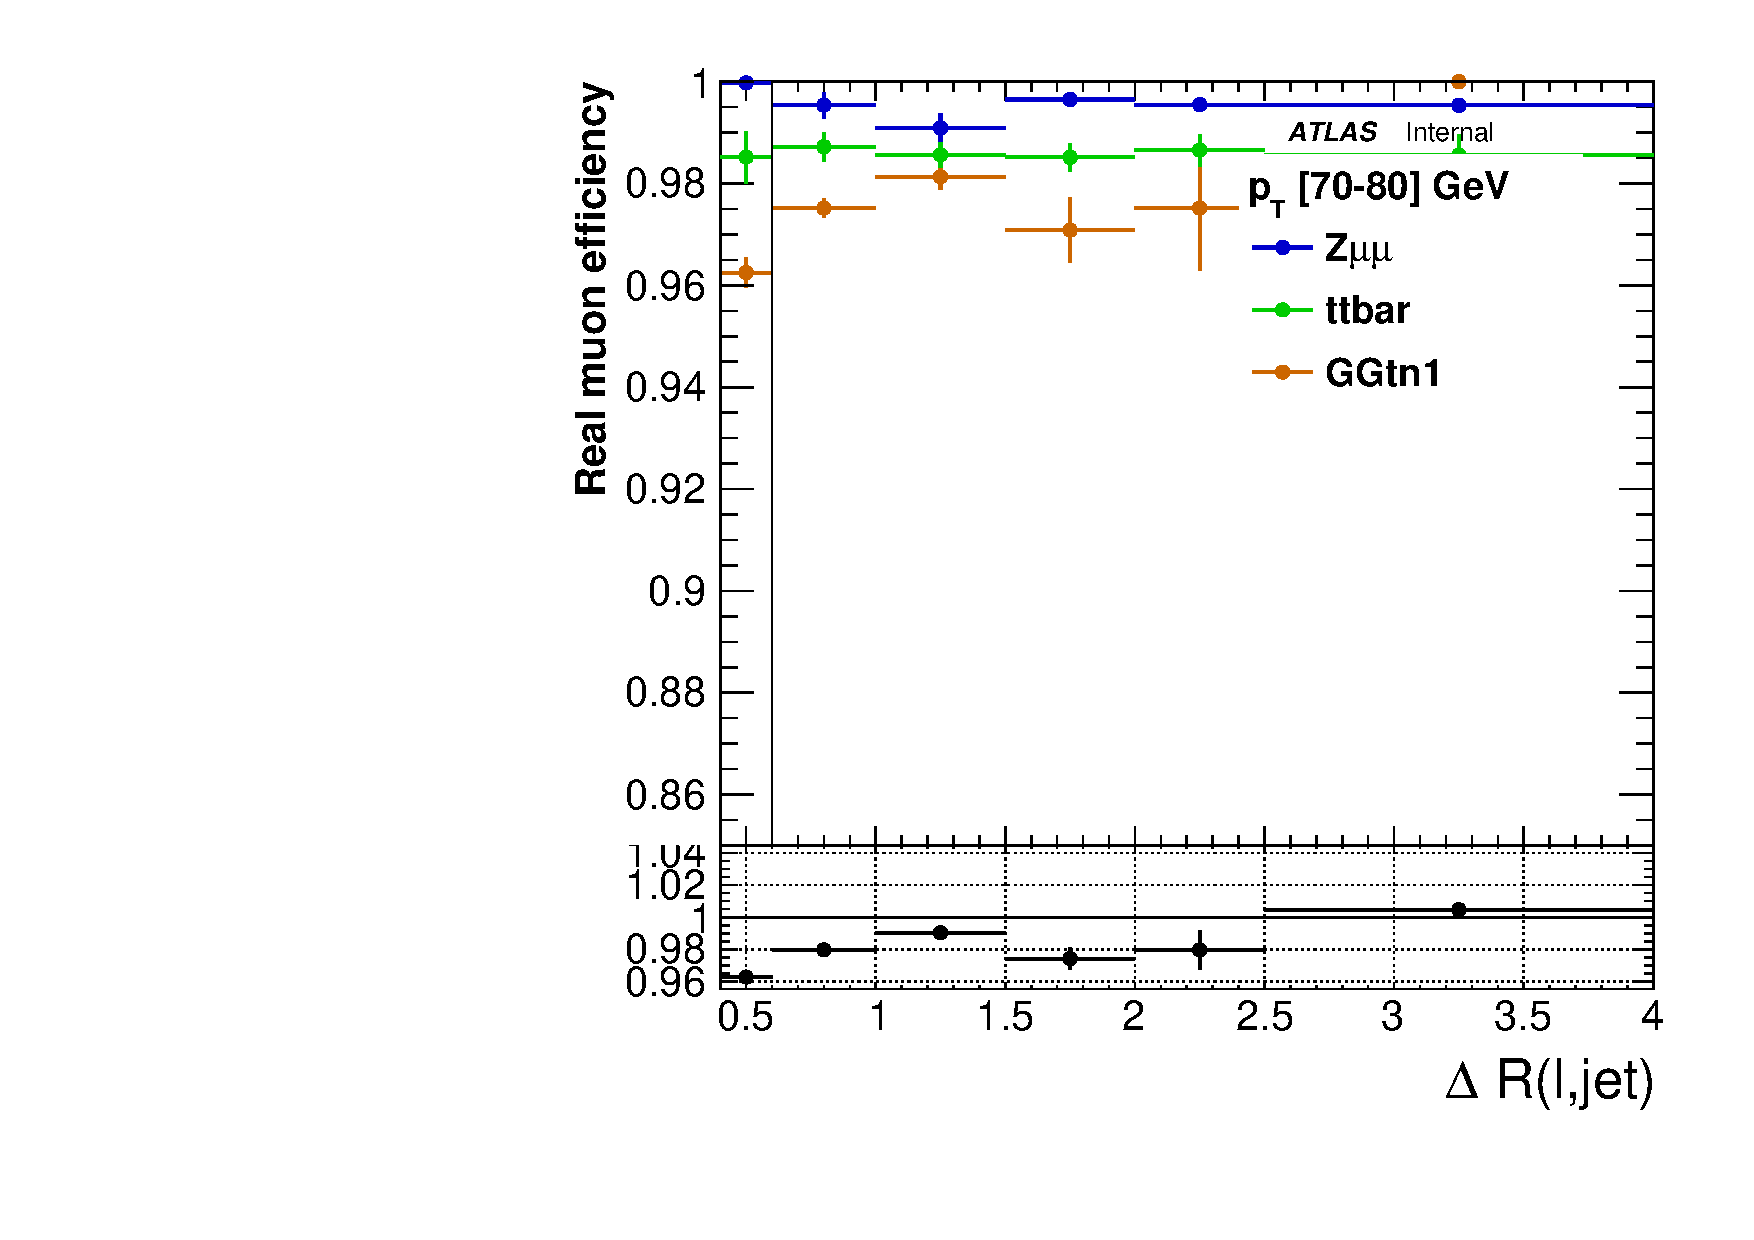
\includegraphics[width=0.3\textwidth]{BKG/realEff/Syst/Syst_Topo_RealEfficiencies_Vs_DRjet_muonspt_range_70_80.pdf}
	   \caption{\label{fig:Syst_Eff_Vs_DRjet} Real electron electrons (top) and muons (bottom) efficiencies as a function of $\Delta R(\ell,\mathrm{jet})$ computed for three different $\pt$ ranges. The left plots correspond to the [15-20] GeV range, the middle to the [40-50] GeV, and the right ones to the [70-80] GeV $\pt$ range. Three processes are considered, $Z\rightarrow ll$ (blue), $t\overline{t}$ (green) and  $\tilde{g}\tilde{g} \rightarrow t\overline{t}t\overline{t} \tilde{\chi}^0_1 \tilde{\chi}^0_1$ with $m_{\tilde{g}} - m_{\tilde{\chi}^0_1} > 1000$ GeV (orange). Prompt leptons are selected using a loose truth match and no \pt reweighing is applied. }
	\end{center}
\end{figure}	
%%%%%%%%%%%%%%%%%%%%%%%%%%%%%%%%%%%%%%%%%%%%%%%%%%%%%%%%%%%		
		
        The efficiency differences as a function of $\Delta R(\ell,\mathrm{jet})$ are then considered for each measurement \pt bin without \pt reweighing to get as close as possible to the efficiency measurement configuration. A $Z\rightarrow \ell\ell$ to SUSY signal extrapolation systematic uncertainty depending on \pt and $\Delta R(\ell,\mathrm{jet})$ is then proposed and presented in Table \ref{tab:Real_Eff_Syst_DRjet}. The systematic proposal has been validated by verifying that the systematic uncertainties assigned as a function $\pt$ and $\Delta R(\ell,\mathrm{jet})$ covers the $Z\rightarrow ll$ to boosted SUSY signal efficiencies differences seen as a function of $|\eta|$ and $n_{Jets}$\footnote{It it is not the case, the systematic uncertainties are enlarged.}.


%%%%%%%%%%%%%%%%%%%%%%%%%%%%%%%%%%%%%%%%%%%%%%%%%%%%%%%%%%%%
\begin{table}[htb!]
	\begin{center}
	    \begin{tabular}{|l|c|c|}
	     \hline
	     \multicolumn{3}{|c|} {\textbf{electrons}}\\
	     \hline 
	     \hline
         &$0.4 < \Delta R(\ell,\mathrm{jet}) < 0.6$ & $\Delta R(\ell,\mathrm{jet}) > 0.6$\\ 
	     \hline
		 $\pt < 60$ GeV & $8\%$ & $4\%$\\
	     \hline
		 $\pt > 60$ GeV	& $5\%$  & $5\%$\\
	     \hline		 
	     \hline
	     \multicolumn{3}{|c|} {\textbf{muons}} \\  
         \hline
         \hline
         &$0.4 < \Delta R(l,\mathrm{Jet}) < 0.6$ & $\Delta R(\ell,\mathrm{jet}) > 0.6$\\ 
         \hline
         $\pt < 15$ GeV      &    $28\%$  &  $10\%$ \\
         \hline
         $15 < \pt < 35$ GeV &    $18\%$  &  $7\%$ \\ 
         \hline
         $35 < \pt < 50$ GeV &    $10\%$  &  $5\%$  \\  
         \hline
         $50 < \pt < 80$ GeV &    $5\%$   &  $3\%$  \\  
         \hline
         $\pt > 80$ GeV      &    $1\%$   &  $1\%$  \\ 
         \hline
		\end{tabular}
	\end{center}
	\caption{ \label{tab:Real_Eff_Syst_DRjet} Real lepton efficiencies $Z+$Jets to SUSY signal extrapolation systematics. These numbers are computed comparing lepton efficiencies computed on $Z+$Jets events with one computed on gtt signals with $m_{g} - m_{\chi^0_1} > 1000$ GeV (boosted topology).}
\end{table}
%%%%%%%%%%%%%%%%%%%%%%%%%%%%%%%%%%%%%%%%%%%%%%%%%%%%%%%%%%%	
						

		\par{\bf Summary of the real lepton efficiencies systematics \\}
		Table \ref{tab:Real_Eff_Syst_tot} summarizes the relative contributions of the different systematic uncertainties for electron (right column) and muons (left column). The first systematic uncertainty corresponds to the measurement. In the electron case, the three numbers corresponds to the measurements $\eta$ ranges ([0-0.8]/[0.8-1.37]/[1.52-2]), shows that larger measurement uncertainties are observed at large pseudorapidity. As the impact of the bremsstrahlung decreases with \pt, the measurement systematic decreases with \pt. The second electron systematic uncertainty corresponds to the trigger one. As the $\texttt{e12\_lhloose}$ trigger efficiency increases with \pt the trigger systematic decreases with \pt. The last systematic uncertainties corresponds to the signal extrapolation ones, more detail is given in the previous paragraph.

% Comparisons of the differents uncertainties sources
%%%%%%%%%%%%%%%%%%%%%%%%%%%%%%%%%%%%%%%%%%%%%%%%%%%%%%%%%%%%
\begin{table}[htb!]
	\begin{center}
	    \begin{tabular}{|l|c|c|}
	     \hline
	                              & \textbf{electrons}                                    &  \textbf{muons}                   \\
	     \hline
	     \hline
		 $\pt < 15$ GeV       & $5.3/5.2/6.7~(meas) \pm 0~(trig) \pm 8/4~(signal)~\%$ & $1~(meas)   \pm 28/10 ~(signal)~\%$\\
	     \hline                                                                
		 $15 < \pt < 20$ GeV  & $3.0/3.5/4.5~(meas) \pm 0~(trig) \pm 8/4~(signal)~\%$ & $0.5~(meas) \pm 18/7 ~(signal)~\%$\\
	     \hline                                                                                            
		 $20 < \pt < 25$ GeV  & $2.5/2.7/3.4~(meas) \pm 4~(trig) \pm 8/4~(signal)~\%$ & $0.1~(meas) \pm 18/7 ~(signal)~\%$\\
	     \hline                                                                                            
		 $25 < \pt < 30$ GeV  & $1.6/1.7/2.4~(meas) \pm 4~(trig) \pm 8/4~(signal)~\%$ & $0.1~(meas) \pm 18/7 ~(signal)~\%$\\
	     \hline                                                                                            
		 $30 < \pt < 35$ GeV  & $0.9/1.3/1.7~(meas) \pm 2~(trig) \pm 8/4~(signal)~\%$ & $0.1~(meas) \pm 18/7 ~(signal)~\%$\\
	     \hline                                                                            
		 $35 < \pt < 40$ GeV  & $0.5/0.8/1.0~(meas) \pm 2~(trig) \pm 8/4~(signal)~\%$ & $0.1~(meas) \pm 10/5 ~(signal)~\%$\\
	     \hline                                                                                            
		 $40 < \pt < 50$ GeV  & $0.2/0.3/0.4~(meas) \pm 2~(trig) \pm 8/4~(signal)~\%$ & $0.1~(meas) \pm 10/5 ~(signal)~\%$\\
	     \hline                                                                            
		 $50 < \pt < 60$ GeV  & $0.2/0.1/0.2~(meas) \pm 1~(trig) \pm 8/4~(signal)~\%$ & $0.1~(meas) \pm 5/3 ~(signal)~\%$\\
	     \hline                                                                                            
		 $60 < \pt < 80$ GeV  & $0/0/0.4~(meas)     \pm 0.5~(trig) \pm 5~(signal)~\%$ & $0.1~(meas) \pm 5/3 ~(signal)~\%$\\
	     \hline                                                                            
		 $\pt > 80$ GeV       & $0.1/0.20.3/~(meas) \pm 0.5~(trig) \pm 5~(signal)~\%$ & $0.1~(meas) \pm 1 ~(signal)~\%$\\
	     \hline
	\end{tabular}
        \end{center}
	\caption{ \label{tab:Real_Eff_Syst_tot} Summary of the systematic uncertainties. The first uncertainties corresponds to the tag-and-probe method measurement method ($meas$). Thee values are given for electrons as corresponding to the three $|\eta|$ measurements ranges ([0-0.8]/[0.8-1.37]/[1.52-2]). The second electron uncertainty correspond to the di-electron trigger bias ($trig$). And the last ones to the $Z\rightarrow \ell\ell$ to SUSY signal extrapolation uncertainty ($signal$). Two values are given corresponding to the following $\Delta R(\ell,\mathrm{jet})$ : [0.4-0.6] / $\Delta R(\ell,\mathrm{jet}) > 0.6$}
\end{table}
%%%%%%%%%%%%%%%%%%%%%%%%%%%%%%%%%%%%%%%%%%%%%%%%%%%%%%%%%%%	

                                                                   

       \par{\bf $Z$ tag-and-probe efficiencies tables \\}

       Tables \ref{tab:Real_Eff_electrons}, \ref{tab:Real_Eff_muons} shows the summary of the electron and muons efficiencies used for the matrix method fake estimates. The first systematic uncertainties corresponds to the statistical ones and are negligible with respect to the seconds ones that corresponds to the systematic ones. 


% Electron efficiency tables
%%%%%%%%%%%%%%%%%%%%%%%%%%%%%%%%%%%%%%%%%%%%%%%%%%%%%%%%%%%%
\begin{table}[htb!]
	\begin{center}
\begin{tabular}{|c|c|c|c|}
\hline 
\textbf{\textbackslash{}pt (GeV) \textbackslash{} $|\eta|$} & \textbf{{[}0-0.8{]}} & \textbf{{[}0.8-1.37{]}} & \textbf{{[}1.52-2{]}}\tabularnewline
\hline 
\hline 
\textbf{{[}10-15{]}} & $43.7\pm0.8\pm4.2/2.9~\%$ & $53.6\pm0.8\pm5.1/3.5~\%$ & $49.6\pm0.8\pm5.2/3.9~\%$\tabularnewline
\hline 
\textbf{{[}15-20{]}} & $56.0\pm0.4\pm4.8/2.8~\%$ & $59.4\pm0.5\pm5.2/3.2~\%$ & $59.8\pm0.5\pm5.5/3.6~\%$\tabularnewline
\hline 
\textbf{{[}20-25{]}} & $64.7\pm0.3\pm6.0/4.0~\%$ & $64.7\pm0.3\pm6.1/4.1~\%$ & $68.0\pm0.3\pm6.5/4.5~\%$\tabularnewline
\hline 
\textbf{{[}25-30{]}} & $70.7\pm0.2\pm6.4/4.2~\%$ & $70.8\pm0.2\pm6.4/4.2~\%$ & $73.6\pm0.2\pm6.8/4.5~\%$\tabularnewline
\hline 
\textbf{{[}30-35{]}} & $75.9\pm0.1\pm6.3/3.5~\%$ & $74.6\pm0.2\pm6.2/3.5~\%$ & $78.7\pm0.2\pm6.8/3.7~\%$\tabularnewline
\hline 
\textbf{{[}35-40{]}} & $80.0\pm0.1\pm6.6/3.6~\%$ & $76.8\pm0.1\pm6.4/3.5~\%$ & $79.8\pm0.2\pm6.6/3.7~\%$\tabularnewline
\hline 
\textbf{{[}40-50{]}} & $82.9\pm0.1\pm6.8/3.7~\%$ & $79.8\pm0.1\pm6.6/3.6~\%$ & $84.1\pm0.1\pm6.9/3.8~\%$\tabularnewline
\hline 
\textbf{{[}50-60{]}} & $86.9\pm0.1\pm7.0/3.6~\%$ & $83.9\pm0.2\pm6.8/3.5~\%$ & $87.0\pm0.2\pm7.0/3.6~\%$\tabularnewline
\hline 
\textbf{{[}60-80{]}} & $90.7\pm0.2\pm4.6/4.6~\%$ & $89.2\pm0.2\pm4.5/4.5~\%$ & $89.6\pm0.4\pm4.5/4.5~\%$\tabularnewline
\hline 
\textbf{$\pt>80$}    & $93.8\pm0.2\pm4.7/4.7~\%$ & $90.3\pm0.5\pm4.7/4.7~\%$ & $92.4\pm0.5\pm4.6/4.6~\%$\tabularnewline
\hline 
\end{tabular}
        \end{center}
	\caption{ \label{tab:Real_Eff_electrons} Electron efficiencies tables. The first and the second uncertainties are the statistical and the systematic one respectively. The shown systematic uncertainties ($syst$) corresponds to the quadratic sum of the tag-and-probe, trigger and the signal extrapolation systematic uncertainties. Two values are given corresponding to the two signal extrapolation systematic  $\Delta R(\ell,\mathrm{jet})$ ranges : [0.4-0.6] (left) / $\Delta R(\ell,\mathrm{jet}) > 0.6$ (right) range.}
\end{table}
%%%%%%%%%%%%%%%%%%%%%%%%%%%%%%%%%%%%%%%%%%%%%%%%%%%%%%%%%%%	


% Muon efficiency tables
%%%%%%%%%%%%%%%%%%%%%%%%%%%%%%%%%%%%%%%%%%%%%%%%%%%%%%%%%%%%
\begin{table}[htb!]
	\begin{center} {\scriptsize
\begin{tabular}{|c|c|c|c|c|}
\hline 
\textbf{\textbackslash{}pt (GeV) \textbackslash{} $|\eta|$} & \textbf{{[}0-0.6{]}} & \textbf{{[}0.6-1.2{]}} & \textbf{{[}1.2-1.8{]}} & \textbf{{[}1.8-2.5{]}}\tabularnewline
\hline 
\hline 
\textbf{{[}10-15{]}} & $84.6\pm0.4~\pm24/8.5~\%$ & $84.6\pm0.4~\pm24/8.5~\%$ & $84.7\pm0.4~\pm24/8.5~\%$ & $83.6\pm0.4~\pm23/8.4~\%$\tabularnewline
\hline 
\textbf{{[}15-20{]}} & $86.4\pm0.2~\pm16/6.1~\%$ & $86.4\pm0.2~\pm16/6.1~\%$ & $85.8\pm0.3~\pm15/6.0~\%$ & $86.1\pm0.3~\pm16/6.0~\%$\tabularnewline
\hline 
\textbf{{[}20-25{]}} & $90.8\pm0.1~\pm16/6.4~\%$ & $90.9\pm0.2~\pm16/6.4~\%$ & $90.6\pm0.2~\pm16/6.3~\%$ & $90.3\pm0.2~\pm16/6.3~\%$\tabularnewline
\hline 
\textbf{{[}25-30{]}} & $93.9\pm0.1~\pm17/6.6~\%$ & $93.7\pm0.1~\pm17/6.6~\%$ & $93.2\pm0.1~\pm17/6.5~\%$ & $93.2\pm0.1~\pm17/6.5~\%$\tabularnewline
\hline 
\textbf{{[}30-35{]}} & $95.6\pm0.1~\pm17/6.7~\%$ & $95.3\pm0.1~\pm17/6.7~\%$ & $95.0\pm0.1~\pm17/6.7~\%$ & $94.6\pm0.1~\pm17/6.6~\%$\tabularnewline
\hline 
\textbf{{[}35-40{]}} & $97.2\pm O(0.1)~\pm9.7/4.9~\%$ & $97.3\pm O(0.1)~\pm9.7/4.9~\%$ & $97.0\pm O(0.1)~\pm9.7/4.8~\%$ & $96.5\pm0.1~\pm9.6/4.8~\%$\tabularnewline
\hline 
\textbf{{[}40-50{]}} & $98.4\pm O(0.1)~\pm9.8/4.9~\%$ & $98.5\pm O(0.1)~\pm9.9/4.9~\%$ & $98.3\pm O(0.1)~\pm9.8/4.9~\%$ & $98.0\pm O(0.1)~\pm9.8/4.9~\%$\tabularnewline
\hline 
\textbf{{[}50-60{]}} & $98.9\pm O(0.1)~\pm4.9/3.0~\%$ & $99.0\pm O(0.1)~\pm5.0/3.0~\%$ & $98.9\pm O(0.1)~\pm4.9/3.0~\%$ & $98.7\pm O(0.1)~\pm4.9/3.0~\%$\tabularnewline
\hline 
\textbf{{[}60-70{]}} & $99.2\pm O(0.1)~\pm5.0/3.0~\%$ & $99.3\pm O(0.1)~\pm5.0/3.0~\%$ & $99.2\pm O(0.1)~\pm5.0/3.0~\%$ & $99.0\pm O(0.1)~\pm5.0/3.0~\%$\tabularnewline
\hline 
\textbf{{[}70-80{]}} & $99.5\pm O(0.1)~\pm5.0/3.0~\%$ & $99.5\pm O(0.1)~\pm5.0/3.0~\%$ & $99.4\pm O(0.1)~\pm5.0/3.0~\%$ & $99.2\pm0.1~\pm5.0/3.0~\%$\tabularnewline
\hline 
$\pt>80$ & $99.5\pm0.1\pm1.0/1.0~\%$ & $99.5\pm0.1\pm1.0/1.0~\%$ & $99.5\pm0.1\pm1.0/1.0~\%$ & $99.5\pm0.1\pm1.0/1.0~\%$\tabularnewline
\hline 
\end{tabular}}
	\caption{ \label{tab:Real_Eff_muons} Muon efficiencies tables. The first and the second uncertainties are the statistical and the systematic one respectively. The shown systematic uncertainties ($syst$) corresponds to the quadratic sum of the tag-and-probe and the signal extrapolation systematic uncertainties. Two values are given corresponding to the two signal extrapolation systematic  $\Delta R(\ell,\mathrm{jet})$ ranges : [0.4-0.6] (left) / $\Delta R(\ell,\mathrm{jet}) > 0.6$ (right) range.}
        \end{center}
\end{table}
%%%%%%%%%%%%%%%%%%%%%%%%%%%%%%%%%%%%%%%%%%%%%%%%%%%%%%%%%%%


%%%%%%%%%%%%%%%%%%
% SUBSECTION 4
%%%%%%%%%%%%%%%%%%
	\subsection{Real leptons efficiency measured using $t\overline{t}$ events}
	\label{App:RealEff_ttbar_TandP}	
	\par{\bf Presentation of the method \\}
	In order to have an efficiency measurement as close to the signal region as possible, a tag-and-probe method has been put in place to select leptons from $t\overline{t}$ events. \\
	The selection of the $t\overline{t}$ events is based on the following criteria :
	\begin{itemize}
		\item Exactly two baseline leptons with a $p_{T}$ larger than 30 GeV are requested. This brings rejection against $W+jets$, $t\overline{t}Z$, tri-bosons or other complex processes.		
		\item A least one b-jet (using the b-jet definitions from the analysis) is required. This brings rejection against $Z$/$W+jets$ and $VV$ events.
		\item A $E_{T}^{miss} >$ 30 GeV requirement is added if the two selected leptons are $ee$ or $\mu\mu$. This brings further rejection against $Z$+$jets$ events and other background events.
		\item A $Z$ veto removing lepton pairs with 70 $< m_{ll} <$ 100 GeV is also applied if the two selected leptons are $ee$ or $\mu\mu$ to bring further rejection against $Z$+$jets$ and $t\overline{t}Z$ events.
	\end{itemize}
	One of the two leptons is requested to pass the signal lepton requirements (tag lepton) and the other to pass the baseline requirements (probe lepton). The two leptons are alternatively considered as possible tag with no restrictions on the lepton flavour. 
		
		
	\par{\bf Validation of the method \\}
	The effect of $t\overline{t}$ event selection cuts are shown in Table \ref{tab:ttbar_TandP_Cutflow}. This table shows that the W+jet events are mainly rejected by the exactly 2 leptons with $p_{T} >$ 30 GeV requirement and the at least one b-jet requirements. On the other hand the $Z+jet$ background is rejected by the at least one b-jet, the $E_T^{miss}$ and the $m_{\mathrm{ll}}$ veto requirements. After all selection cuts, the contribution from the V+jets events represents $\sim2\%$ of the $t\overline{t}$ statistics assessing a good purity in the $t\overline{t}$ tag-and-probe events selection. $VV$ and $t\overline{t}V$ are contributing much less due to their lower cross sections. The exactly two baseline lepton requirement is further reducing the contribution from $VV$ and $t\overline{t}V$ by selecting events with two lepton in the final state. The contribution from $VV$ processes is further rejected with the at least one $b-jet$ requirement. The contribution from $t\overline{t}Z$ processes is further reduced by the $m_{\mathrm{ll}}$ veto. Marginal contribution are expected from $t\overline{t}t\overline{t}$ due to their low cross section and the at exactly two baseline lepton requirement.
		
%%%%%%%%%%%%%%%%%%%%%%%%%%%%%%%%%%%%%%%%%%%%%%%%%%%%%%%%%%%%	
\begin{table}[htb!]
  	\begin{center} 
    		\begin{tabular}{|l|c|c|c|} \hline
				Processes    &   $t\overline{t}$  &  $W$+$jets$   &  $Z$+$jets$ \\ \hline \hline
				At least 2 baseline leptons & 82106 & 38181  & 3519252 \\ 
				Exactly 2 baseline leptons with $p_T >$ 30 GeV & 39375 ($48\%$) & 3451 ($9\%$) & 2861459 ($81\%$) \\
				At least 1 b-jet            & 32242 ($82\%$) & 70 ($2\%$) & 36174 ($1.2\%$) \\
				$E_T^{miss} >$ 30 GeV ($ee$/$\mu\mu$)   & 29950 ($93\%$) & 63 ($90\%$) &9 514 ($26\%$)\\
				$m_{\mathrm{ll}}$ veto                           & 26969 ($90\%$) & 54 ($86\%$) & 766 ($8\%$)\\ \hline
				Yields normalized to $t\overline{t}$ events& 100$\%$ & 0.06$\%$ & 2$\%$\\ \hline
		    \end{tabular}
			\caption{\label{tab:ttbar_TandP_Cutflow} Expected number of events for 3 $\textnormal{fb}^{-1}$ computed that passes the $t\overline{t}$ tag-and-probe events cuts. The yields corresponding to the $t\overline{t}$ processes (first column) are computed using a $t\overline{t}$ Monte Carlo simulation with filter that removes all hadronic decays, the ones corresponding to the W+jets processes (second column) are computed using $W \rightarrow e/\mu/\tau~\nu_{e/\mu/\tau}$ Monte Carlo simulations and ones corresponding to the $Z$+$jets$ (third column) are computed using $Z \rightarrow ee/\mu\mu/\tau\tau$ Monte Carlo simulations. The last row corresponds to the final number of events for the different processes normalized to the number of remaining $t\overline{t}$ events.}
    	\end{center}
    \end{table}		
%%%%%%%%%%%%%%%%%%%%%%%%%%%%%%%%%%%%%%%%%%%%%%%%%%%%%%%%%%%%	

% 	$p_{T}$, $\eta$ and the $\Delta R(\ell,\mathrm{jet})$ distributions with and without additional loose truth match has been compared using a $t\overline{t}$ Monte Carlo sample. good agreement is observed.\\			
% 	
% 	% T&P+truth & T&P Real eff comparison ttbar
% 	The top (middle) plots from Figure \ref{fig:CheckTandP_RealEff_ttbar} show the real efficiencies as a function of the $p_T$ ($\eta$) of the electron (left) and the muons (right). The real electrons efficiencies computed without truth match are $1-2\%$ lower than the ones computed with truth match depending on the $p_T$ and $\eta$ range. The real electron efficiencies differences are larger at low $p_T$ and large $\eta$. The real muon efficiencies agree within $\sim1\%$ for $p_T >$ 40 GeV and perfect agreement is reached for $p_T >$ 60 GeV. The electron and muons real efficiencies differences are mainly due to non-prompt leptons identified as probe leptons (ex : an electron coming from a b-jet).
% 			
% %%%%%%%%%%%%%%%%%%%%%%%%%%%%%%%%%%%%%%%%%%%%%%%%%%%%%%%%%%%%					
% 	\begin{figure}[!htb]
% 	  \begin{center} 
% 	   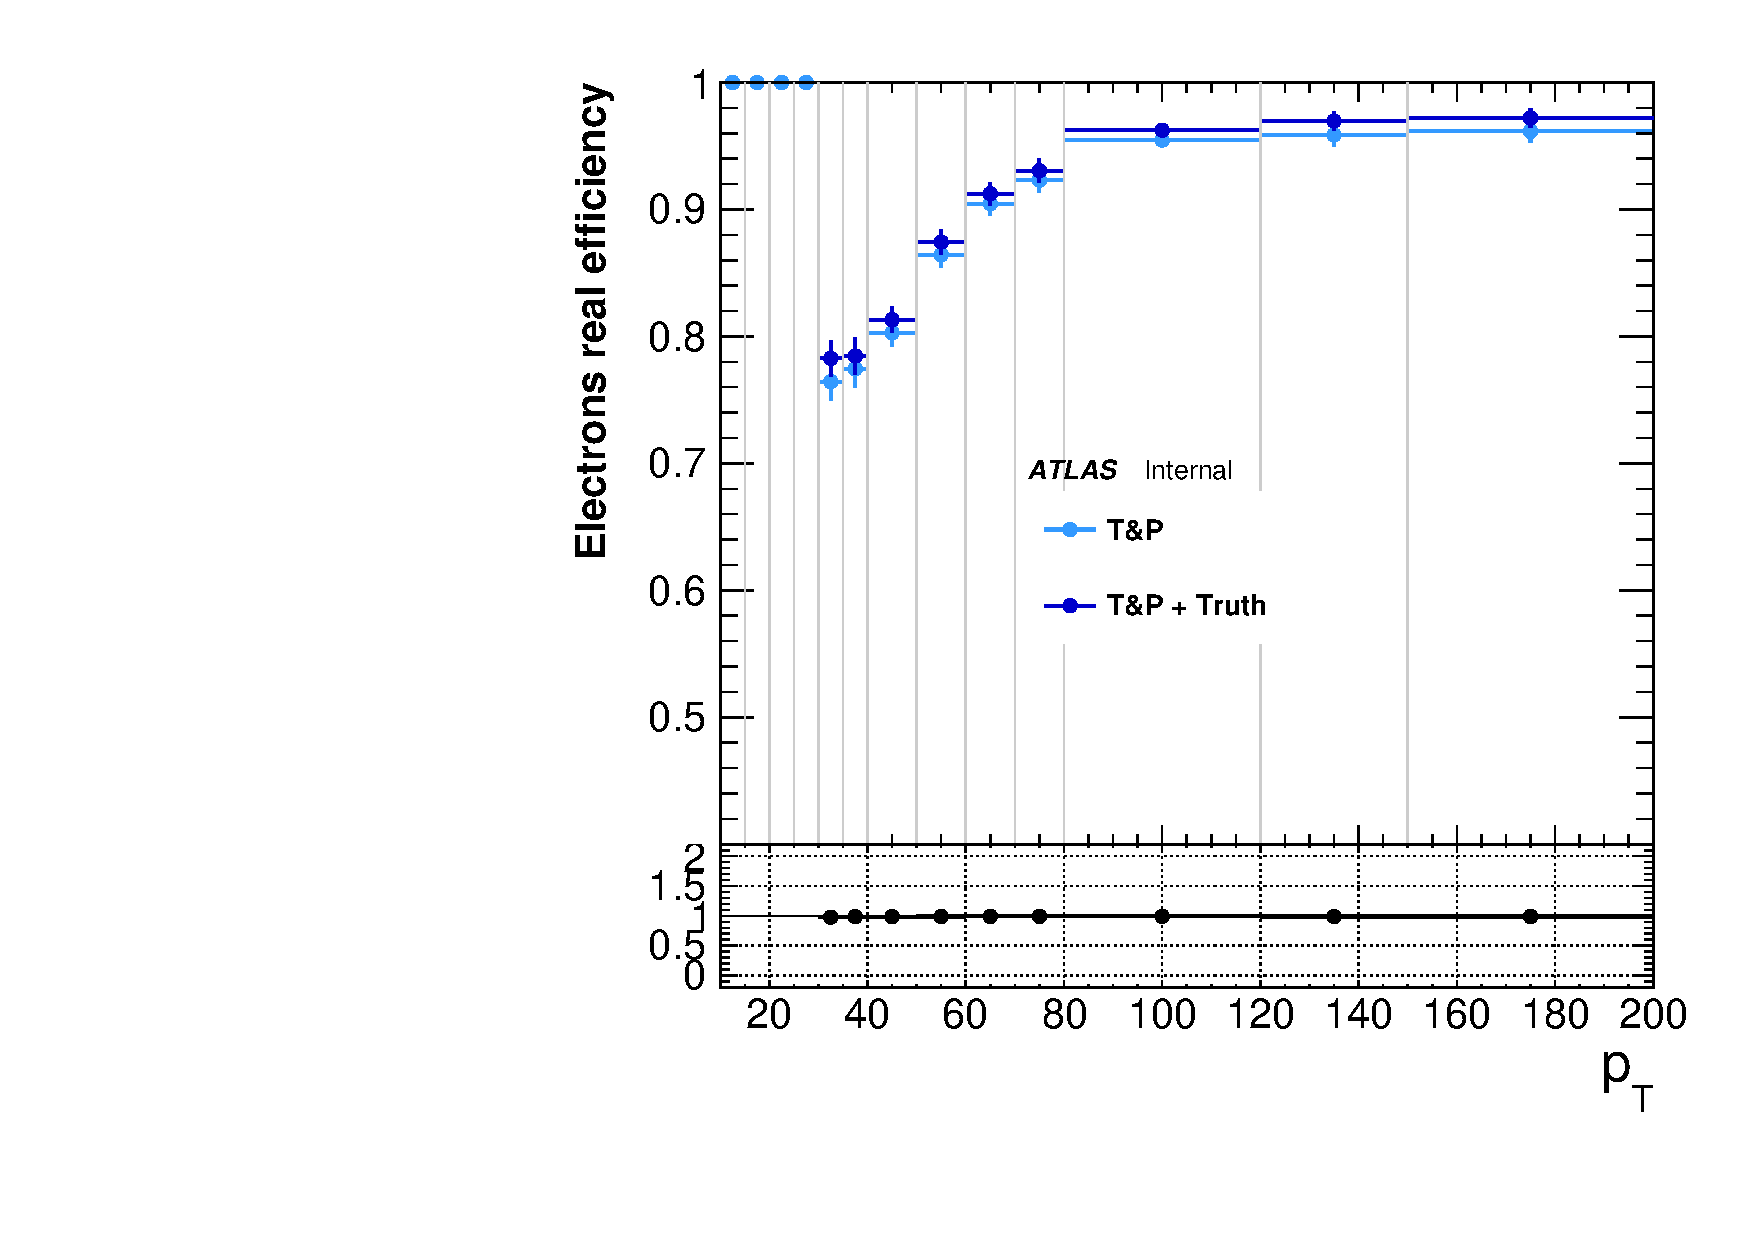
\includegraphics[width=0.4\textwidth]{BKG/realEff/Truth_Checks/25ns_ttbar_CheckTandP_RealEfficiencies_Vs_pt_electrons.pdf} 
% 	   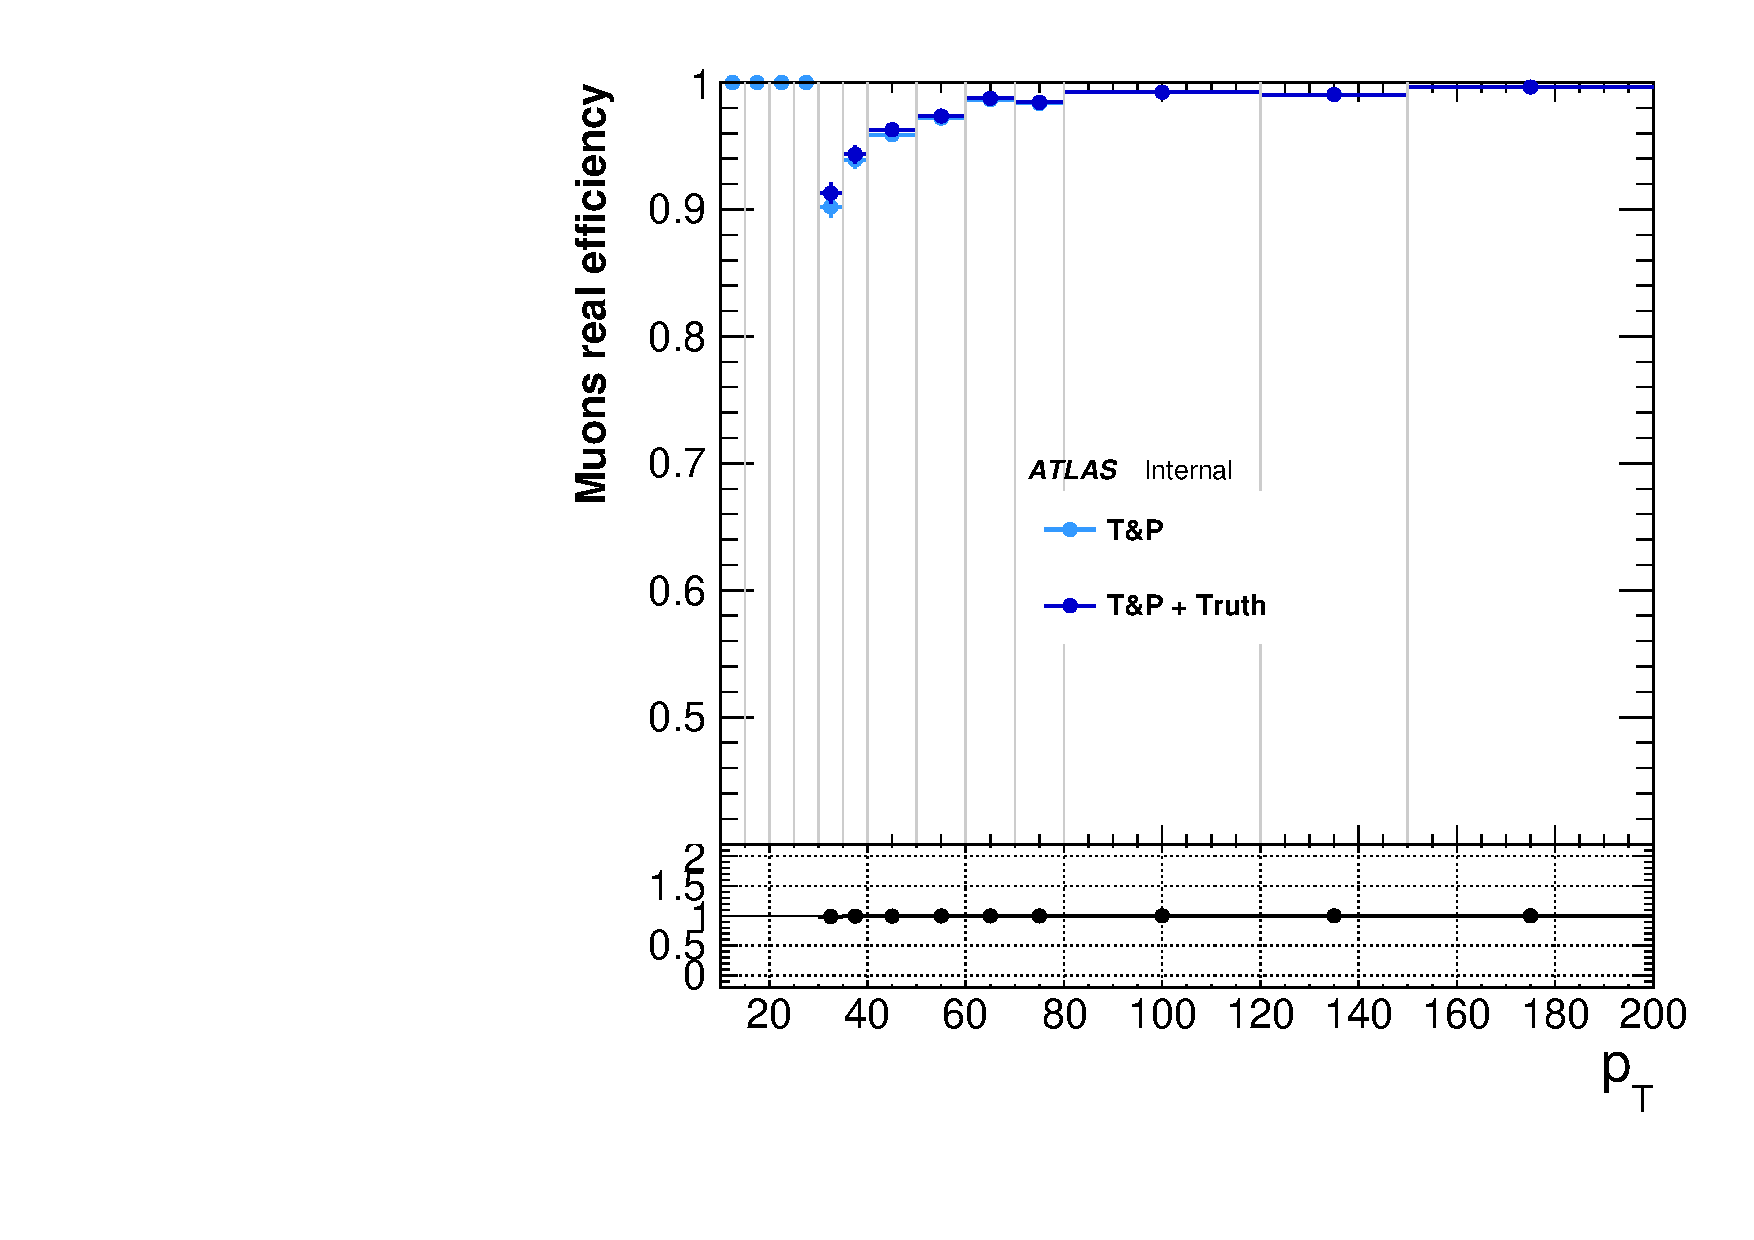
\includegraphics[width=0.4\textwidth]{BKG/realEff/Truth_Checks/25ns_ttbar_CheckTandP_RealEfficiencies_Vs_pt_muons.pdf} 
% 	   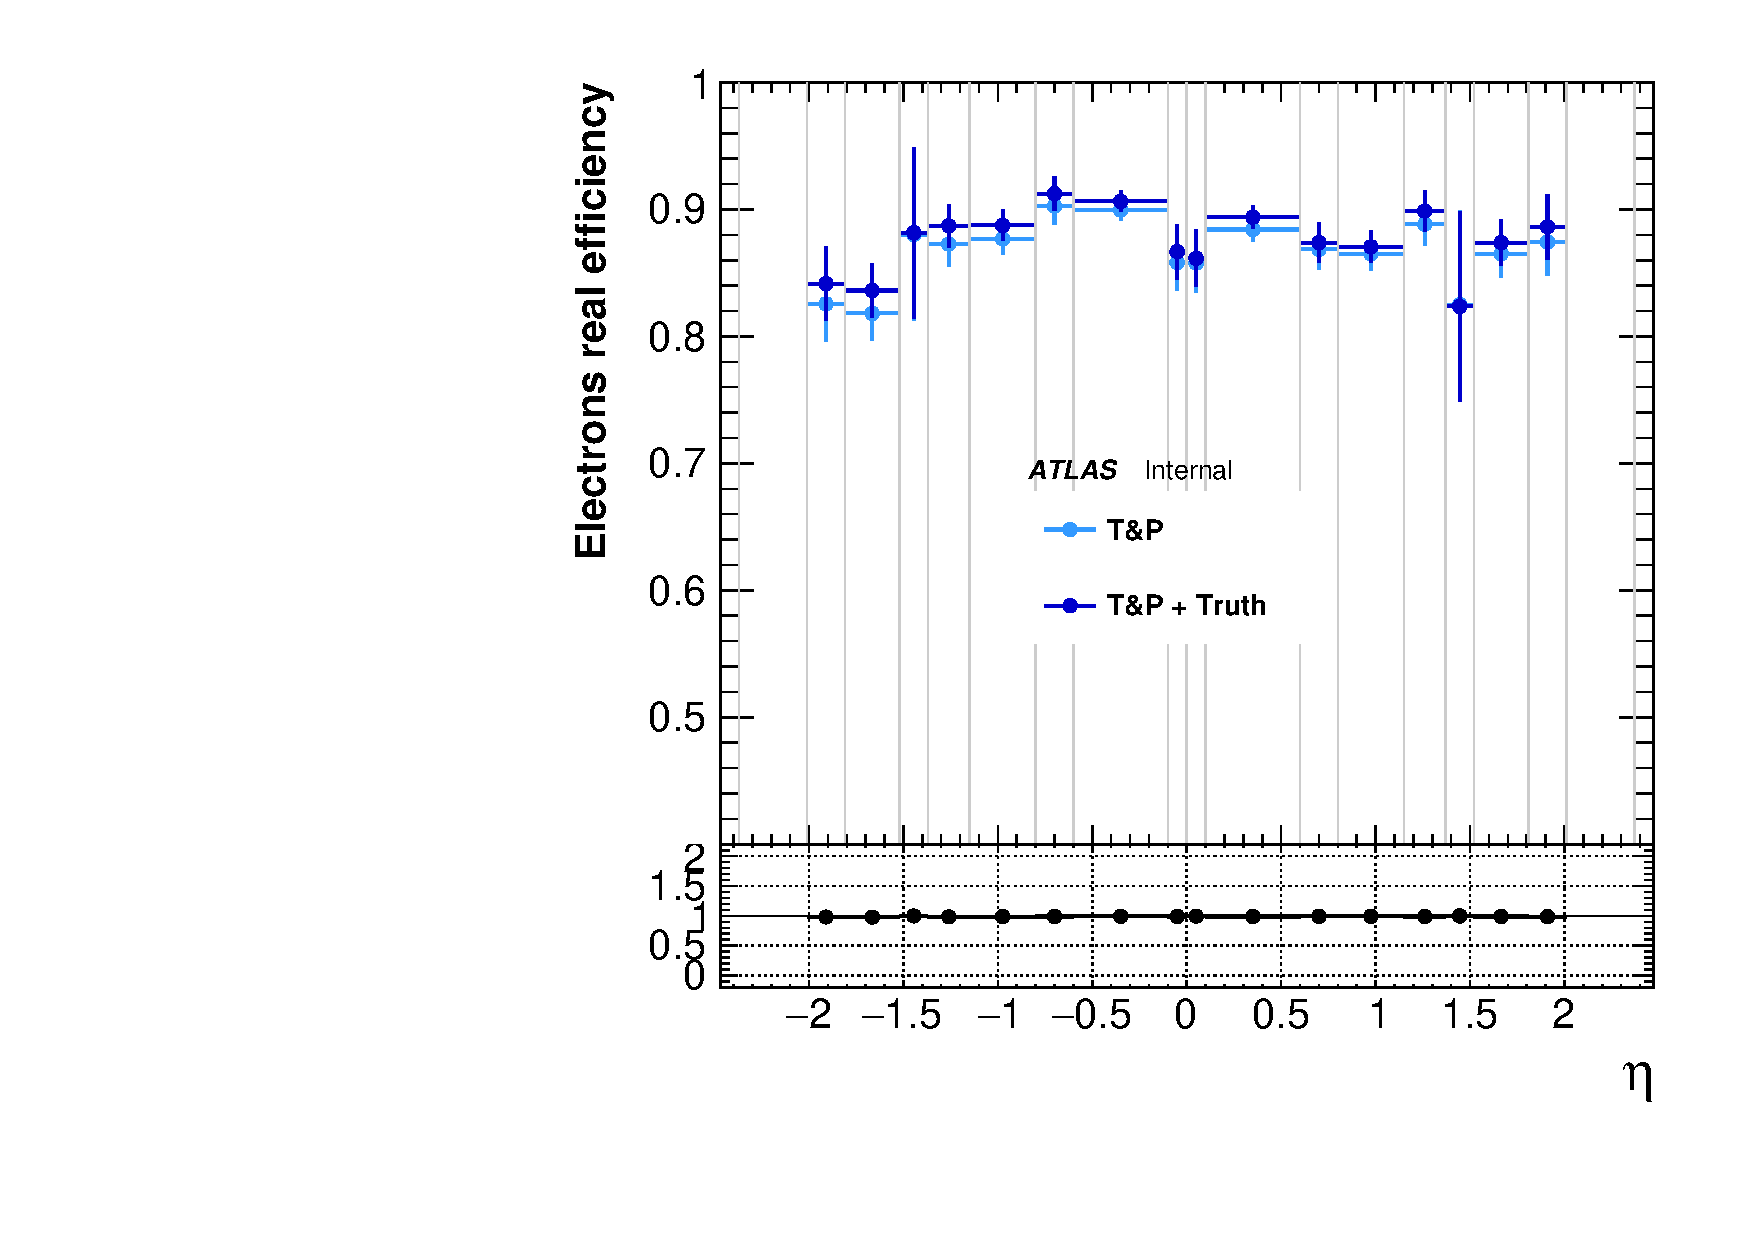
\includegraphics[width=0.4\textwidth]{BKG/realEff/Truth_Checks/25ns_ttbar_CheckTandP_RealEfficiencies_Vs_eta_electrons.pdf} 
% 	   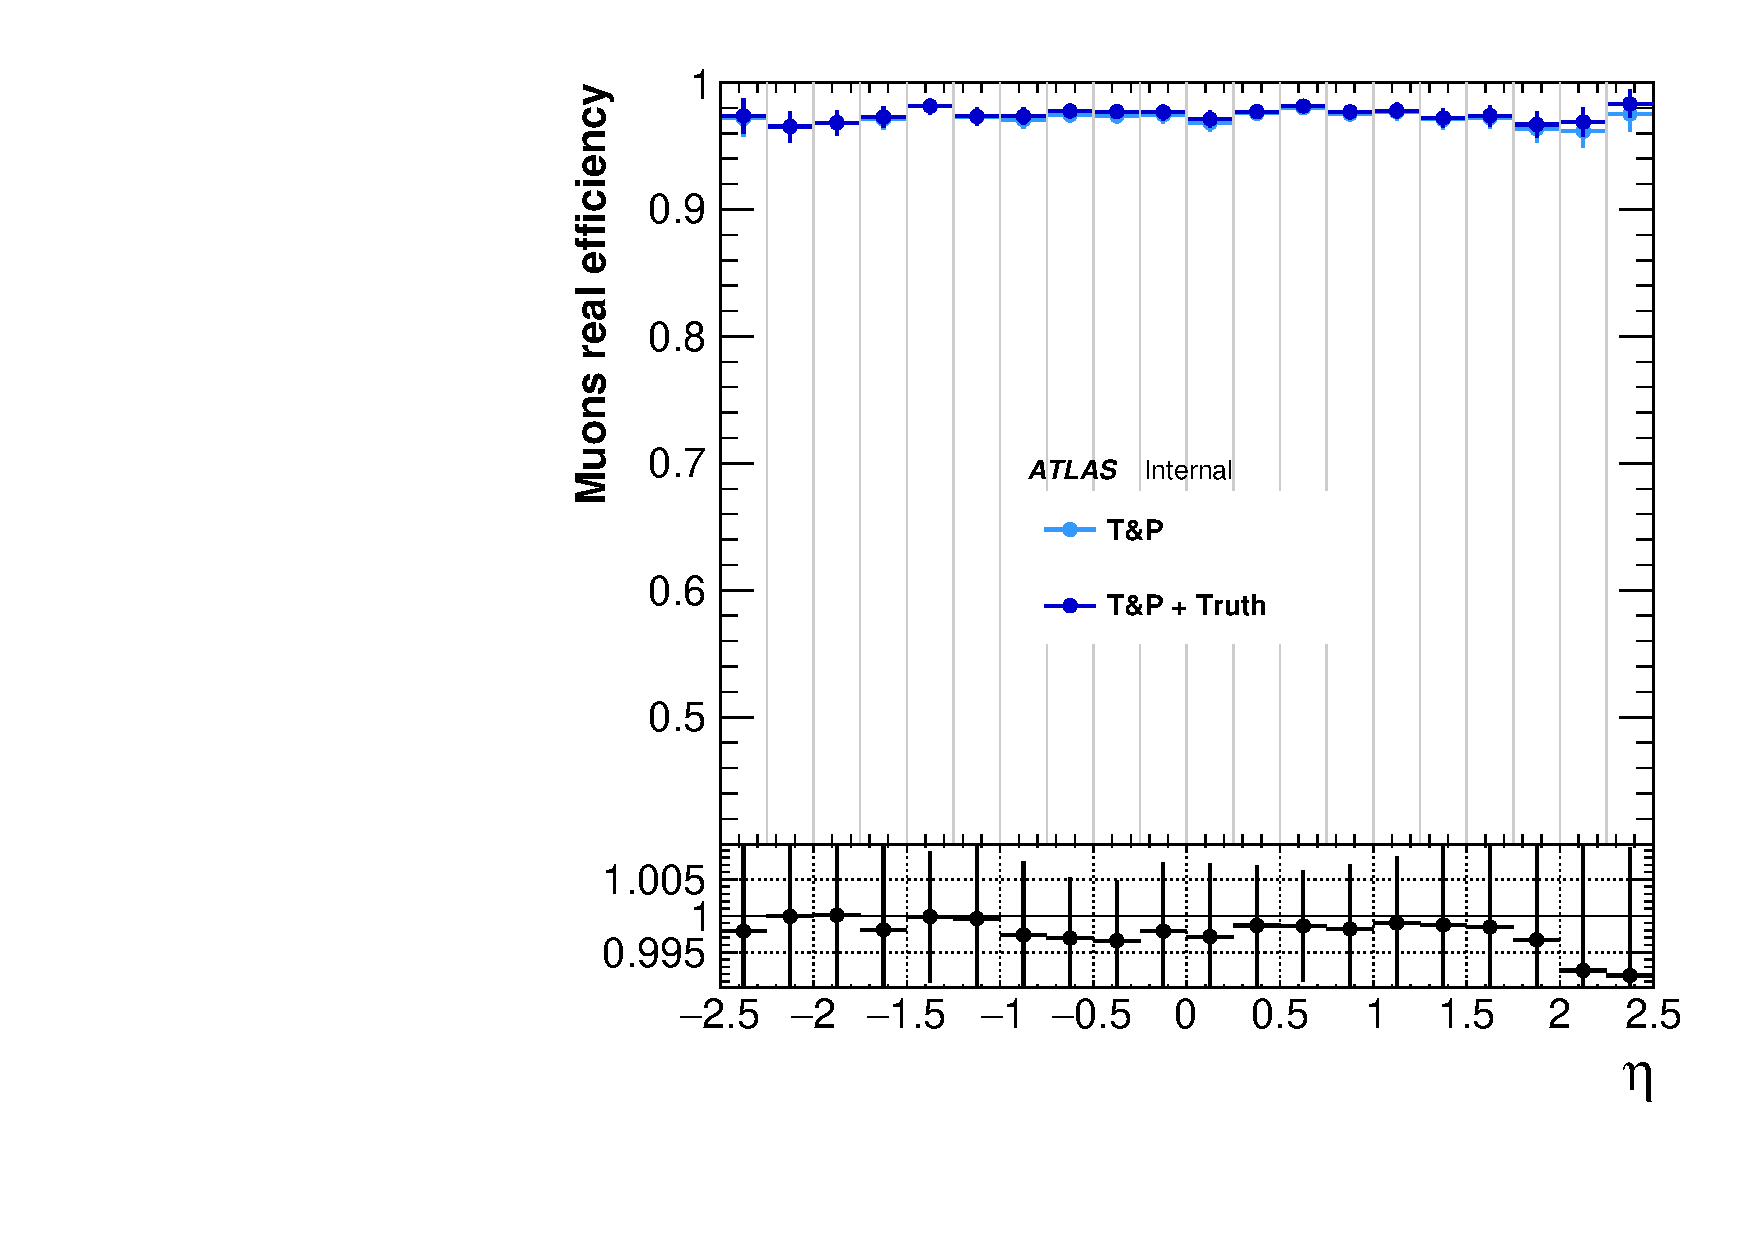
\includegraphics[width=0.4\textwidth]{BKG/realEff/Truth_Checks/25ns_ttbar_CheckTandP_RealEfficiencies_Vs_eta_muons.pdf} 
% 	   \caption{\label{fig:CheckTandP_RealEff_ttbar} Real leptons efficiencies computed using the $t\overline{t}$ tag-and-probe method as a function of $p_{T}$ (top), $\eta$ (bottom). These efficiencies has been computed using a $t\overline{t}$ Monte Carlo sample, with (dark blue) and without (dark blue) a lepton truth match. The left plots are corresponding to electrons and the right plots to muons. A loose truth match has been used for the electron to recover the contributions from FSR and electrons that has emitted a converted bremsstrahlung photon.}
% 	  \end{center}
% 	\end{figure}	
% %%%%%%%%%%%%%%%%%%%%%%%%%%%%%%%%%%%%%%%%%%%%%%%%%%%%%%%%%%%%	

	
	\par{\bf Results \\}	
	The distributions and the real lepton efficiencies computed with probes leptons extracted in data using the $t\overline{t}$ tag-and-probe method have been compared to the ones from simulated $t\overline{t}$ processes. All scale factors, the pile-up reweighing have been applied for Monte Carlo and the Monte Carlo distributions are normalised to the data. The full 2015 data is used for those measurements which corresponds to an integrated luminosity of $\sim3.2~\mathrm{fb}^{-1}$ after good run list requirements.
	Figure \ref{fig:Data_Vs_MC_RealEff_ttbar} shows the comparison between the real lepton efficiency computed with the $t\overline{t}$ tag-and-probe using data and $t\overline{t}$ simulated events. The real efficiency is computed for different bins in $\pt$ (top), $|\eta|$ (middle) and $\Delta R(\ell,\mathrm{jet})$ (bottom). These plots shows that the real lepton efficiencies computed on data agrees within the statistical errors to the ones computed on Monte Carlo. The Monte Carlo efficiencies are very close to the Data ones. The validates the measurement method.


%%%%%%%%%%%%%%%%%%%%%%%%%%%%%%%%%%%%%%%%%%%%%%%%%%%%%%%%%%%%	
	\begin{figure}[!htb]
	  \begin{center} 
	   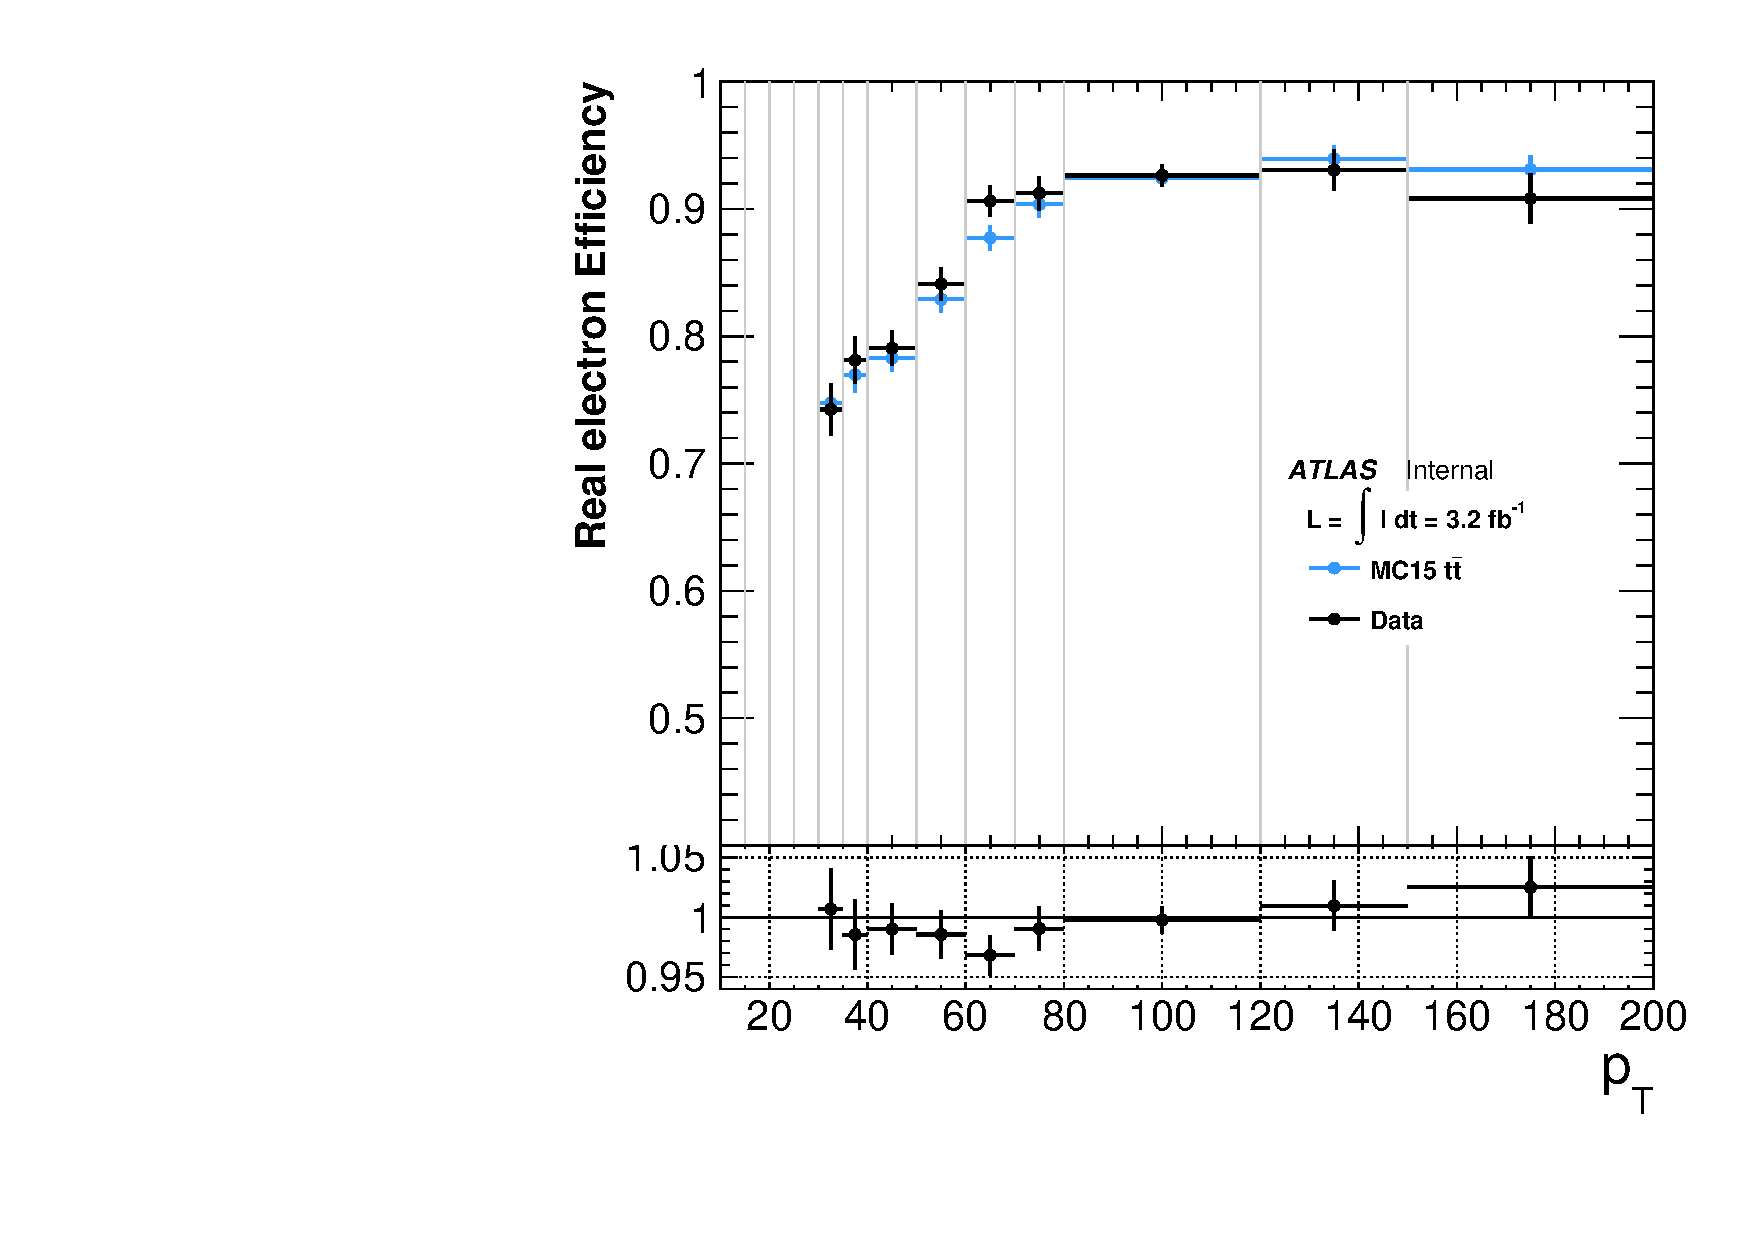
\includegraphics[width=0.3\textwidth]{BKG/realEff/Data_To_MC/Data_Vs_MC15_RealEfficiencies_Vs_pt_electrons_ttbarTandP.pdf} 
	   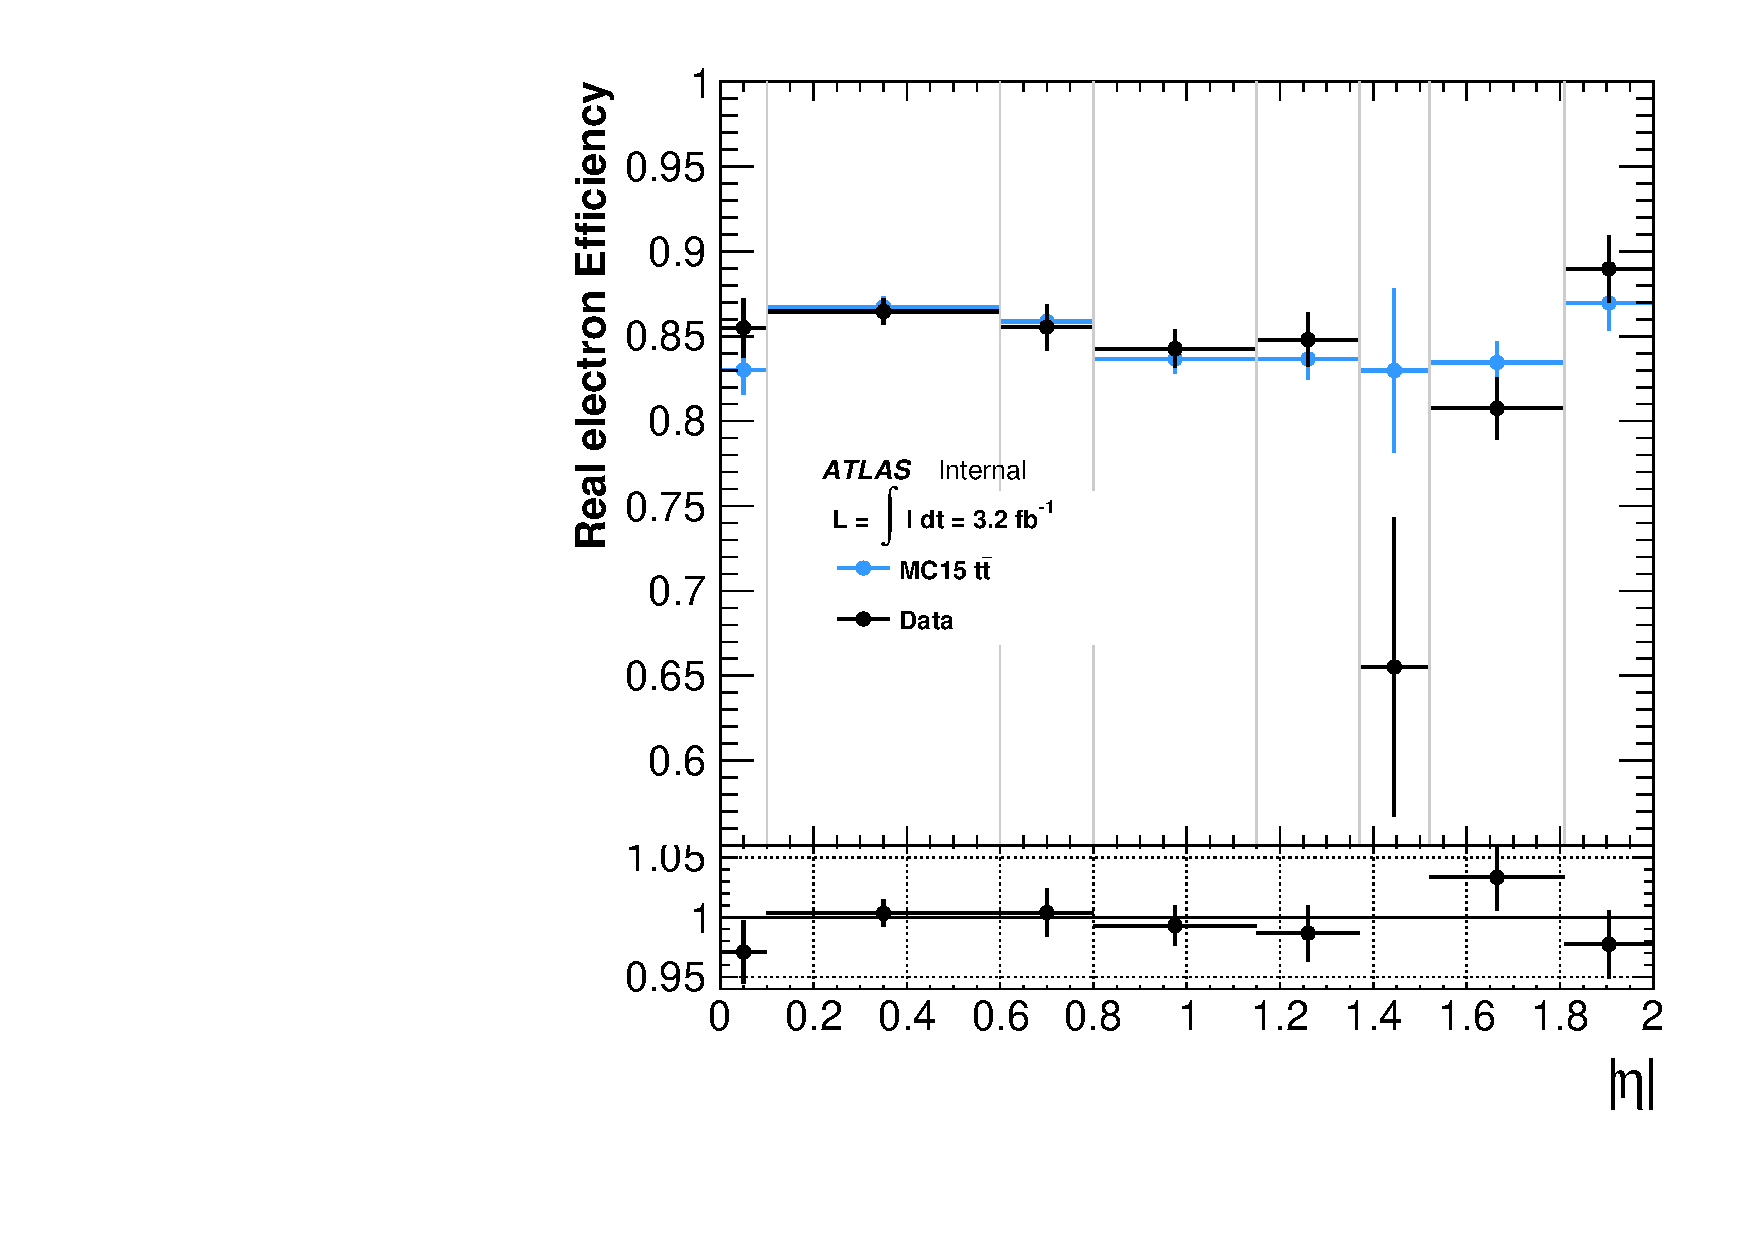
\includegraphics[width=0.3\textwidth]{BKG/realEff/Data_To_MC/Data_Vs_MC15_RealEfficiencies_Vs_eta_electrons_ttbarTandP.pdf} 
	   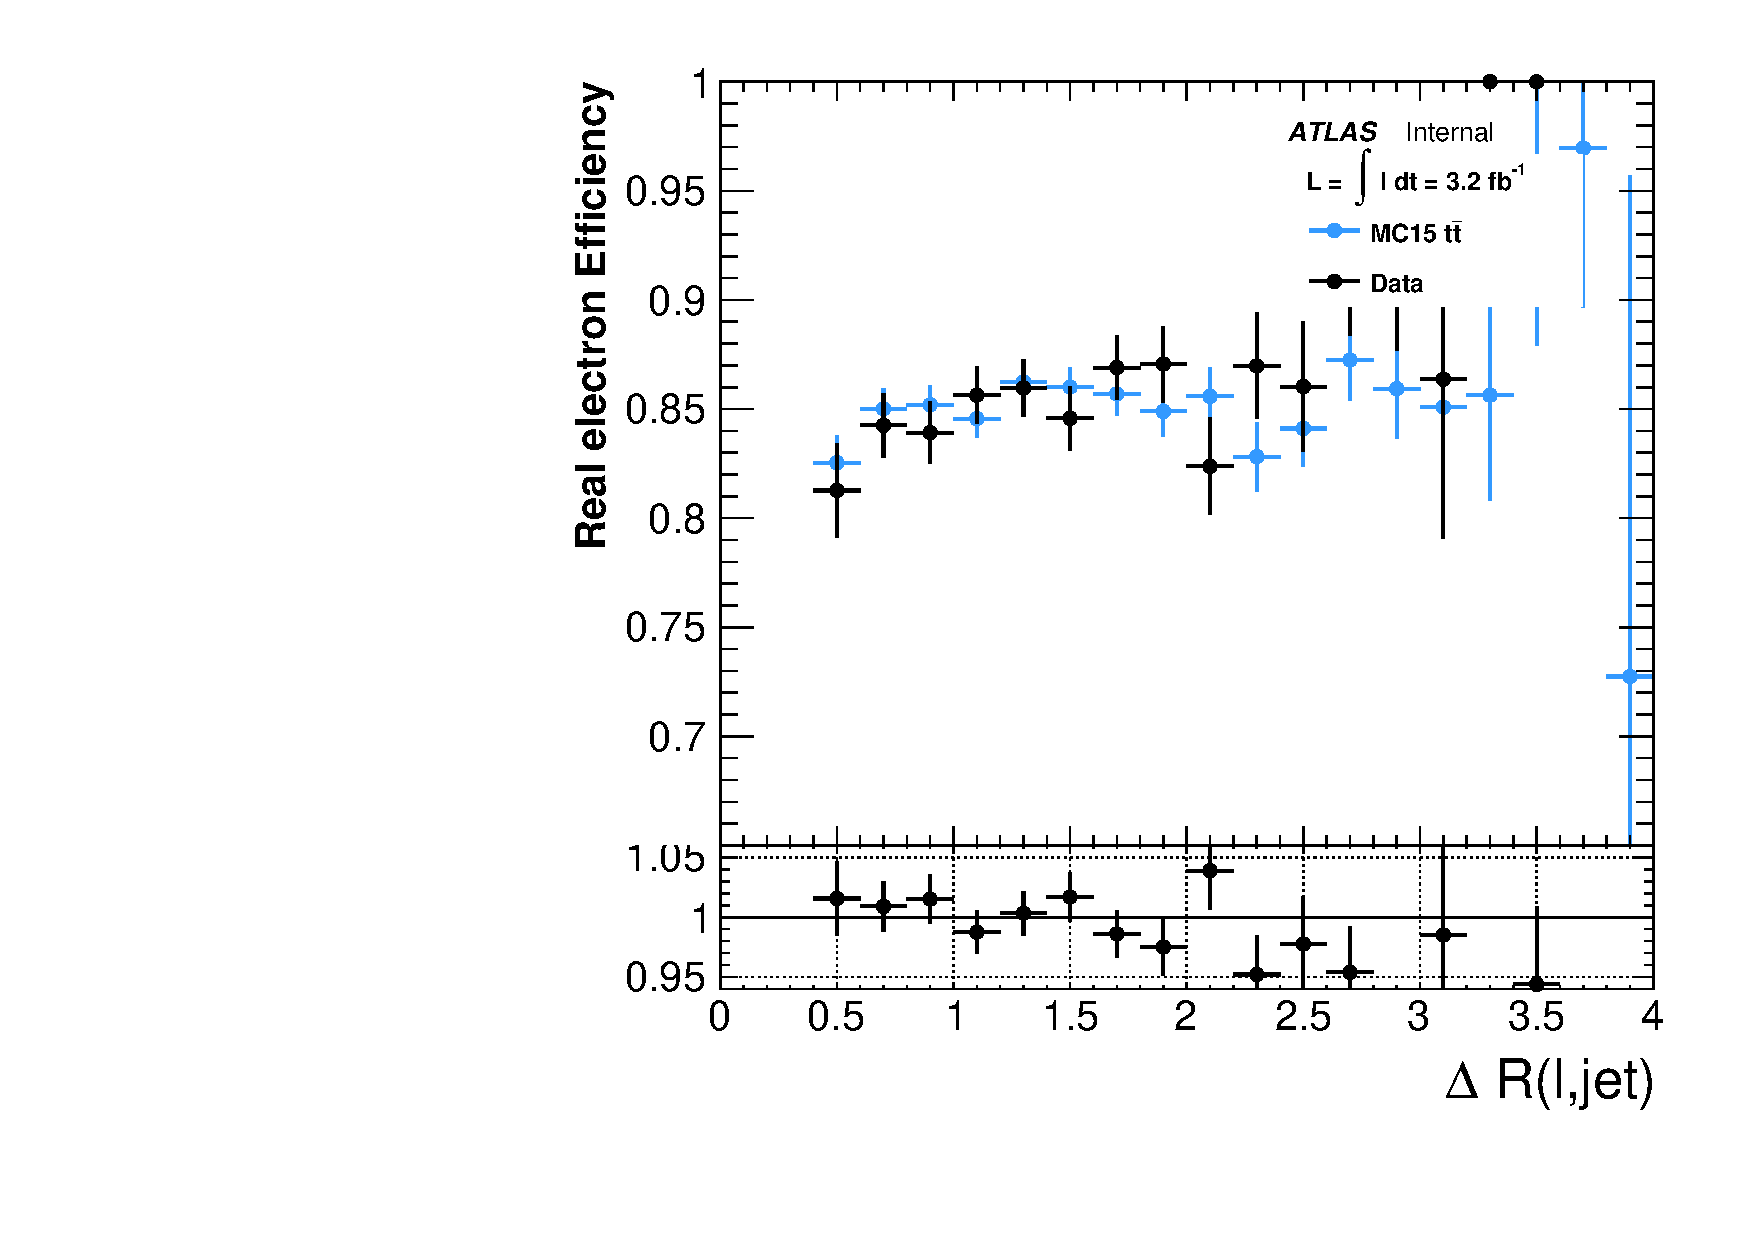
\includegraphics[width=0.3\textwidth]{BKG/realEff/Data_To_MC/Data_Vs_MC15_RealEfficiencies_Vs_DRjet_electrons_ttbarTandP.pdf} 
	   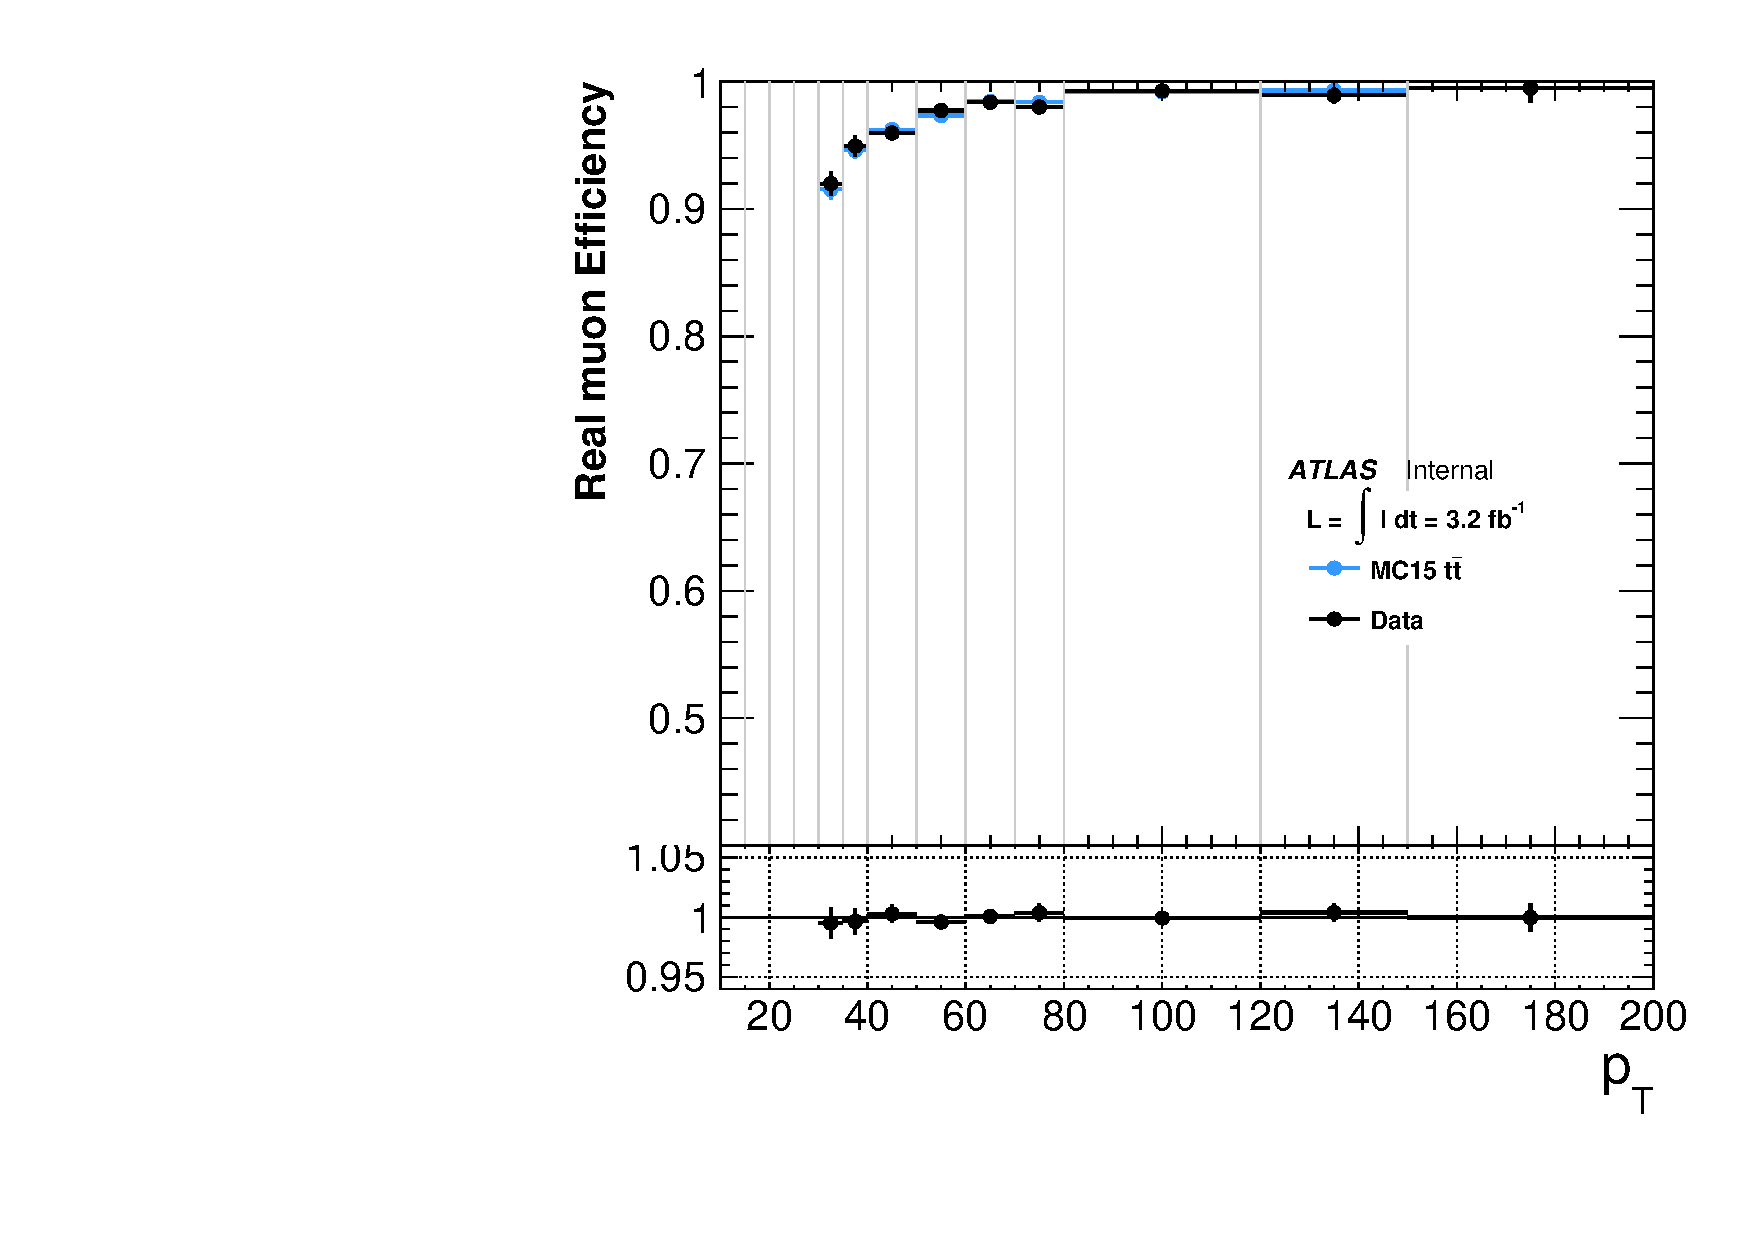
\includegraphics[width=0.3\textwidth]{BKG/realEff/Data_To_MC/Data_Vs_MC15_RealEfficiencies_Vs_pt_muons_ttbarTandP.pdf} 
	   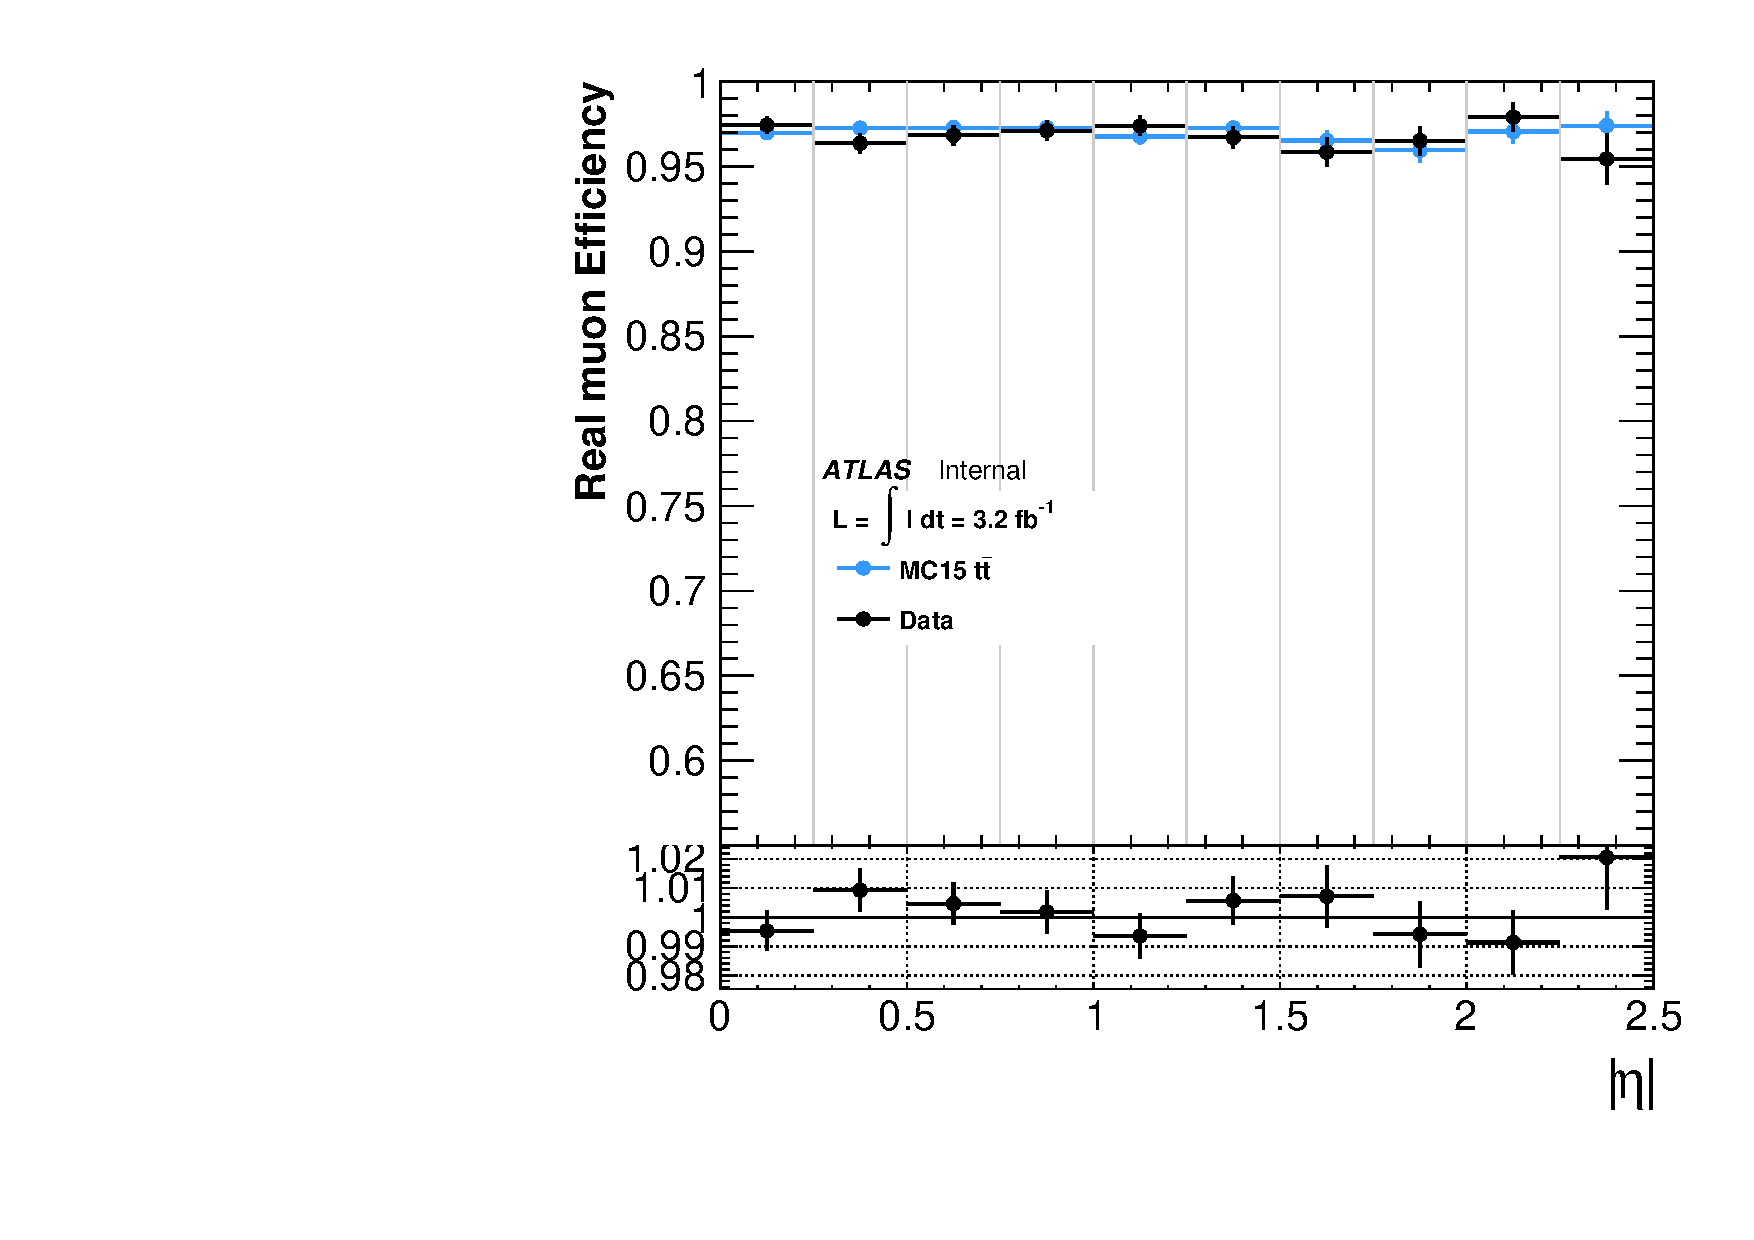
\includegraphics[width=0.3\textwidth]{BKG/realEff/Data_To_MC/Data_Vs_MC15_RealEfficiencies_Vs_eta_muons_ttbarTandP.pdf} 
	   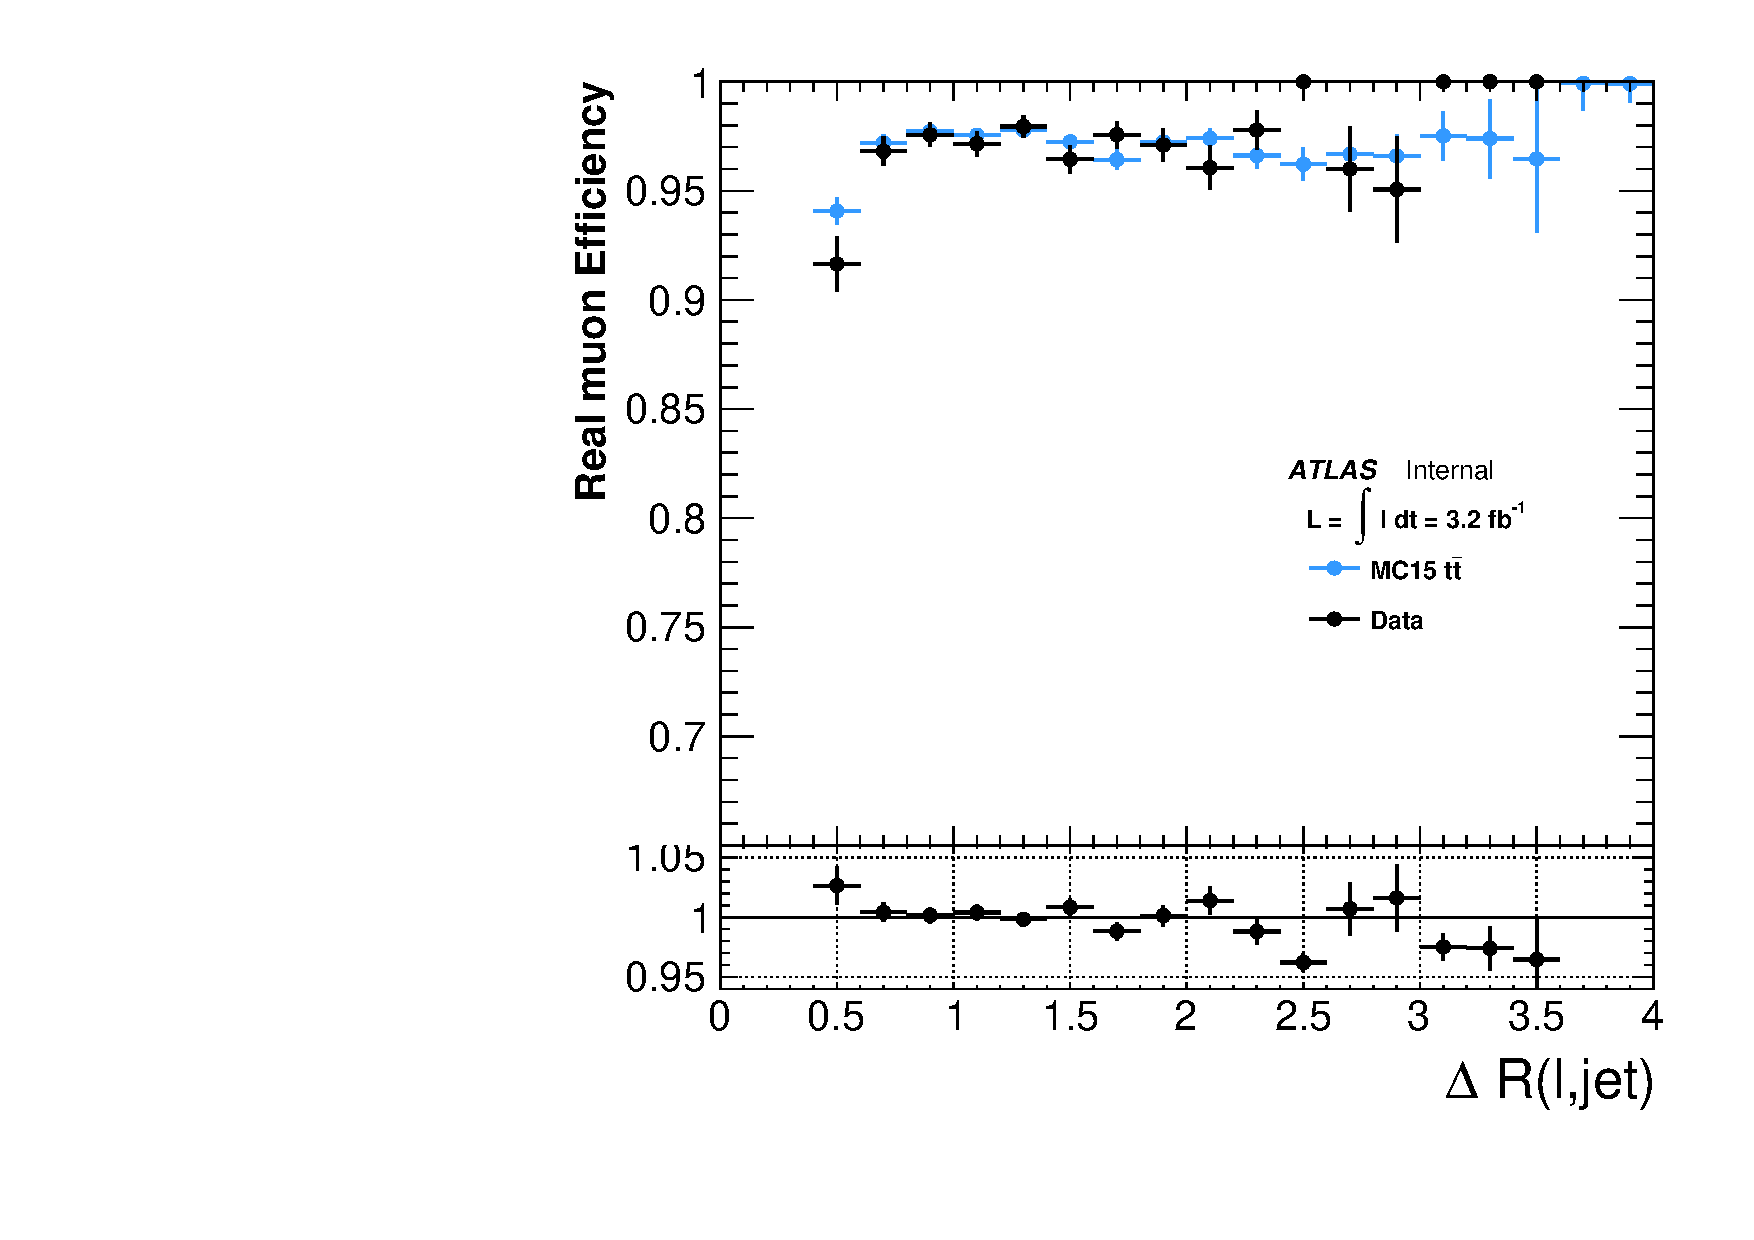
\includegraphics[width=0.3\textwidth]{BKG/realEff/Data_To_MC/Data_Vs_MC15_RealEfficiencies_Vs_DRjet_muons_ttbarTandP.pdf} 
	   \caption{\label{fig:Data_Vs_MC_RealEff_ttbar} Real lepton efficiencies as a function of $p_{T}$ (left), $\eta$ (middle) and $\Delta R(\ell,\mathrm{jet})$ (right) computed using $t\overline{t}$ probe leptons extracted from $t\overline{t}$ Monte Carlo simulations with truth match (light blue) and 2015 data (black points).}
	  \end{center}
	\end{figure}	
%%%%%%%%%%%%%%%%%%%%%%%%%%%%%%%%%%%%%%%%%%%%%%%%%%%%%%%%%%%%	


	\par{\bf Comparison between $Z$ and the $t\overline{t}$ real leptons efficiencies measurements\\}
		The $t\overline{t}$ tag-and-probe method was first developed to enrich the statistics at large $p_T$ and low $\Delta R(\ell,\mathrm{jet})$ for the real leptons efficiency measurements on data. Figure \ref{fig:Z_Vs_ttbar_Cumul_pt_distributions} shows the total number of probe leptons expected to be extracted with the $Z$ and the $t\overline{t}$ tag-and-probe method for $3\textnormal{fb}^{-1}$ of collision data for different $p_T$ threshold. Those plots show that the number of lepton extracted from $Z$ events are 10 times larger than the number of lepton extracted from $t\overline{t}$ at large $\pt$ for both muons and electrons. 
		
%%%%%%%%%%%%%%%%%%%%%%%%%%%%%%%%%%%%%%%%%%%%%%%%%%%%%%%%%%%%	
	\begin{figure}[!htb]
	  \begin{center} 
	   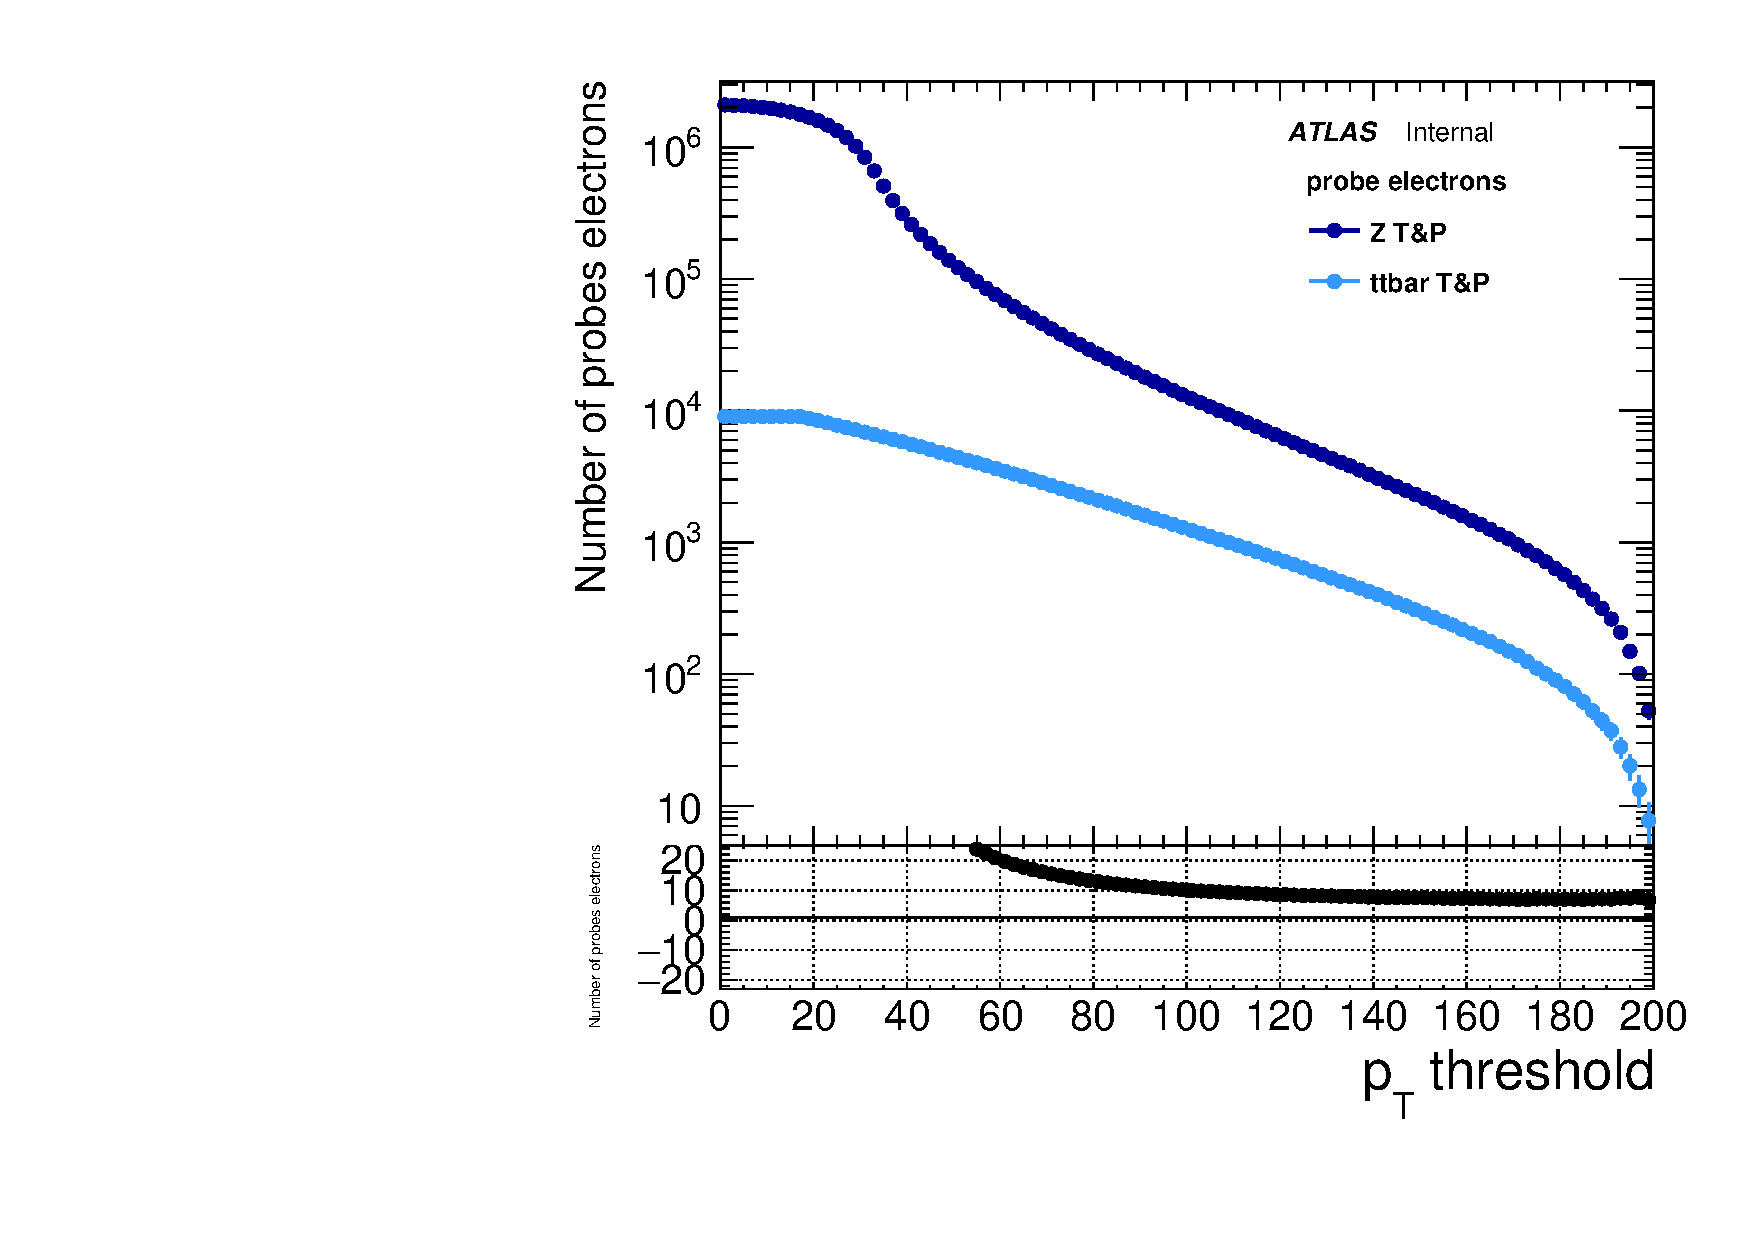
\includegraphics[width=0.4\textwidth]{BKG/realEff/Z_To_ttbar/ZTandP_Vs_ttbarTandP_baseline_electrons_Stat_Vs_PtThresh.pdf} 
	   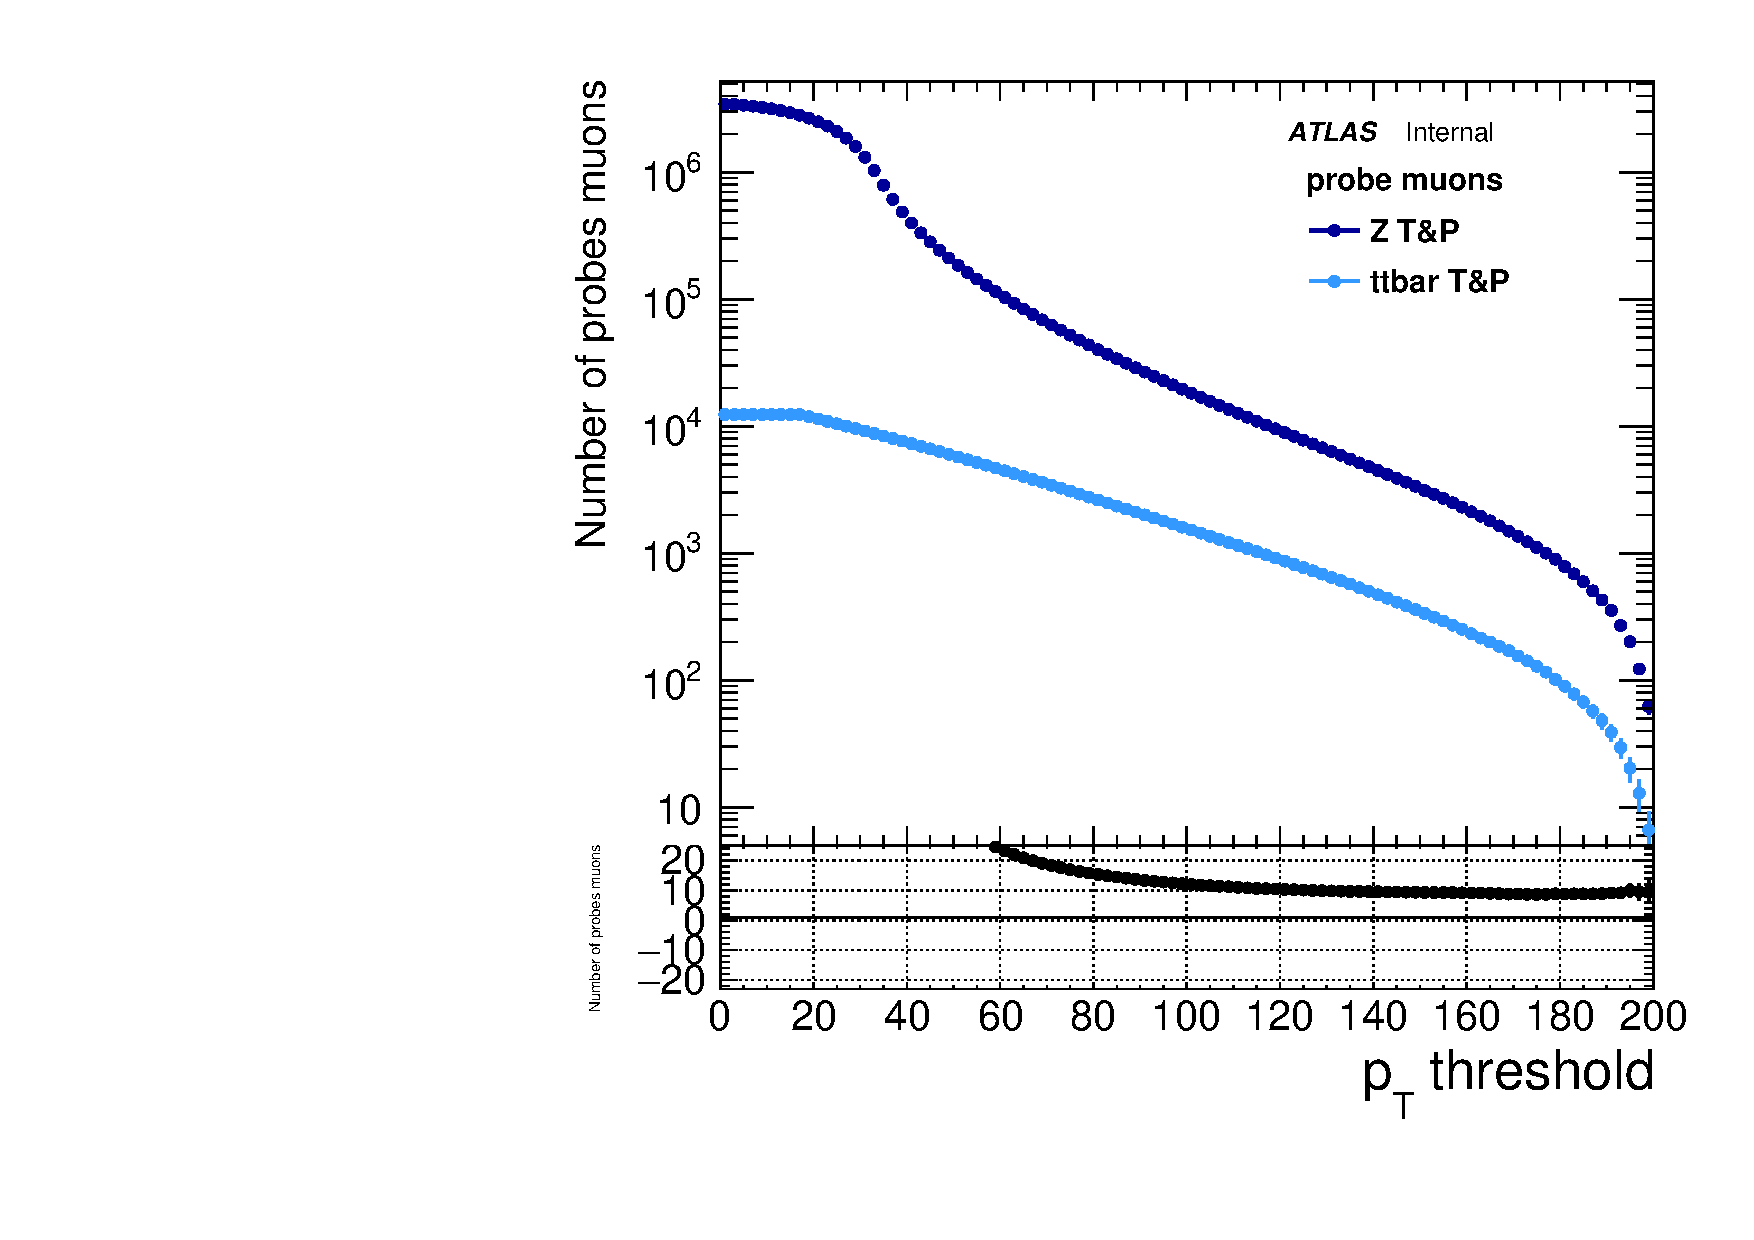
\includegraphics[width=0.4\textwidth]{BKG/realEff/Z_To_ttbar/ZTandP_Vs_ttbarTandP_baseline_muons_Stat_Vs_PtThresh.pdf}
	   \caption{\label{fig:Z_Vs_ttbar_Cumul_pt_distributions} Total number of probe leptons normalized to $3\textnormal{fb}^{-1}$ luminosity as a function of the considered $p_T$ threshold. The leptons are extracted with the $Z$ (dark blue) and $t\overline{t}$ (light blue) tag-and-probe method from their relevant Monte Carlo samples.}
	  \end{center}
	\end{figure}	
%%%%%%%%%%%%%%%%%%%%%%%%%%%%%%%%%%%%%%%%%%%%%%%%%%%%%%%%%%%%
		
		Figure \ref{fig:Z_Vs_ttbar_DRjet_distributions} shows the $\Delta R(\ell,\mathrm{jet})$ distribution extracted from $Z$ and $t\overline{t}$ events normalized to $3\textnormal{fb}^{-1}$ of luminosity. No statistical gain is seen at low $\Delta R(\ell,\mathrm{jet})$. This show that the statistical gain for the real lepton efficiency measurement induced by the $t\overline{t}$ tag-and-probe is marginal.\\ 
		
		
%%%%%%%%%%%%%%%%%%%%%%%%%%%%%%%%%%%%%%%%%%%%%%%%%%%%%%%%%%%%	
	\begin{figure}[!htb]
	  \begin{center} 
	   \includegraphics[width=0.4\textwidth]{BKG/realEff/Z_To_ttbar/ZTandP_Vs_ttbarTandP_baseline_DRjet_electrons_distributions} 
	   \includegraphics[width=0.4\textwidth]{BKG/realEff/Z_To_ttbar/ZTandP_Vs_ttbarTandP_baseline_DRjet_muons_distributions.pdf}
	   \caption{\label{fig:Z_Vs_ttbar_DRjet_distributions} $\Delta R(\ell,\mathrm{jet})$ Distribution of the probe leptons extracted with the $Z$ and the $t\overline{t}$ tag-and-probe method from relevant Monte Carlo samples normalized to $3\textnormal{fb}^{-1}$ luminosity. The left plot corresponds to the probe electrons and the the right one to the probe muons.}
	  \end{center}
	\end{figure}	
%%%%%%%%%%%%%%%%%%%%%%%%%%%%%%%%%%%%%%%%%%%%%%%%%%%%%%%%%%%%	


	\par{\bf Real efficiency comparisons\\}	
	
	The top plots from Figure \ref{fig:Z_Vs_ttbar_RealEff} show the real lepton efficiency computed with either the $Z$ or the $t\overline{t}$ tag-and-probe method. The top plots shows the real lepton efficiency as a function the lepton $p_T$. The real electron efficiency computed with the $t\overline{t}$ tag-and-probe method is $\sim 4\%$ lower that the one computed with the $Z$ tag-and-probe method for $p_T <$ 60 GeV and $\sim 2\%$ lower for $p_T >$ 60 GeV range. The real muon efficiency computed with the $t\overline{t}$ tag-and-probe method is $\sim6\%$ lower that the one computed with the $Z$ tag-and-probe method in the 30 $< p_T <$ 35 GeV range and decreases with $p_T$. Almost no efficiency differences is see for the $p_T >$ 80 GeV range.\\ 
	As the topology of the $t\overline{t}$ events is closer to the ones selected by the signal regions of the analysis than the $Z\rightarrow ll$ ones, a better estimation of the real lepton efficiency can be performed using the $t\overline{t}$ tag-and-probe method. The error bars from Figure \ref{fig:Z_Vs_ttbar_RealEff} are corresponding the estimation of the statistical errors with 3 $\mathrm{fb}^{-1}$ of data. This shows that with $~10~\mathrm{fb}^{-1}$ of statistics, the statistics will be large enough for a efficiency measurement using leptons from $t\overline{t}$. This will then reduce the SUSY signal topology extrapolation systematic described in Section \ref{App:RealEff_Z_Syst}.
	
	
%%%%%%%%%%%%%%%%%%%%%%%%%%%%%%%%%%%%%%%%%%%%%%%%%%%%%%%%%%%%	
	\begin{figure}[!htb]
	  \begin{center} 
	   \includegraphics[width=0.4\textwidth]{BKG/realEff/Z_To_ttbar/ZTandP_Vs_ttbarTandP_RealEfficiencies_Vs_pt_electrons.pdf} 
	   \includegraphics[width=0.4\textwidth]{BKG/realEff/Z_To_ttbar/ZTandP_Vs_ttbarTandP_RealEfficiencies_Vs_pt_muons.pdf}
	   \includegraphics[width=0.4\textwidth]{BKG/realEff/Z_To_ttbar/ZTandP_Vs_ttbarTandP_RealEfficiencies_Vs_eta_electrons.pdf} 
	   \includegraphics[width=0.4\textwidth]{BKG/realEff/Z_To_ttbar/ZTandP_Vs_ttbarTandP_RealEfficiencies_Vs_eta_muons.pdf}
	   \caption{\label{fig:Z_Vs_ttbar_RealEff} Real electron (left) and muon (right) efficiency efficiency computed using the $Z$ (dark blue) and the $t\overline{t}$ (light blue) tag-and-probe method using relevant Monte Carlo samples. The top (bottom) plot shows the real lepton efficiency computed as a function $p_T$ ($|\eta|$). The real efficiencies as a function of $|\eta|$ are computed considering only electron with $\pt > 30$ GeV. The statistical error bars are computed with the expected statistics at $3 fb^{-1}$. }
	  \end{center}
	\end{figure}	
%%%%%%%%%%%%%%%%%%%%%%%%%%%%%%%%%%%%%%%%%%%%%%%%%%%%%%%%%%%%	
